\part{Preliminaries}
    \chapter{Set Theory}
        This chapter will cover the necessary prerequisites before we dive into
        the various areas of mathematical analysis. This will include a short
        course on set theory and logic. We will develop set theory from the
        axioms known as Zermelo-Fraenkel Set Theory, together with the Axiom of
        Choice, commonly abbreviated as ZFC.
        \section{Basic Notions}
    \begin{ldefinition}{Sets}{Sets}
        A \gls{set} is a collection of objects, called elements, none of which
        is the set itself. Given a set $A$ and an element $x$, we denote that
        $x$ is contained in $A$ by writing $x\in{A}$. If $x$ is not an
        element of $A$, we write $x\notin{A}$.
    \end{ldefinition}
    The notion of a \textrm{set} is often left undefined, and we haven't
    defined it very well here, either. The terms \textit{collection} and
    \textit{object} have not been defined, and thus this definition is
    somewhat meaningless. Intuitively, a set is a bunch of things that we can
    discuss, either by the properties these things have, or by listing them
    out.
    \begin{lexample}{Basic Sets}{Example_of_Basic_Sets}
        When possible it is convenient to simply list out the elements of a
        set. The standard notation is to enclose the elements in braces,
        separated by commas.
        \begin{equation}
            A=\{\,1,\,2,\,3\,\}
        \end{equation}
        Here, $A$ is a set and it is entirely determined by the elements 1, 2,
        and 3. Sets need not only be concerned with numbers, and we can allow
        for abstract objects.
        \par
        \begin{subequations}
            \begin{minipage}[b]{0.49\textwidth}
                \centering
                \begin{equation}
                    B=\{\,a,\,b,\,c\,\}
                \end{equation}
            \end{minipage}
            \hfill
            \begin{minipage}[b]{0.49\textwidth}
                \centering
                \begin{equation}
                    C=\{\,\textrm{Boston, New York}\,\}
                \end{equation}
            \end{minipage}
        \end{subequations}
        \par\vspace{2.5ex}
        Both of these are valid sets.
    \end{lexample}
    \begin{lexample}{}{Sets_with_Ellipses}
        The examples described in Ex.~\ref{ex:Example_of_Basic_Sets} are all
        finite and contain a small number of elements. For larger sets we use
        ellipses to indicate some pattern. For example:
        \par
        \begin{subequations}
            \begin{minipage}[b]{0.49\textwidth}
                \centering
                \begin{align}
                    \mathbb{Z}_{3}&=\{\,1,\,2,\,3\,\}\\
                    \mathbb{Z}_{4}&=\{\,1,\,2,\,3,\,4\,\}
                \end{align}
            \end{minipage}
            \hfill
            \begin{minipage}[b]{0.49\textwidth}
                \centering
                \begin{align}
                    \mathbb{Z}_{6}  &=\{\,1,\,2,\,\dots,\,5,\,6\,\}\\
                    \mathbb{Z}_{108}&=\{\,1,\,2,\,\dots,\,107,\,108\,\}
                \end{align}
            \end{minipage}
        \end{subequations}
        \par\vspace{2.5ex}
        For infinite sets it is best to use what is known as
        \textit{Set-Builder} notation, but when a pattern is clear enough
        ellipses can suffice. The set of natural numbers and the set of
        integers are often described this way:
        \begin{subequations}
            \begin{align}
                \label{eqn:Natural_Numbers_Ellipses}%
                \mathbb{N}&=\{\,1,\,2,\,3,\,\dots\,\}\\
                \label{eqn:Integers_Ellipses}%
                \mathbb{Z}&=\{\,\dots,\,\minus{3},\,\minus{2},\,\minus{1},\,
                                0,\,1,\,2,\,3,\,\dots\,\}
            \end{align}
        \end{subequations}
        Rigorous definitions for both of these sets will be given after we've
        developed set theory more thoroughly.
    \end{lexample}
    The requirement that a set cannot contain itself is to avoid various
    paradoxes, such as the one discovered by Bertrand Russell in 1901. To
    avoid such problems, Ernst Zermello proposed a collection of
    \textit{axioms} in 1908. Subtle problems were pointed out by Abraham
    Fraenkel in 1921, and eventually the system known as Zermelo-Fraenkel
    Set Theory came to be. The condition that a set cannot contain itself can
    be restated as the \textit{Axiom of Regularity}. It is phrased as follows:
    \begin{axiom}[Axiom of Regularity]
        \label{ax:Axiom_of_Regularity}%
        If $A$ is a non-empty set, then there is a set $B\in{A}$
        such that that $A$ and $B$ are disjoint.
    \end{axiom}
    We've yet to discuss what empty and non-empty means, nor have we discussed
    the definition of disjoint. Intuitively, non-empty means the set has
    \textit{something} contained in it, and disjoint sets are sets with
    nothing in common. That is, none of their elements are the same. The axiom
    of regularity implies that, given a set $A$, it is impossible for $A$
    to be an element of $A$.
    \begin{axiom}[Axiom of the Empty Set]
        \label{ax:Axiom_of_the_Empty_Set}%
        There exists a set $\emptyset$ such that, if $x$ is an element,
        then $x\notin\emptyset$.
    \end{axiom}
    This axiom is used to define and justify the existence of the empty set.
    \begin{ldefinition}{The Empty Set}{Empty_Set}
        The \gls{empty set} is the set $\emptyset$ such that,
        for all $x$, it is true that $x\notin\emptyset$.
    \end{ldefinition}
    The empty set contains no elements and we occasionally write
    $\emptyset=\{\}$. It is unique. Note that the empty set is different from
    the set $\{\emptyset\}$. Indeed, this would violate our requirement that
    sets do not contain themselves. The empty set contains no elements,
    whereas $\{\emptyset\}$ contains one element (It contains the empty set).
    \subsection{Subsets}
        A set is determined entirely by it's elements. Thus repetition of
        elements cannot be accounted for, and the sets $\{a,\,b\}$ and
        $\{a,\,a,\,b\}$ must be considered the same, since they have exactly
        the same elements. Similarly, $\{a,\,b\}$ and $\{b,\,a\}$ are the
        same. To distinguish between such things requires a notion of order.
        This is achieved by introducing the notions of \textit{ordered pairs}
        and \textit{functions}. To rigorously show that the three
        aforementioned sets are indeed the same will require a definition of
        equality.
        \begin{ldefinition}{Subsets}{Subsets}
            A \gls{subset} of a set $B$ is a set $A$, denoted $A\subseteq{B}$,
            such that for all $x\in{A}$, it is true that $x\in{B}$. We write
            $A\nsubseteq{B}$ to denote that $A$ is not a subset of $B$.
        \end{ldefinition}
        We can often picture sets and subsets as blobs in the plane
        (Fig.~\ref{fig:Subset_Blobs}). In this figure, the blob $A$ is
        entirely contained within the blob $B$, and thus $A$ is a subset of
        $B$. The definition of subset allows us to rigorously define the
        notion of equality.
        \begin{figure}[H]
            \centering
            %--------------------------------Dependencies----------------------------------%
%   tikz                                                                       %
%-------------------------------Main Document----------------------------------%
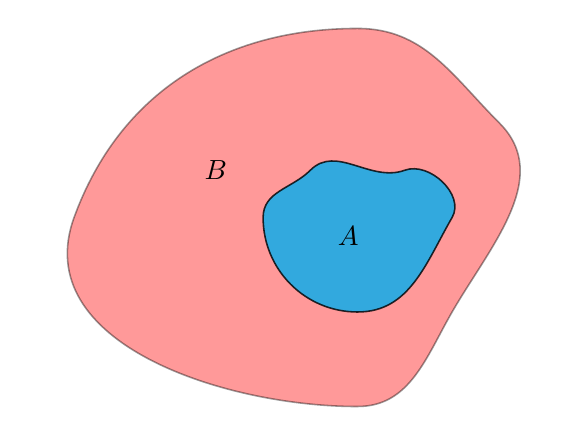
\begin{tikzpicture}[line width=0.2mm, scale=1.2]

    % Coordinates for the bigger blob.
    \coordinate (P1) at ( 0.0, -2.0);
    \coordinate (P2) at ( 1.0, -1.0);
    \coordinate (P3) at ( 1.5,  1.0);
    \coordinate (P4) at ( 0.0,  2.0);
    \coordinate (P5) at (-3.0,  0.0);

    % Coordinates for the inner blob.
    \coordinate (Q1) at ( 0.0, -1.0);
    \coordinate (Q2) at ( 1.0,  0.0);
    \coordinate (Q3) at ( 0.5,  0.5);
    \coordinate (Q4) at (-0.5,  0.5);
    \coordinate (Q5) at (-1.0,  0.0);

    % Coordindates to label things.
    \coordinate (A) at (-0.1, -0.2);
    \coordinate (B) at (-1.5,  0.5);

    % Draw the bigger blob.
    \draw[fill=red, opacity=0.4] (P1) to [out=0,    in=-120] (P2)
                                      to [out=60,   in=-45]  (P3)
                                      to [out=135,  in=0]    (P4)
                                      to [out=-180, in=70]   (P5)
                                      to [out=-110, in=-180] cycle;

    % Draw the inner blob.
    \draw[fill=cyan, opacity=0.8] (Q1) to [out=0,    in=-120]  (Q2)
                                       to [out=60,   in=20]    (Q3)
                                       to [out=-160, in=45]    (Q4)
                                       to [out=-135, in=90]    (Q5)
                                       to [out=-90,  in=180]   cycle;

    % Labels for the two blobs.
    \node at (A) {$A$};
    \node at (B) {$B$};
\end{tikzpicture}

            \caption[Visual for Subsets]
                    {Sets can be Visualized as Blobsin the Plane.}
            \label{fig:Subset_Blobs}
        \end{figure}
        \begin{lexample}{Subsets}{Basic_Subsets}
            If we let $A$ and $B$ be the sets defined by:
            \par
            \begin{subequations}
                \begin{minipage}[b]{0.49\textwidth}
                    \centering
                    \begin{equation}
                        A=\{\,1,\,2,\,3\,\}
                    \end{equation}
                \end{minipage}
                \hfill
                \begin{minipage}[b]{0.49\textwidth}
                    \centering
                    \begin{equation}
                        B=\{\,1,\,2,\,3,\,4,\,5\,\}
                    \end{equation}
                \end{minipage}
            \end{subequations}
            \par\vspace{2.5ex}
            Then we see that $A$ is a subset of $B$ since every element of
            $A$ is also an element of $B$. To express this, we write
            $A\subseteq{B}$. However, $B$ is not a subset of $A$ since the
            element 4 is contained in $B$ but it is not contained in $A$.
            Thus we may write $B\nsubseteq{A}$, indicating that $B$ is not a
            subset of $A$. Furthermore, if we define:
            \begin{equation}
                C=\{\,4,\,5,\,6,\,7,\,8\,\}
            \end{equation}
            Then we see that neither $B$ is a subset of $C$, nor is $C$ a
            subset of $B$. That is, $B\nsubseteq{C}$ and $C\nsubseteq{B}$.
            This is because $B$ has elements that aren't in $C$, and
            $C$ has elements that aren't in $B$. Moreover, $A$ and $C$ have
            zero elements in common, and are thus said to be
            \textit{disjoint}.
        \end{lexample}
        From the definition of subsets we see that for any set $A$ it is
        true that $A$ is a subset of itself. That is, $A\subseteq{A}$. It
        would be useful to distinguish between subsets that aren't the entire
        set. Such beings are called proper subsets.
        \begin{ldefinition}{Equal Sets}{Equal_Sets}
            \Glspl{equal set} are sets $A$ and $B$, denoted $A=B$, such that
            $A\subseteq{B}$ and $B\subseteq{A}$.
        \end{ldefinition}
        \begin{lexample}{Equal Sets}{Equal_Sets}
            As stated before, sets do not have a notion of order,
            nor can they account for repetition. For let $A$ and $B$
            be sets defined by:
            \par
            \begin{subequations}
                \begin{minipage}[b]{0.49\textwidth}
                    \centering
                    \begin{equation}
                        A=\{\,a,\,b\,\}
                    \end{equation}
                \end{minipage}
                \hfill
                \begin{minipage}[b]{0.49\textwidth}
                    \centering
                    \begin{equation}
                        B=\{\,a,\,a,\,b\,\}
                    \end{equation}
                \end{minipage}
            \end{subequations}
            \par\vspace{2.5ex}
            Then $A=B$. For $A\subseteq{B}$, since for all $x\in{A}$, it is
            true that $x\in{B}$. But also $B\subseteq{A}$, since if
            $x\in{B}$ then either $x=a$ or $x=b$. But $a$ and $b$ are elements
            of $A$ and thus, if $x\in{B}$, then it is true that $x\in{A}$
            and therefore $B\subseteq{A}$. By the definition of equality
            (Def.~\ref{def:Equal_Sets}), $A=B$. If we further define:
            \begin{equation}
                C=\{b,\,a\}
            \end{equation}
            Then again we see that $A=C$, since $A\subseteq{C}$ and
            $C\subseteq{A}$.
        \end{lexample}
        Zermelo-Fraenkel set theory defines equality via
        the \textit{Axiom of Extensionality}:
        \begin{axiom}[Axiom of Extensionality]
            If $A$ and $B$ are sets, and if for all $x$ it is true that
            $x\in{A}$ if and only if $x\in{B}$, then $A=B$.
        \end{axiom}
        This is precisely what we've stated, but we've used the language of
        subsets. Also, rather than stating equality as an axiom, we've
        presented it as a definition. The differences are purely semantical.
        We can now define proper subsets.
        \begin{ldefinition}{Proper Subset}{Proper_Subset}
            A \gls{proper subset} of a set $B$ is a set $A\subseteq{B}$,
            denoted $A\subsetneq{B}$, such that $A\ne{B}$.
        \end{ldefinition}
        The symbols $\subseteq$ and $\subsetneq$ are analogous to the
        notations of inequalities that one finds in calculus: $\leq$ and $<$.
        In many texts, the two symbols $\subseteq$ and $\subset$ are taken to
        be identical, which may cause confusion. In an attempt to reduce
        confusion, $\subseteq$ will denote any subset, $\subsetneq$ denotes a
        proper subset, and the symbol $\subset$ will be avoided.
        \begin{lexample}{Proper Subsets}{Proper_Subsets}
            Let $A$ and $B$ be sets defined as follows:
            \par
            \begin{subequations}
                \begin{minipage}[b]{0.49\textwidth}
                    \centering
                    \begin{equation}
                        A=\{\,a,\,b,\,c\,\}
                    \end{equation}
                \end{minipage}
                \hfill
                \begin{minipage}[b]{0.49\textwidth}
                    \centering
                    \begin{equation}
                        B=\{\,a,\,b,\,c,\,d\,\}
                    \end{equation}
                \end{minipage}
            \end{subequations}
            \par\vspace{2.5ex}
            Then $A\subseteq{B}$, since every element of $A$ is an element of
            $B$, but $B\nsubseteq{A}$ since $d\in{B}$ and $d\notin{A}$.
            Therefore $A\ne{B}$, and thus $A$ is a  proper subset of $B$.
            We denote this by writing $A\subsetneq{B}$.
        \end{lexample}
    \subsection{Ordered Pairs and Cartesian Products}
        Before we can begin stating and proving theorems, we need an
        indispensable tool: \textit{The Law of the Excluded Middle}. This
        states that, given a proposition $P$, either $P$ is true or $P$ is
        not true. It allows us to prove theorems via
        \textit{proof by contradiction}. That is, we assume the opposite and
        arrive at a contradiction, thus proving the original statement was
        true. The law of the excluded middle is a theorem, known as
        Diaconescu's Theorem, that follows from the \textit{Axiom of Choice}.
        This is a very strong, but controversial, axiom of set theory. It is
        common in analysis to adopt the axiom, and it's use is widespread in
        many theorems. To discuss the axiom of choice we first need to
        develop the notions of function and union.
        \begin{axiom}[Axiom of Pairing]
            \label{ax:Axiom_of_Pairing}%
            If $a$ and $b$ are elements, then there is a set $A$ such that
            $z\in{A}$ if and only if either $z=a$ or $z=b$. That is,
            $A=\{\,a,\,b\,\}$.
        \end{axiom}
        The axiom of pairing simply states that, given two things, we can
        form a set that is defined entirely by these two things. This is
        used to proved \textit{ordered pairs} exist.
        \begin{theorem}
            \label{thm:Existence_of_Ordered_Pair}%
            If $x$ and $y$ are elements, then there exists a set $A$ such
            that $z\in{A}$ if and only if $z=\{\,x\,\}$ or $z=\{\,x,\,y\,\}$.
        \end{theorem}
        \begin{proof}
            For let $a=x$ and $b=x$. Then, by the axiom of pairing
            (Ax.~\ref{ax:Axiom_of_Pairing}), there is a set
            $\{\,a,\,b\,\}=\{\,x,\,x\,\}$. But by the definition of equality
            (Def.~\ref{def:Equal_Sets}), $\{\,x,\,x\,\}=\{\,x\,\}$. Again, by
            the axiom of pairing, letting $a=x$ and $b=y$, we have that the
            set $\{\,x,\,y\,\}$ exists. Finally, invoking the axiom of
            pairing, and letting $a=\{\,x\,\}$ and $b=\{\,x,\,y\,\}$, we have
            that the set $\{\,\{\,x\,\},\,\{\,x,\,y\,\}\,\}$ exists.
        \end{proof}
        \begin{ldefinition}{Ordered Pair}{Ordered_Pair}
            The \gls{ordered pair} of an element $x$ with respect
            to an element $y$ is the set:
            \begin{equation}
                (x,\,y)\equiv\big\{\,\{\,x\,\},\,\{\,x,\,y\,\}\,\big\}
            \end{equation}
            Where the symbol $\equiv$ used here means ``Is defined by.''
        \end{ldefinition}
        Thm.~\ref{thm:Existence_of_Ordered_Pair} allows us to define ordered
        pairs in a manner that is consistent with ZFC. That is, if the axioms
        we are adopting are consistent, then so is our definition. Note that
        from the definition, given two distinct elements $x$ and $y$,
        $(x,\,y)\ne(y,\,x)$. This definition is due to Kazimierz Kuratowski
        and was first put forward in 1921. It does precisely what we want for
        an ordered pair, and distinguishes the order of the elements. There
        is a slight caveat, for we have the following reduction:
        \begin{equation}
            (x,\,x)=\big\{\,\{\,x\,\},\,\{\,x,\,x\,\}\,\big\}
                   =\big\{\,\{\,x\,\},\,\{\,x\,\}\,\big\}
                   =\big\{\,\{\,x\,\}\,\big\}
        \end{equation}
        This does not create too much of an issue.
        An alternative definition was put forward by Norbert Wiener in 1914:
        \begin{equation}
            (x,\,y)_{W}=\Big\{\,\big\{\{x\},\,\emptyset\big\},\,
                                \big\{\{y\}\big\}\Big\}
        \end{equation}
        Wiener used this definition since he was interested in things called
        \textit{types}. This is connected to Bertrand Russell's Type Theory,
        which was an attempt to free set theory of the paradoxes he
        discovered. Kuratowski's definition is sufficient for almost all
        purposes, and it's the one we shall adopt.
        \begin{lexample}{}{Ordered_Pair_1_2_vs_2_1}
            Consider the ordered pair $(1,\,2)$, where we take for granted
            that $1\ne{2}$. Using Kuratowski's definition
            (Def.~\ref{def:Ordered_Pair}), we obtain:
            \begin{equation}
                (1,\,2)=\big\{\,\{\,1\,\},\,\{\,1,\,2\,\}\,\big\}
            \end{equation}
            Swapping and computing $(2,\,1)$, we have:
            \begin{equation}
                (2,\,1)=\big\{\,\{\,2\,\},\,\{\,2,\,1\,\}\,\big\}
            \end{equation}
            Now the sets $\{1,\,2\}$ and $\{2,\,1\}$ are equal, since they
            contain the same elements. Therefore $\{1,\,2\}$ is an element
            of both $(1,\,2)$ and $(2,\,1)$. However $\{1\}$ is an element
            of $(1,\,2)$, and not and element of $(2,\,1)$, and thus
            $(1,\,2)\nsubseteq(2,\,1)$. Similarly, $\{2\}$ is an element of
            $(2,\,1)$, but not an element of $(1,\,2)$, and thus
            $(2,\,1)\nsubseteq(1,\,2)$. Thus, we have that
            $(1,\,2)\ne(2,\,1)$, as desired.
        \end{lexample}
        To order sets that have more than two
        elements we must first define functions. Functions are defined in
        terms of the \textit{Cartesian Product} of two sets. To do this we
        need another axiom from Zermelo-Fraenkel Set Theory: The
        \textit{Axiom Schema of Specification}. This allows us to construct
        sets via \textit{Set-Builder Notation}.
        \begin{axiom}[Axiom Schema of Specification]
            \label{ax:Axiom_Schema_of_Specification}%
            If $B$ is a set and $P$ is a proposition, then there is a set
            $A\subseteq{B}$ such that $x\in{A}$ if and only if $x\in{B}$ and
            $P(x)$ is true.
        \end{axiom}
        This axiom states that the Set-Builder method of constructing sets is
        valid. We have seen that the natural numbers $\mathbb{N}$ and the
        integers $\mathbb{Z}$ (From the German \textit{Zahl}) can be loosely
        described by using ellipses to indicate a pattern
        (Eqns.~\ref{eqn:Natural_Numbers_Ellipses}-%
        \ref{eqn:Integers_Ellipses}, respectively). It would be more
        difficult (But not impossible) to describe the set of rational
        numbers in such a way. Instead, we use set
        builder notation. We can describe the set of rational numbers
        $\mathbb{Q}$ as follows:
        \begin{equation}
            \mathbb{Q}=\Big\{\;\frac{p}{q}\in\mathbb{R}\,:
                               \,p,\,q\in\mathbb{Z}
                               \textrm{ and }q\ne{0}\;\Big\}
        \end{equation}
        That is, the rational numbers are the set of all real numbers which
        can be written as the ratios of integers with non-zero denominator.
        The Axiom Schema of Specification states that this is is a valid
        method of describing sets. It is also known as the axiom of
        separation.
        \par\hfill\par
        It is crucial to note the requirement that the set we our building
        with our proposition is a subset of some larger set. For
        $\mathbb{Q}$ we assumed there exists some set $\mathbb{R}$ (The
        real numbers). The axiom does not allow us to simply write
        \textit{The set of all $x$ such that $P(x)$ is true}. Indeed, this is
        precisely how one arrives at Russell's paradox. The axiom
        allows us to write
        \textit{The set of all $x$ such that $x\in{B}$ and $P(x)$ is true},
        where $B$ is some set whose existence has already been established.
        \begin{lexample}{Set-Builder Notation}{Set_Builder_Evens_and_Odds}
            Again supposing that the natural numbers have been defined for us,
            we can use this to construct other sets. An even natural number
            is an integer $n\in\mathbb{N}$ such that $n/2$ is also an integer.
            Similarly, an odd natural number is a an integer $n\in\mathbb{N}$
            such that $n$ is not even. We can describe the sets of even and
            odd numbers via ellipses, and we write:
            \par
            \begin{subequations}
                \begin{minipage}[b]{0.49\textwidth}
                    \centering
                    \begin{equation}
                        \mathbb{N}_{e}=\{\,2,\,4,\,6,\,8,\,\dots\,\}
                    \end{equation}
                \end{minipage}
                \hfill
                \begin{minipage}[b]{0.49\textwidth}
                    \centering
                    \begin{equation}
                        \mathbb{N}_{o}=\{\,1,\,3,\,5,\,7,\,\dots\,\}
                    \end{equation}
                \end{minipage}
            \end{subequations}
            \par\vspace{2.5ex}
            But rather than doing this, we can introduce rigor and describe
            these sets using Set-Builder notation. We write:
            \par
            \begin{subequations}
                \begin{minipage}[b]{0.49\textwidth}
                    \centering
                    \begin{equation}
                        \mathbb{N}_{e}=\{\;n\in\mathbb{N}:
                                           n\textrm{ is even.}\;\}
                    \end{equation}
                \end{minipage}
                \hfill
                \begin{minipage}[b]{0.49\textwidth}
                    \centering
                    \begin{equation}
                        \mathbb{N}_{o}=\{\;n\in\mathbb{N}:
                                           n\textrm{ is odd.}\;\}
                    \end{equation}
                \end{minipage}
            \end{subequations}
            \par\vspace{2.5ex}
            Such notation is justified by the axiom schema of specification.
        \end{lexample}
        Next, we discuss the \textit{axiom of union}.
        \begin{axiom}[Axiom of Union]
            \label{ax:Axiom_of_Union}%
            If $\mathcal{O}$ is a set, then there is a set $A$ such that, for
            all $x$, $x\in{A}$ if and only if there is an $F\in\mathcal{O}$
            such that $x\in{F}$.
        \end{axiom}
        This states that given a collection of sets, we can form a new sets
        whose elements are the elements of the sets in our collection. This
        is best illustrated by example.
        \begin{lexample}{Axiom of Union}{Axiom_of_Union}
            Let $A$ and $B$ be sets defined as follows:
            \par
            \begin{subequations}
                \begin{minipage}[b]{0.49\textwidth}
                    \centering
                    \begin{equation}
                        A=\{\,1,\,2,\,3\,\}
                    \end{equation}
                \end{minipage}
                \hfill
                \begin{minipage}[b]{0.49\textwidth}
                    \centering
                    \begin{equation}
                        B=\{\,2,\,3,\,4\,\}
                    \end{equation}
                \end{minipage}
            \end{subequations}
            \par
            \vspace{2.5ex}
            Using the axiom of pairing, we can create the following set:
            \begin{equation}
                \mathcal{O}=\{\,A,\,B\,\}
            \end{equation}
            The axiom of union says that we can form a new set $C$ defined as
            the set of all elements contained in either $A$ or $B$:
            \begin{equation}
                C=\{\,1,\,2,\,3,\,4\,\}
            \end{equation}
            This construction, which combines the axiom of pairing and the
            axiom of union, can be used to define the union of two sets. And
            indeed, the axiom of union can be used to define union of
            arbitrarily many sets.
        \end{lexample}
        \begin{theorem}
            \label{thm:Union_of_Sets_Exists}%
            If $A$ and $B$ are sets, then there is a set $C$ such that, for
            all $x$, $x\in{C}$ if and only if $x\in{A}$ or $x\in{B}$, or both.
        \end{theorem}
        \begin{proof}
            For by the axiom of pairing (Ax.~\ref{ax:Axiom_of_Pairing}), if
            $A$ and $B$ are sets then there is a set $\mathcal{O}$ such
            that $\mathcal{O}=\{\,A,\,B\,\}$. But then by the axiom of union
            (Ax.~\ref{ax:Axiom_of_Union}) there is a set $C$ such that, for
            all $x$, $x\in{C}$ if and only if there is a set $F\in\mathcal{O}$
            such that $x\in{F}$. But then $x\in{C}$ if and only if either
            $x\in{A}$ or $x\in{B}$, or both.
        \end{proof}
        \begin{fdefinition}{Union of Two Sets}{Union_of_Two}
            The \gls{union of two sets}, $A$ and $B$, is the set
            $A\cup{B}$ define by:
            \begin{equation}
                A\cup{B}=\{\;x\,:\,x\in{A}\textrm{ or }x\in{B}\;\}
            \end{equation}
        \end{fdefinition}
        Thm.~\ref{thm:Union_of_Sets_Exists} justifies
        Def.~\ref{def:Union_of_Two}. Unions can be visualized by the use of
        Venn Diagrams (Fig.~\ref{fig:Venn_Diagram_Union}). The union of two
        sets is a commonly used construction in all branches of mathematics.
        Various theorems about it will be proved when we delve more into the
        various set operations, but we still need the law of the excluded
        middle to prove these. The last stepping stone is the axiom of the
        power set, which allows us to justify these various constructions.
        \begin{figure}[H]
            \centering
            %--------------------------------Dependencies----------------------------------%
%   tikz                                                                       %
%-------------------------------Main Document----------------------------------%
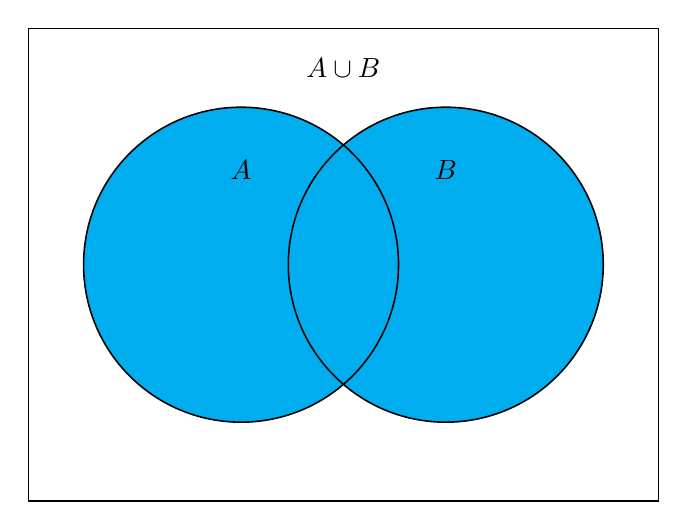
\begin{tikzpicture}[line width=0.2mm]

    % Coordinates for the centers of the circles.
    \coordinate (C1) at (-1.3, 0);
    \coordinate (C2) at ( 1.3, 0);

    % Coordinates for the labels.
    \coordinate (A) at (-1.3, 1.2);
    \coordinate (B) at ( 1.3, 1.2);
    \coordinate (U) at ( 0.0, 2.5);

    % Rectangle indicating the universe set.
    \draw (-4, -3) rectangle (4, 3);

    % Fill in the circle with cyan.
    \draw[fill=cyan, draw=none] (C1) circle (2);
    \draw[fill=cyan, draw=none] (C2) circle (2);

    % Give outlines to the circles.
    \draw (C1) circle (2);
    \draw (C2) circle (2);

    % Labels.
    \node at (A) {$A$};
    \node at (B) {$B$};
    \node at (U) {$A\cup{B}$};
\end{tikzpicture}
            \caption{Venn Diagram for Unions}
            \label{fig:Venn_Diagram_Union}
        \end{figure}
        \begin{lexample}{Union of Two Sets}{Union_of_Two_Sets}
            If we let $A$ and $B$ be defined as follows:
            \par
            \begin{subequations}
                \begin{minipage}[b]{0.49\textwidth}
                    \centering
                    \begin{equation}
                        A=\{\,3,\,5,\,6\,\}
                    \end{equation}
                \end{minipage}
                \hfill
                \begin{minipage}[b]{0.49\textwidth}
                    \centering
                    \begin{equation}
                        B=\{\,2,\,9,\,11,\,5\,\}
                    \end{equation}
                \end{minipage}
            \end{subequations}
            \par\vspace{2.5ex}
            We can form the union $A\cup{B}$ as follows:
            \begin{equation}
                A\cup{B}=\{\,2,\,3,\,5,\,6,\,9,\,11\,\}
            \end{equation}
            That is, the set of all elements in either $A$ or $B$, or both.
            We can do this construction with infinite sets as well:
            \par
            \begin{subequations}
                \begin{minipage}[b]{0.30\textwidth}
                    \centering
                    \begin{equation}
                        \mathbb{N}\cup\mathbb{Z}=\mathbb{Z}
                    \end{equation}
                \end{minipage}
                \hspace{0.03\textwidth}
                \begin{minipage}[b]{0.30\textwidth}
                    \centering
                    \begin{equation}
                        \mathbb{N}_{e}\cup\mathbb{N}_{o}=\mathbb{N}
                    \end{equation}
                \end{minipage}
                \hspace{0.03\textwidth}
                \begin{minipage}[b]{0.30\textwidth}
                    \centering
                    \begin{equation}
                        \mathbb{Q}\cup\mathbb{Z}=\mathbb{Q}
                    \end{equation}
                \end{minipage}
            \end{subequations}
            \par\vspace{2.5ex}
            Where $\mathbb{N}_{e}$, $\mathbb{N}_{o}$, $\mathbb{N}$,
            $\mathbb{Z}$, and $\mathbb{Q}$ denote the sets of even numbers,
            odd numbers, natural numbers, integers, and rational numbers,
            respectively,
        \end{lexample}
        \begin{axiom}[Axiom of the Power Set]
            \label{ax:Axiom_of_the_Power_Set}%
            If $A$ is a set, then there is a set $\mathcal{P}(A)$, called the
            power set, such that $x\in\mathcal{P}(A)$ if and only if
            $x\subseteq{A}$.
        \end{axiom}
        This axiom allows us to define the power set of any set.
        \begin{ldefinition}{Power Set}{Power_Set}
            The power set of a set $A$ is the set
            $\mathcal{P}(A)$ defined by:
            \begin{equation}
                \mathcal{P}(A)=\{\,B\,:\,B\subseteq{A}\,\}
            \end{equation}
            That is, $\mathcal{P}(A)$ is the set of all subsets of $A$.
        \end{ldefinition}
        \begin{theorem}
            \label{thm:Cartesian_Product_Exists}%
            If $A$ and $B$ are sets, then there is a set $C$ such that, for
            all $z$, $z\in{C}$ if and only if there exists $x\in{A}$ and
            $y\in{B}$ such that $z=(x,\,y)$.
        \end{theorem}
        \begin{proof}
            For let $\mathcal{O}=A\cup{B}$. Then by the axiom of the power set
            (Ax.~\ref{ax:Axiom_of_the_Power_Set}), the power set
            $\mathcal{P}(\mathcal{O})$ exists. But, again by the axiom of the
            power set, the power set
            $\mathcal{P}\big(\mathcal{P}(\mathcal{O})\big)$ exists. But then
            $z\in\mathcal{P}\big(\mathcal{P}(\mathcal{O})\big)$
            if and only if $z\subseteq\mathcal{P}(\mathcal{O})$, and for all
            $x\in{A}$ and $y\in{B}$,
            $(x,\,y)\subseteq\mathcal{P}(\mathcal{O})$. Let $P$ be the
            proposition $P(z)$ is true if and only if there exists $x\in{A}$
            and $y\in{B}$ such that $z=(x,\,y)$. Then, by the axiom schema of
            specification (Ax.~\ref{ax:Axiom_Schema_of_Specification}),
            there is a set $C$ such that:
            \begin{equation}
                C=\{\,z\,:\,P(z)\,\}
            \end{equation}
            Therefore, etc.
        \end{proof}
        The set $C$ constructed in Thm.~\ref{thm:Cartesian_Product_Exists} is
        the set of all ordered pairs of elements whose first entry is from the
        set $A$ and whose second entry comes from the set $B$. This is
        precisely the what we want the Cartesian product of $A$ with $B$ to
        be. Thus, this theorem gives justification to the following
        definition:
        \begin{ldefinition}{Cartesian Product}{Cartesian_Product}
            The \gls{Cartesian product} of a set $A$ with respect to a set
            $B$ is the set:
            \begin{equation}
                A\times{B}\equiv\{\;(a,\,b)\,:\,a\in{A}
                                    \textrm{ and }b\in{B}\;\}
            \end{equation}
            Where $(a,\,b)$ denotes the ordered pair of $a$ with $b$.
        \end{ldefinition}
        Much the way ordered pairs place order onto two arbitrary elements,
        Cartesian products place order on sets. Given two distinct sets $A$
        and $B$, we have that $A\times{B}\ne{B}\times{A}$, and thus the
        order in which we performed the Cartesian product is important. The
        validity of this statement stems from the fact that, in general,
        $(a,\,b)\ne(b,\,a)$, and thus if $A$ and $B$ are distinct sets they'll
        have at least some different elements, meaning $A\times{B}$ will have
        different ordered pairs than $B\times{A}$.
        \begin{lexample}{Cartesian Products}{Basic_Cartesian_Products}
            Let $A$ and $B$ be sets defined as follows:
            \par
            \begin{subequations}
                \begin{minipage}[b]{0.49\textwidth}
                    \centering
                    \begin{equation}
                        A=\{\,1,\,2,\,3\,\}
                    \end{equation}
                \end{minipage}
                \hfill
                \begin{minipage}[b]{0.49\textwidth}
                    \centering
                    \begin{equation}
                        B=\{\,a,\,b\,\}
                    \end{equation}
                \end{minipage}
            \end{subequations}
            \par\vspace{2.5ex}
            Let's compute $A\times{B}$ and $B\times{A}$. From the definition
            (Def.~\ref{def:Cartesian_Product}) we have:
            \begin{equation}
                A\times{B}=\{\;(a,b)\,:\,a\in{A}\textrm{ and }b\in{B}\;\}
            \end{equation}
            Using this, we can compute:
            \begin{equation}
                A\times{B}=\big\{\,(1,a),\,(2,a),\,(3,a),\,
                                   (1,b),\,(2,b),\,(3,b)\,\big\}
            \end{equation}
            Computing $B\times{A}$, we have:
            \begin{equation}
                B\times{A}=\big\{\,(a,\,1),\,(a,\,2),\,(a,\,3),\,
                                   (b,\,1),\,(b,\,2),\,(b,\,3)\,\big\}
            \end{equation}
            Now if we suppose that $a$ is not equal to 1, then we see that
            $(a,1)$ is a different element than $(1,a)$, and thus $A\times{B}$
            is not equal to $B\times{A}$. Next, compute $A\times{A}$:
            \begin{equation}
                A\times{A}=\big\{\,(1,1),\,(1,2),\,(1,3),\,
                                   (2,1),\,(2,2),\,(2,3),\,
                                   (3,1),\,(3,2),\,(3,3)\,\big\}
            \end{equation}
            And finally $B\times{B}$:
            \begin{equation}
                B\times{B}=\big\{\,(a,\,a),\,(a,\,b),
                                 \,(b,\,a),\,(b,\,b)\,\big\}
            \end{equation}
            Equality of $A\times{B}$ and $B\times{A}$ is achieved if and only
            if $A=B$, or if either set is the empty set.
        \end{lexample}
        Note that in Ex.~\ref{ex:Basic_Cartesian_Products}, the \textit{size}
        of the Cartesian product of two sets was simply the product of the
        number of elements of the constituent sets. That is, we see that $A$
        has three elements and $B$ has two elements, but also that
        $A\times{B}$ has six elements. Moreover, $A\times{A}$ has nine
        elements and $B\times{B}$ has four. This pattern holds for the
        Cartesian products of any two \textit{finite} sets.
        \par\hfill\par
        It is common to consider the Cartesian product of a set with itself.
        That is, given a set $A$, we are often interested in $A\times{A}$. We
        denote this by writing $A^{2}$. One such example is when we consider
        the set of real numbers, $\mathbb{R}$. The Cartesian product
        $\mathbb{R}^{2}$ is called the \textit{Euclidean Plane},
        or the \textit{Cartesian Plane}, after Euclid of Alexandria and
        Ren\'{e} Descartes. This is because $\mathbb{R}^{2}$ is used to model
        both planar geometry and analytical geometry, of which Euclid and
        Descartes were pioneers of, respectively. The term Cartesian products
        is in honor of Ren\'{e} Descartes, as well.
        \begin{lexample}{Plane Lattice}{Lattice_N_times_N}
            Consider $\mathbb{N}^{2}$, where $\mathbb{N}$ denotes the set of
            natural numbers (Eqn.~\ref{eqn:Natural_Numbers_Ellipses}), and
            $\mathbb{N}^{2}$ denotes the Cartesian product of this set with
            itself. We can visualize this by drawing a lattice of points in the
            plane (Fig.~\subref{fig:Lattice_Cart_Prod_of_N_with_N}).
        \end{lexample}
        \begin{lexample}{Cartesian Plane}{The_Plane_R_times_R}
            Let $\mathbb{R}$ denote the set of real numbers, and let
            $A=\mathbb{R}$ and $B=\mathbb{R}$. Then we have:
            \begin{equation}
                A\times{B}=\mathbb{R}\times\mathbb{R}\equiv\mathbb{R}^{2}
            \end{equation}
            Where the symbol $\equiv$ again means that $\mathbb{R}^{2}$ is
            defined by this expression. Using the definition of Cartesian
            products (Def.~\ref{def:Cartesian_Product}), we obtain:
            \begin{equation}
                \mathbb{R}^{2}=\{\;(x,y)\,:\,x\in\mathbb{R}
                                   \textrm{ and }y\in\mathbb{R}\;\}
            \end{equation}
            That is, $\mathbb{R}^{2}$ is the set of all ordered pairs of real
            numbers. The first term is called the $x$ coordinate, and
            similarly the second term is called the $y$ coordinate. This is
            used to model planar geometry (Fig.\subref{fig:Cartesian_Plane}).
        \end{lexample}
        \begin{figure}[H]
            \centering
            \begin{subfigure}[b]{0.49\textwidth}
                \centering
                \resizebox{\textwidth}{!}{
                    %--------------------------------Dependencies----------------------------------%
%   amssymb                                                                    %
%   tikz                                                                       %
%       arrows.meta                                                            %
%-------------------------------Main Document----------------------------------%
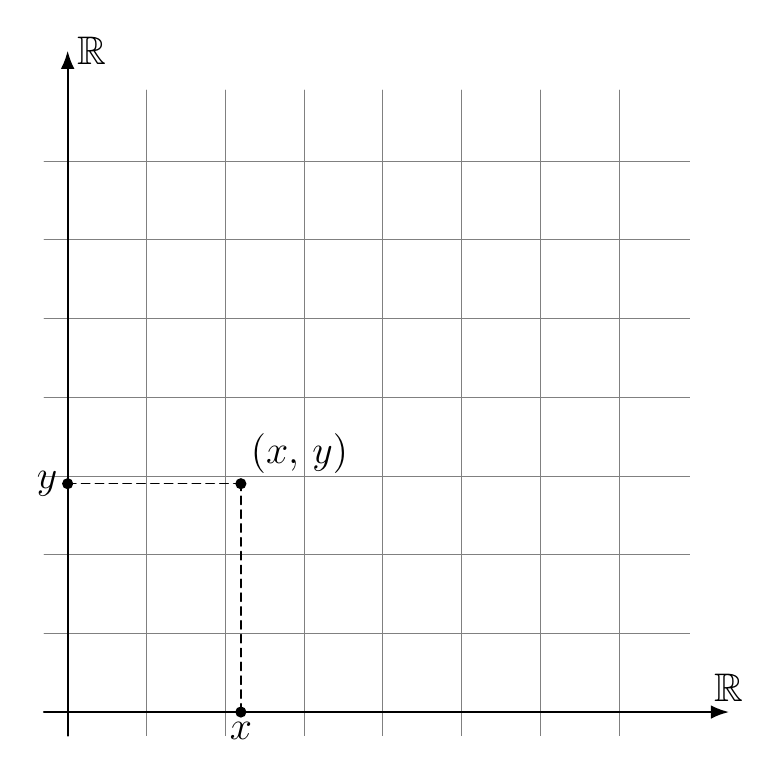
\begin{tikzpicture}[%
    >=Latex,
    line width=0.2mm,
    line cap=round,
    font=\Large
]
    % Coordinates for the points.
    \coordinate (x) at (2.2, 0.0);
    \coordinate (y) at (0.0, 2.9);
    \coordinate (z) at (2.2, 2.9);

    % Draw a grid.
    \draw[style=help lines] (-0.3, -0.3) grid (7.9, 7.9);

    % Axes.
    \begin{scope}[thick]
        \draw[->] (-0.3, 0) to (8.4, 0) node [above] {$\mathbb{R}$};
        \draw[->] (0, -0.3) to (0, 8.4) node [right] {$\mathbb{R}$};
    \end{scope}

    % Draw dashed lines to the point.
    \begin{scope}[densely dashed]
        \draw (x) to (z);
        \draw (y) to (z);
    \end{scope}

    % Draw dots marking the various points.
    \draw[fill=black] (x) circle (0.6mm);
    \draw[fill=black] (y) circle (0.6mm);
    \draw[fill=black] (z) circle (0.6mm);

    \node at (x) [below=0.1]     {$x$};
    \node at (y) [left=0.1]      {$y$};
    \node at (z) [above right]   {$(x,\,y)$};
\end{tikzpicture}%
                }
                \subcaption{The Cartesian Plane $\mathbb{R}^{2}$}
                \label{fig:Cartesian_Plane}
            \end{subfigure}
            \begin{subfigure}[b]{0.49\textwidth}
                \centering
                \resizebox{\textwidth}{!}{%
                    %--------------------------------Dependencies----------------------------------%
%   amssymb                                                                    %
%   tikz                                                                       %
%       arrows.meta                                                            %
%-------------------------------Main Document----------------------------------%
\begin{tikzpicture}[%
    >=Latex,
    line width=0.2mm,
    line cap=round
]

    % Axes.
    \begin{scope}[thick, font=\Large]
        \draw[->] (0, 0) to (8.4, 0) node [above] {$\mathbb{N}$};
        \draw[->] (0, 0) to (0, 8.4) node [right] {$\mathbb{N}$};
    \end{scope}

    \foreach\x in{1, 2, 3, 4, 5, 6, 7, 8}{
        \foreach\y in{1, 2, 3, 4, 5, 6, 7, 8}{
            \draw[fill=black] (\x, \y) circle (0.2mm);
        }
        \draw (\x, -0.1) to (\x, 0.1) node [below=1ex] {$\x$};
        \draw (-0.1, \x) to (0.1, \x) node [left=1ex]  {$\x$};
    }
\end{tikzpicture}%
                }
                \caption{The Lattice $\mathbb{N}^{2}$}
                \label{fig:Lattice_Cart_Prod_of_N_with_N}
            \end{subfigure}
            \caption{Examples of Cartesian Products}
            \label{fig:Cartesian_Products_Examples}
        \end{figure}
        \begin{lexample}{}{Generic_Cartesian_Product}
            Consider the following sets:
            \par
            \begin{subequations}
                \begin{minipage}[b]{0.49\textwidth}
                    \centering
                    \begin{equation}
                        A=\{\,\textrm{Point, Line 1, Line 2}\,\}
                    \end{equation}
                \end{minipage}
                \hfill
                \begin{minipage}[b]{0.49\textwidth}
                    \centering
                    \begin{equation}
                        B=\{\,\textrm{Point, Line}\,\}
                    \end{equation}
                \end{minipage}
            \end{subequations}
            \par\vspace{2.5ex}
            We can visually represent the Cartesian product $A\times{B}$ by
            drawing $A$ in green and $B$ in red, as shown in
            Fig.~\ref{fig:Cartesian_Product_Example}. The Cartesian Product
            $A\times{B}$ is the set formed by connecting all of the points
            from $A$ and $B$ in the plane. This is shown in blue.
        \end{lexample}
        \begin{figure}[H]
            \centering
            %--------------------------------Dependencies----------------------------------%
%   tikz                                                                       %
%       arrows.meta                                                            %
%-------------------------------Main Document----------------------------------%
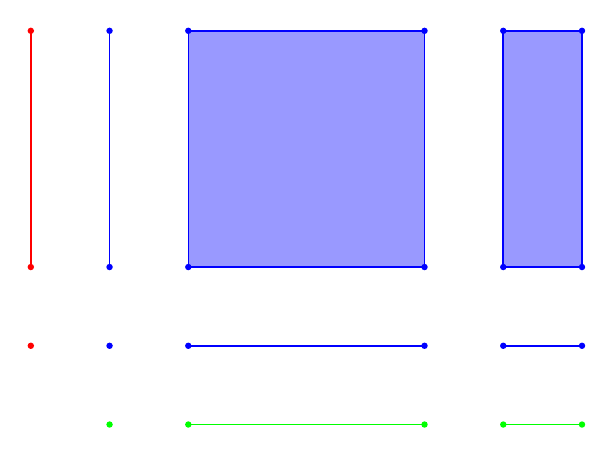
\begin{tikzpicture}[%
    >=Latex,
    line width=0.2mm,
    line cap=round
]

    % Draw green to indicate the set A.
    \begin{scope}[green]

        % Draw some points.
        \draw[fill=green] (1, 0) circle (0.3mm);
        \draw[fill=green] (2, 0) circle (0.3mm);
        \draw[fill=green] (5, 0) circle (0.3mm);
        \draw[fill=green] (6, 0) circle (0.3mm);
        \draw[fill=green] (7, 0) circle (0.3mm);

        % Draw lines.
        \draw (2, 0) to (5, 0);
        \draw (6, 0) to (7, 0);
    \end{scope}

    % Draw red to denote the set B.
    \begin{scope}[red]

        % Draw in some points.
        \draw[fill=red] (0, 1) circle (0.3mm);
        \draw[fill=red] (0, 2) circle (0.3mm);
        \draw[fill=red] (0, 5) circle (0.3mm);

        % Draw a line.
        \draw (0, 2) to (0, 5);
    \end{scope}

    % Use blue to mark AxB (Cartesian product).
    \begin{scope}[blue]

        % Fill in points.
        \draw[fill=blue] (1, 1) circle (0.3mm);
        \draw[fill=blue] (1, 2) circle (0.3mm);
        \draw[fill=blue] (1, 5) circle (0.3mm);
        \draw[fill=blue] (2, 1) circle (0.3mm);
        \draw[fill=blue] (5, 1) circle (0.3mm);
        \draw[fill=blue] (6, 1) circle (0.3mm);
        \draw[fill=blue] (7, 1) circle (0.3mm);
        \draw[fill=blue] (2, 2) circle (0.3mm);
        \draw[fill=blue] (2, 5) circle (0.3mm);
        \draw[fill=blue] (5, 2) circle (0.3mm);
        \draw[fill=blue] (5, 5) circle (0.3mm);
        \draw[fill=blue] (6, 2) circle (0.3mm);
        \draw[fill=blue] (7, 2) circle (0.3mm);
        \draw[fill=blue] (6, 5) circle (0.3mm);
        \draw[fill=blue] (7, 5) circle (0.3mm);

        % Draw lines.
        \draw (1, 2) to (1, 5);
        \draw (2, 1) to (5, 1);
        \draw (6, 1) to (7, 1);

        % Fill in rectangles.
        \draw[fill=blue, opacity=0.4] (2, 2) to (5, 2) to (5, 5)
                                             to (2, 5) to cycle;
        \draw[fill=blue, opacity=0.4] (6, 2) to (7, 2) to (7, 5)
                                             to (6, 5) to cycle;
        \draw (2, 2) to (5, 2) to (5, 5) to (2, 5) to cycle;
        \draw (6, 2) to (7, 2) to (7, 5) to (6, 5) to cycle;
    \end{scope}
\end{tikzpicture}
            \caption[Cartesian Product of Two Sets]
                {The Cartesian Product of Two Sets. $A$ is
                 in \textcolor{green}{Green},
                 $B$ is in \textcolor{red}{red}, and
                 $A\times{B}$ is in \textcolor{blue}{blue}.}
            \label{fig:Cartesian_Product_Example}
        \end{figure}
        Cartesian products are not \textit{associative}. That is, given three
        sets $A$, $B$, and $C$, there is no clear way to take the Cartesian
        product of these since:
        \begin{equation}
            A\times(B\times{C})\ne(A\times{B})\times{C}
        \end{equation}
        To see this, note that the elements of $A\times(B\times{C})$ are
        ordered pairs of the form $\big(a,\,(b,\,c)\big)$, whereas elements of
        $(A\times{B})\times{C}$ are of the form $\big((a,\,b),\,c\big)$. When
        we write $A\times{B}\times{C}$ we really want ordered \textit{triples}
        of the form $(a,\,b,\,c)$. Much the way ordered pairs have been
        defined, we can modify Kuratowski's approach and define ordered
        triples and ordered $n$ tuples. Rather than doing this we will use the
        language of functions to define higher order Cartesian products.
        \section{The Axiom of Choice}
        \begin{fdefinition}{Functions}{Function}
            A function from a set $A$ to a set $B$ is a subset
            $f\subseteq{A}\times{B}$, denoted $f:A\rightarrow{B}$, such that
            for all $x\in{A}$ there is a unique $y\in{B}$ such that
            $(x,y)\in{f}$. The set $A$ is called the domain of $f$, and the
            set $B$ is called the codomain.
        \end{fdefinition}
        We're used to hearing that a function is a rule that assigns to an
        input value $x$ some output value $f(x)$. It may seem hard to justify,
        then, why we've defined a function as a subset of the Cartesian
        product. But note the requirement that, for each $x\in{A}$, there is a
        \textit{unique} $y\in{B}$ such that $(x,y)\in{f}$. We call this unique
        element the \textit{image} of $x$ under the function $f$ and write
        $y=f(x)$. The condition that there is a unique such value $y$ to each
        $x$ is called the \textit{vertical line test} when graphing functions
        of the form $f:\mathbb{R}\rightarrow\mathbb{R}$
        (Fig.~\ref{fig:Function_R_to_R_Subset_Cart_Prod}). Simply, given such
        a function, if one draws a vertical line in the plane, then it must
        intersect the graph of $f$ once and only once. This provides a
        quick means of discerning functions from non-functions.
        \par\hfill\par
        Any curve that we draw left-to-right, without picking up the pencil,
        will be a valid function
        (See Fig.~\ref{fig:Function_R_to_R_Subset_Cart_Prod}).
        \begin{figure}[H]
            \centering
            %--------------------------------Dependencies----------------------------------%
%   xcolor                                                                     %
%   amssymb                                                                    %
%   tikz                                                                       %
%       arrows.meta                                                            %
%-------------------------------Main Document----------------------------------%
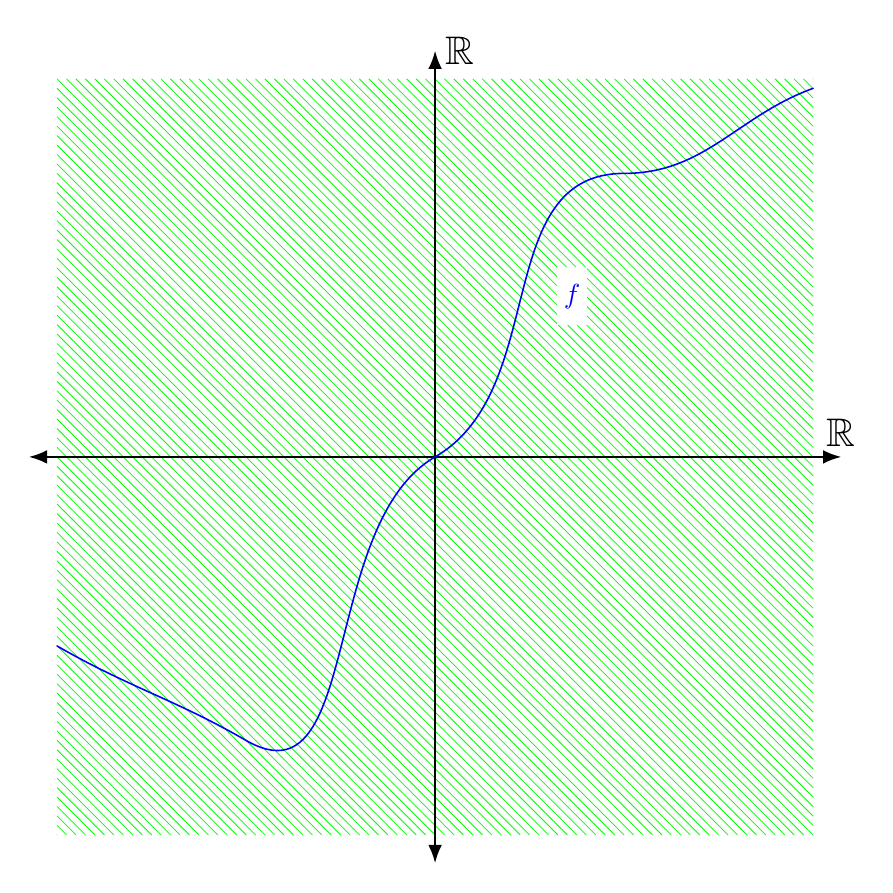
\begin{tikzpicture}[%
    >=Latex,
    line width=0.2mm,
    line cap=round,
    scale=1.2
]
    % Coorindates for the curve.
    \coordinate (P1) at (-4.00, -2.00);
    \coordinate (P2) at (-2.00, -3.00);
    \coordinate (P3) at ( 0.00,  0.00);
    \coordinate (P4) at ( 2.00,  3.00);
    \coordinate (P5) at ( 4.00,  3.90);

    % Draw a green mesh indicating the Cartesian plane.
    \foreach\x in {-40, -39, ..., 39}{
        \draw[draw=green, line width=0.1mm] (\x/10, -4) to (-4, \x/10);
        \draw[draw=green, line width=0.1mm] (4, \x/10)  to (\x/10, 4);
    }
    \draw[draw=green, line width=0.1mm] (4, 4)  to (4, 4);

    \begin{scope}[thick, font=\Large]
        \draw[<->] (-4.3,  0.0) to (4.3, 0.0) node [above] {$\mathbb{R}$};
        \draw[<->] ( 0.0, -4.3) to (0.0, 4.3) node [right] {$\mathbb{R}$};
    \end{scope}

    \draw[draw=blue] (P1) to [out=-30, in=150]  (P2)
                          to [out=-30, in=210]  (P3)
                          to [out=30,  in=180]  (P4)
                          to [out=0,   in=200]  (P5);
    \draw[fill=white, draw=white] 
        (1.3, 2.0) rectangle node {$\textcolor{blue}{f}$} (1.6, 1.4);
\end{tikzpicture}
            \caption[Example of a Function
                     $f:\mathbb{R}\rightarrow\mathbb{R}$]
                    {Example of a function
                     $f:\mathbb{R}\rightarrow\mathbb{R}$.
                     The Cartesian product $\mathbb{R}\times\mathbb{R}$ is
                     shown in \textcolor{green!80!black}{green}, and the
                     function $f\subseteq\mathbb{R}\times\mathbb{R}$ is shown
                     in \textcolor{blue}{blue}.}
            \label{fig:Function_R_to_R_Subset_Cart_Prod}
        \end{figure}
        \begin{lexample}{}{SQRT_is_Not_a_Function}
            Let $g\subseteq\mathbb{R}\times\mathbb{R}$ be defined as follows:
            \begin{equation}
                g=\big\{\;(x,y)\in\mathbb{R}^{2}\,:\,y^{2}=x\;\big\}
            \end{equation}
            It is tempting to label $g$ by writing $g(x)=\sqrt{x}$, but $g$ is
            not a function for it fails two of the requirements of a function.
            Firstly, for any $x>0$, there are two values $y_{1}$ and $y_{2}$
            whose square is equal to $x$. Indeed, if $y_{1}$ is one such value,
            then setting $y_{2}=\minus{y}_{1}$ will result in a second
            distinct value. Thus $g$ does not have the uniqueness property
            required for functions. Moreover, if $x<0$, then there is no such
            value $y\in\mathbb{R}$ such that $(x,y)\in{g}$, and thus $g$ also
            lacks the existence property. In terms of the vertical line test,
            there are points $x$ such that the vertical line through
            $(x,\,0)$ intersects $g$ twice, and there are points such that the
            vertical line does not intersect at all. The graph of $g$ is shown
            in Fig.~\ref{fig:SQRT_Not_a_Function}.
        \end{lexample}
        We need not only consider functions of the for
        $f:\mathbb{R}\rightarrow\mathbb{R}$, nor functions
        $f:\mathcal{U}\rightarrow\mathcal{V}$, where $\mathcal{U}$ and
        $\mathcal{V}$ are subsets of $\mathbb{R}$, and we can allow for
        arbitrary abstract functions.
        \begin{figure}[H]
            \centering
            %--------------------------------Dependencies----------------------------------%
%   xcolor                                                                     %
%   amssymb                                                                    %
%   tikz                                                                       %
%       arrows.meta                                                            %
%       patterns                                                               %
%-------------------------------Main Document----------------------------------%
\begin{tikzpicture}[%
    >=Latex,
    line width=0.2mm,
    line cap=round,
    scale=1.2
]
    % Coorindates for the curve.
    \coordinate (P1) at (-3.85, -2.00);
    \coordinate (P2) at (-2.00, -3.00);
    \coordinate (P3) at ( 0.00,  0.00);
    \coordinate (P4) at ( 2.00,  3.00);
    \coordinate (P5) at ( 3.85,  3.80);

    \draw[%
        pattern=north west lines,
        pattern color=Green!80!Black,
        opacity=0.5,
        draw=white
    ]   (-3.9, -3.9) rectangle (3.9, 3.9);

    \begin{scope}[thick, font=\Large]
        \draw[<->] (-4.2, 0) to (4.2, 0) node [above] {$\mathbb{R}$};
        \draw[<->] (0, -4.2) to (0, 4.2) node [right] {$\mathbb{R}$};
    \end{scope}

    \draw[draw=red] (3.880000, -1.969772) to (3.840000, -1.959592)
                                          to (3.800000, -1.949359)
                                          to (3.760000, -1.939072)
                                          to (3.720000, -1.928730)
                                          to (3.680000, -1.918333)
                                          to (3.640000, -1.907878)
                                          to (3.600000, -1.897367)
                                          to (3.560000, -1.886796)
                                          to (3.520000, -1.876166)
                                          to (3.480000, -1.865476)
                                          to (3.440000, -1.854724)
                                          to (3.400000, -1.843909)
                                          to (3.360000, -1.833030)
                                          to (3.320000, -1.822087)
                                          to (3.280000, -1.811077)
                                          to (3.240000, -1.800000)
                                          to (3.200000, -1.788854)
                                          to (3.160000, -1.777639)
                                          to (3.120000, -1.766352)
                                          to (3.080000, -1.754993)
                                          to (3.040000, -1.743560)
                                          to (3.000000, -1.732051)
                                          to (2.960000, -1.720465)
                                          to (2.920000, -1.708801)
                                          to (2.880000, -1.697056)
                                          to (2.840000, -1.685230)
                                          to (2.800000, -1.673320)
                                          to (2.760000, -1.661325)
                                          to (2.720000, -1.649242)
                                          to (2.680000, -1.637071)
                                          to (2.640000, -1.624808)
                                          to (2.600000, -1.612452)
                                          to (2.560000, -1.600000)
                                          to (2.520000, -1.587451)
                                          to (2.480000, -1.574802)
                                          to (2.440000, -1.562050)
                                          to (2.400000, -1.549193)
                                          to (2.360000, -1.536229)
                                          to (2.320000, -1.523155)
                                          to (2.280000, -1.509967)
                                          to (2.240000, -1.496663)
                                          to (2.200000, -1.483240)
                                          to (2.160000, -1.469694)
                                          to (2.120000, -1.456022)
                                          to (2.080000, -1.442221)
                                          to (2.040000, -1.428286)
                                          to (2.000000, -1.414214)
                                          to (1.960000, -1.400000)
                                          to (1.920000, -1.385641)
                                          to (1.880000, -1.371131)
                                          to (1.840000, -1.356466)
                                          to (1.800000, -1.341641)
                                          to (1.760000, -1.326650)
                                          to (1.720000, -1.311488)
                                          to (1.680000, -1.296148)
                                          to (1.640000, -1.280625)
                                          to (1.600000, -1.264911)
                                          to (1.560000, -1.249000)
                                          to (1.520000, -1.232883)
                                          to (1.480000, -1.216553)
                                          to (1.440000, -1.200000)
                                          to (1.400000, -1.183216)
                                          to (1.360000, -1.166190)
                                          to (1.320000, -1.148913)
                                          to (1.280000, -1.131371)
                                          to (1.240000, -1.113553)
                                          to (1.200000, -1.095445)
                                          to (1.160000, -1.077033)
                                          to (1.120000, -1.058301)
                                          to (1.080000, -1.039230)
                                          to (1.040000, -1.019804)
                                          to (1.000000, -1.000000)
                                          to (0.960000, -0.979796)
                                          to (0.920000, -0.959166)
                                          to (0.880000, -0.938083)
                                          to (0.840000, -0.916515)
                                          to (0.800000, -0.894427)
                                          to (0.760000, -0.871780)
                                          to (0.720000, -0.848528)
                                          to (0.680000, -0.824621)
                                          to (0.640000, -0.800000)
                                          to (0.600000, -0.774597)
                                          to (0.560000, -0.748331)
                                          to (0.520000, -0.721110)
                                          to (0.480000, -0.692820)
                                          to (0.440000, -0.663325)
                                          to (0.400000, -0.632456)
                                          to (0.360000, -0.600000)
                                          to (0.320000, -0.565685)
                                          to (0.280000, -0.529150)
                                          to (0.240000, -0.489898)
                                          to (0.200000, -0.447214)
                                          to (0.160000, -0.400000)
                                          to (0.120000, -0.346410)
                                          to (0.080000, -0.282843)
                                          to (0.040000, -0.200000)
                                          to (0.000000, 0.000000) 
                                          to (0.040000, 0.200000)
                                          to (0.080000, 0.282843)
                                          to (0.120000, 0.346410)
                                          to (0.160000, 0.400000)
                                          to (0.200000, 0.447214)
                                          to (0.240000, 0.489898)
                                          to (0.280000, 0.529150)
                                          to (0.320000, 0.565685)
                                          to (0.360000, 0.600000)
                                          to (0.400000, 0.632456)
                                          to (0.440000, 0.663325)
                                          to (0.480000, 0.692820)
                                          to (0.520000, 0.721110)
                                          to (0.560000, 0.748331)
                                          to (0.600000, 0.774597)
                                          to (0.640000, 0.800000)
                                          to (0.680000, 0.824621)
                                          to (0.720000, 0.848528)
                                          to (0.760000, 0.871780)
                                          to (0.800000, 0.894427)
                                          to (0.840000, 0.916515)
                                          to (0.880000, 0.938083)
                                          to (0.920000, 0.959166)
                                          to (0.960000, 0.979796)
                                          to (1.000000, 1.000000)
                                          to (1.040000, 1.019804)
                                          to (1.080000, 1.039230)
                                          to (1.120000, 1.058301)
                                          to (1.160000, 1.077033)
                                          to (1.200000, 1.095445)
                                          to (1.240000, 1.113553)
                                          to (1.280000, 1.131371)
                                          to (1.320000, 1.148913)
                                          to (1.360000, 1.166190)
                                          to (1.400000, 1.183216)
                                          to (1.440000, 1.200000)
                                          to (1.480000, 1.216553)
                                          to (1.520000, 1.232883)
                                          to (1.560000, 1.249000)
                                          to (1.600000, 1.264911)
                                          to (1.640000, 1.280625)
                                          to (1.680000, 1.296148)
                                          to (1.720000, 1.311488)
                                          to (1.760000, 1.326650)
                                          to (1.800000, 1.341641)
                                          to (1.840000, 1.356466)
                                          to (1.880000, 1.371131)
                                          to (1.920000, 1.385641)
                                          to (1.960000, 1.400000)
                                          to (2.000000, 1.414214)
                                          to (2.040000, 1.428286)
                                          to (2.080000, 1.442221)
                                          to (2.120000, 1.456022)
                                          to (2.160000, 1.469694)
                                          to (2.200000, 1.483240)
                                          to (2.240000, 1.496663)
                                          to (2.280000, 1.509967)
                                          to (2.320000, 1.523155)
                                          to (2.360000, 1.536229)
                                          to (2.400000, 1.549193)
                                          to (2.440000, 1.562050)
                                          to (2.480000, 1.574802)
                                          to (2.520000, 1.587451)
                                          to (2.560000, 1.600000)
                                          to (2.600000, 1.612452)
                                          to (2.640000, 1.624808)
                                          to (2.680000, 1.637071)
                                          to (2.720000, 1.649242)
                                          to (2.760000, 1.661325)
                                          to (2.800000, 1.673320)
                                          to (2.840000, 1.685230)
                                          to (2.880000, 1.697056)
                                          to (2.920000, 1.708801)
                                          to (2.960000, 1.720465)
                                          to (3.000000, 1.732051)
                                          to (3.040000, 1.743560)
                                          to (3.080000, 1.754993)
                                          to (3.120000, 1.766352)
                                          to (3.160000, 1.777639)
                                          to (3.200000, 1.788854)
                                          to (3.240000, 1.800000)
                                          to (3.280000, 1.811077)
                                          to (3.320000, 1.822087)
                                          to (3.360000, 1.833030)
                                          to (3.400000, 1.843909)
                                          to (3.440000, 1.854724)
                                          to (3.480000, 1.865476)
                                          to (3.520000, 1.876166)
                                          to (3.560000, 1.886796)
                                          to (3.600000, 1.897367)
                                          to (3.640000, 1.907878)
                                          to (3.680000, 1.918333)
                                          to (3.720000, 1.928730)
                                          to (3.760000, 1.939072)
                                          to (3.800000, 1.949359)
                                          to (3.840000, 1.959592)
                                          to (3.880000, 1.969772);
    \draw[fill=white, draw=white] 
        (1.3, 2.0) rectangle node {$\textcolor{red}{g}$} (1.6, 1.5);
\end{tikzpicture}
            \caption[Example of a Non-Function]
                {$g\subseteq\mathbb{R}\times\mathbb{R}$ is not a function
                 since it fails the vertical line test.}
            \label{fig:SQRT_Not_a_Function}
        \end{figure}
        \begin{lexample}{Abstract Functions}{Abstract_Functions}
            Let $A$ and $B$ be sets defined as follows:
            \par
            \begin{subequations}
                \begin{minipage}[b]{0.49\textwidth}
                    \centering
                    \begin{equation}
                        A=\{\,1,\,2,\,3,\,4\,\}
                    \end{equation}
                \end{minipage}
                \hfill
                \begin{minipage}[b]{0.49\textwidth}
                    \centering
                    \begin{equation}
                        B=\{\,a,\,b,\,c\,\}
                    \end{equation}
                \end{minipage}
            \end{subequations}
            \par\vspace{2.5ex}
            Similar to the vertical line test, we can devise a visual to
            discerning functions from non-functions for abstract sets.
            We represents the elements of $A$ and $B$ as points in some blob
            in the plane, and then draw arrows between the points
            $x\in{A}$ and $y\in{b}$ indicating that $(x,\,y)\in{f}$.
            This allows us to discern between functions and non-functions.
            Every point in $A$ must be mapped to a unique point in $B$.
            That is, every point in $A$ must have one and only one arrow
            connecting it to some point in $B$. Examples of valid functions
            are shown in Fig.~\ref{fig:Abstract_Functions}, and non-functions
            are shown in Fig.~\ref{fig:Abstract_Non_Functions}.
        \end{lexample}
        \begin{figure}[H]
            \centering
            \begin{subfigure}[b]{0.49\textwidth}
                \centering
                \resizebox{\textwidth}{!}{%
                    %--------------------------------Dependencies----------------------------------%
%   tikz                                                                       %
%       arrows.meta                                                            %
%-------------------------------Main Document----------------------------------%
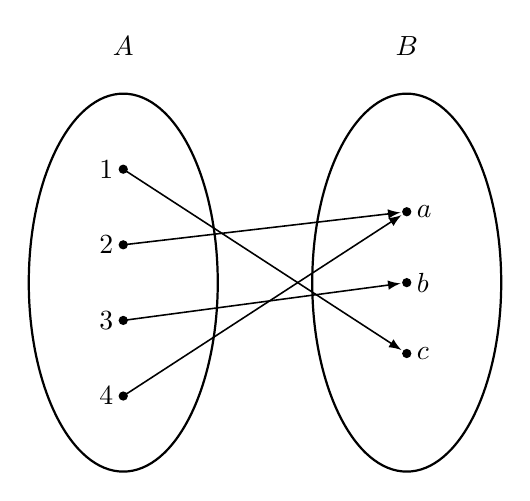
\begin{tikzpicture}[%
    >=latex,
    line width=0.2mm,
    line cap=round,
    scale=1.2
]
    % Coorindates.
    \coordinate (a) at ( 1.5,  0.75);
    \coordinate (b) at ( 1.5, -0.00);
    \coordinate (c) at ( 1.5, -0.75);
    \coordinate (1) at (-1.5,  1.20);
    \coordinate (2) at (-1.5,  0.40);
    \coordinate (3) at (-1.5, -0.40);
    \coordinate (4) at (-1.5, -1.20);
    \coordinate (A) at (-1.5,  2.50);
    \coordinate (B) at ( 1.5,  2.50);

    % Ellipses representing the sets A and B.
    \draw[thick] (-1.5, 0.0) ellipse (1 and 2);
    \draw[thick] ( 1.5, 0.0) ellipse (1 and 2);

    % Draw circles for the various points.
    \draw[fill=black] (a) circle (0.4mm);
    \draw[fill=black] (b) circle (0.4mm);
    \draw[fill=black] (c) circle (0.4mm);
    \draw[fill=black] (1) circle (0.4mm);
    \draw[fill=black] (2) circle (0.4mm);
    \draw[fill=black] (3) circle (0.4mm);
    \draw[fill=black] (4) circle (0.4mm);

    % Draw paths indicating mappings.
    \begin{scope}[->]
        \draw[shorten >=0.8mm] (1) to (c);
        \draw[shorten >=0.8mm] (2) to (a);
        \draw[shorten >=0.8mm] (3) to (b);
        \draw[shorten >=0.8mm] (4) to (a);
    \end{scope}

    % Labels.
    \node at (A)         {$A$};
    \node at (B)         {$B$};
    \node at (a) [right] {$a$};
    \node at (b) [right] {$b$};
    \node at (c) [right] {$c$};
    \node at (1) [left]  {$1$};
    \node at (2) [left]  {$2$};
    \node at (3) [left]  {$3$};
    \node at (4) [left]  {$4$};
\end{tikzpicture}
                }
                \subcaption{A Valid Function.}
            \end{subfigure}
            \begin{subfigure}[b]{0.49\textwidth}
                \centering
                \resizebox{\textwidth}{!}{%
                    %--------------------------------Dependencies----------------------------------%
%   tikz                                                                       %
%       arrows.meta                                                            %
%-------------------------------Main Document----------------------------------%
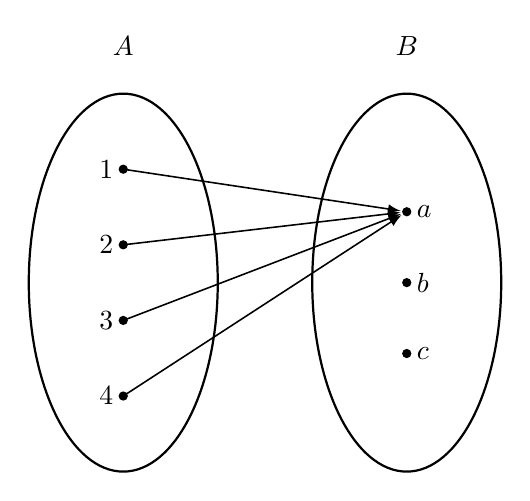
\begin{tikzpicture}[%
    >=latex,
    line width=0.2mm,
    line cap=round,
    scale=1.2
]
    % Coorindates.
    \coordinate (a) at ( 1.5,  0.75);
    \coordinate (b) at ( 1.5, -0.00);
    \coordinate (c) at ( 1.5, -0.75);
    \coordinate (1) at (-1.5,  1.20);
    \coordinate (2) at (-1.5,  0.40);
    \coordinate (3) at (-1.5, -0.40);
    \coordinate (4) at (-1.5, -1.20);
    \coordinate (A) at (-1.5,  2.50);
    \coordinate (B) at ( 1.5,  2.50);

    % Ellipses representing the sets A and B.
    \draw[thick] (-1.5, 0.0) ellipse (1 and 2);
    \draw[thick] ( 1.5, 0.0) ellipse (1 and 2);

    % Draw circles for the various points.
    \draw[fill=black] (a) circle (0.4mm);
    \draw[fill=black] (b) circle (0.4mm);
    \draw[fill=black] (c) circle (0.4mm);
    \draw[fill=black] (1) circle (0.4mm);
    \draw[fill=black] (2) circle (0.4mm);
    \draw[fill=black] (3) circle (0.4mm);
    \draw[fill=black] (4) circle (0.4mm);

    % Draw paths indicating mappings.
    \begin{scope}[->]
        \draw[shorten >=0.8mm] (1) to (a);
        \draw[shorten >=0.8mm] (2) to (a);
        \draw[shorten >=0.8mm] (3) to (a);
        \draw[shorten >=0.8mm] (4) to (a);
    \end{scope}

    % Labels.
    \node at (A)         {$A$};
    \node at (B)         {$B$};
    \node at (a) [right] {$a$};
    \node at (b) [right] {$b$};
    \node at (c) [right] {$c$};
    \node at (1) [left]  {$1$};
    \node at (2) [left]  {$2$};
    \node at (3) [left]  {$3$};
    \node at (4) [left]  {$4$};
\end{tikzpicture}
                }
                \subcaption{Another Valid Function.}
            \end{subfigure}
            \caption{Visual for Abstract Functions}
            \label{fig:Abstract_Functions}
        \end{figure}
        \begin{figure}[H]
            \centering
            \begin{subfigure}[b]{0.49\textwidth}
                \centering
                \resizebox{\textwidth}{!}{%
                    %--------------------------------Dependencies----------------------------------%
%   tikz                                                                       %
%       arrows.meta                                                            %
%-------------------------------Main Document----------------------------------%
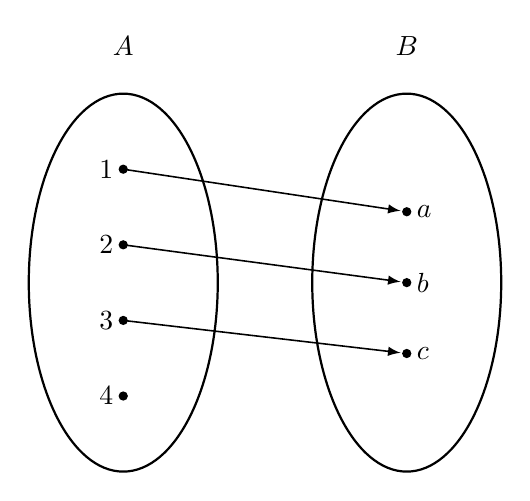
\begin{tikzpicture}[%
    >=latex,
    line width=0.2mm,
    line cap=round,
    scale=1.2
]
    % Coorindates.
    \coordinate (a) at ( 1.5,  0.75);
    \coordinate (b) at ( 1.5, -0.00);
    \coordinate (c) at ( 1.5, -0.75);
    \coordinate (1) at (-1.5,  1.20);
    \coordinate (2) at (-1.5,  0.40);
    \coordinate (3) at (-1.5, -0.40);
    \coordinate (4) at (-1.5, -1.20);
    \coordinate (A) at (-1.5,  2.50);
    \coordinate (B) at ( 1.5,  2.50);

    % Ellipses representing the sets A and B.
    \draw[thick] (-1.5, 0.0) ellipse (1 and 2);
    \draw[thick] ( 1.5, 0.0) ellipse (1 and 2);

    % Draw circles for the various points.
    \draw[fill=black] (a) circle (0.4mm);
    \draw[fill=black] (b) circle (0.4mm);
    \draw[fill=black] (c) circle (0.4mm);
    \draw[fill=black] (1) circle (0.4mm);
    \draw[fill=black] (2) circle (0.4mm);
    \draw[fill=black] (3) circle (0.4mm);
    \draw[fill=black] (4) circle (0.4mm);

    % Draw paths indicating mappings.
    \begin{scope}[->]
        \draw[shorten >=0.8mm] (1) to (a);
        \draw[shorten >=0.8mm] (2) to (b);
        \draw[shorten >=0.8mm] (3) to (c);
    \end{scope}

    % Labels.
    \node at (A)         {$A$};
    \node at (B)         {$B$};
    \node at (a) [right] {$a$};
    \node at (b) [right] {$b$};
    \node at (c) [right] {$c$};
    \node at (1) [left]  {$1$};
    \node at (2) [left]  {$2$};
    \node at (3) [left]  {$3$};
    \node at (4) [left]  {$4$};
\end{tikzpicture}
                }
                \subcaption{Fails Existence.}
            \end{subfigure}
            \begin{subfigure}[b]{0.49\textwidth}
                \centering
                \resizebox{\textwidth}{!}{%
                    %--------------------------------Dependencies----------------------------------%
%   tikz                                                                       %
%       arrows.meta                                                            %
%-------------------------------Main Document----------------------------------%
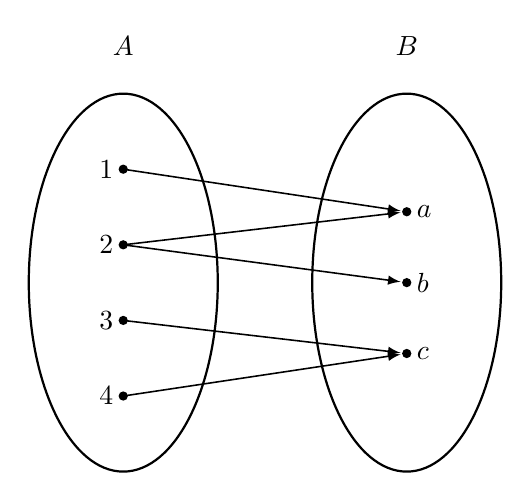
\begin{tikzpicture}[%
    >=latex,
    line width=0.2mm,
    line cap=round,
    scale=1.2
]
    % Coorindates.
    \coordinate (a) at ( 1.5,  0.75);
    \coordinate (b) at ( 1.5, -0.00);
    \coordinate (c) at ( 1.5, -0.75);
    \coordinate (1) at (-1.5,  1.20);
    \coordinate (2) at (-1.5,  0.40);
    \coordinate (3) at (-1.5, -0.40);
    \coordinate (4) at (-1.5, -1.20);
    \coordinate (A) at (-1.5,  2.50);
    \coordinate (B) at ( 1.5,  2.50);

    % Ellipses representing the sets A and B.
    \draw[thick] (-1.5, 0.0) ellipse (1 and 2);
    \draw[thick] ( 1.5, 0.0) ellipse (1 and 2);

    % Draw circles for the various points.
    \draw[fill=black] (a) circle (0.4mm);
    \draw[fill=black] (b) circle (0.4mm);
    \draw[fill=black] (c) circle (0.4mm);
    \draw[fill=black] (1) circle (0.4mm);
    \draw[fill=black] (2) circle (0.4mm);
    \draw[fill=black] (3) circle (0.4mm);
    \draw[fill=black] (4) circle (0.4mm);

    % Draw paths indicating mappings.
    \begin{scope}[->]
        \draw[shorten >=0.8mm] (1) to (a);
        \draw[shorten >=0.8mm] (2) to (a);
        \draw[shorten >=0.8mm] (2) to (b);
        \draw[shorten >=0.8mm] (3) to (c);
        \draw[shorten >=0.8mm] (4) to (c);
    \end{scope}

    % Labels.
    \node at (A)         {$A$};
    \node at (B)         {$B$};
    \node at (a) [right] {$a$};
    \node at (b) [right] {$b$};
    \node at (c) [right] {$c$};
    \node at (1) [left]  {$1$};
    \node at (2) [left]  {$2$};
    \node at (3) [left]  {$3$};
    \node at (4) [left]  {$4$};
\end{tikzpicture}
                }
                \subcaption{Fails Uniqueness.}
            \end{subfigure}
            \caption{Non-Functions}
            \label{fig:Abstract_Non_Functions}
        \end{figure}
        Looking at the sets in Ex.\ref{ex:Abstract_Functions}, it is possible
        to count the total number of functions from $A$ to $B$. Since every
        element of $A$ needs to be mapped to some element of $B$, and since
        there are 4 elements in $A$ and 3 elements in $B$, the total number of
        functions $f:A\rightarrow{B}$ is $4^{3}=64$. On the other hand, the
        total number of subsets of $A\times{B}$ is $2^{12}=4096$
        (We will justify this when we discuss the \textit{cardinality} of
        sets). Thus, if we were to randomly pick a subset of $A\times{B}$, the
        odds are that it is almost certainly \textit{not} a function
        (1.5625\%).
        \begin{ldefinition}{Image of a Point}{Image_of_Point}
            The image of an element $x$ in a set $A$ under a
            function $f:A\rightarrow{B}$ is the unique value
            $y\in{B}$ such that $(x,y)\in{f}$. We denote this
            by writing $y=f(x)$.
        \end{ldefinition}
        Similarly, we can define the image of an entire subset.
        \begin{ldefinition}{Image of a Subset}{Image_of_Subset}
            The image of a subset $\mathcal{U}$ of a set $A$
            under a function $f:A\rightarrow{B}$ is the set:
            \begin{equation}
                f\big(\mathcal{U}\big)=
                    \{\;f(x)\,:\,x\in\mathcal{U}\;\}
            \end{equation}
            That is, the set of all points in $B$ that are the
            image of points in $\mathcal{U}$ under $f$.
        \end{ldefinition}
        This is also called the \textit{range} of a function.
        In a similar manner, we can define the pre-image, or
        inverse image, of a set.
    \subsection{Basic Theorems}
        \begin{theorem}
            \label{thm:Emptyset_Is_Subset}%
            If $A$ is a set, then $\emptyset\subseteq{A}$.
        \end{theorem}
        \begin{proof}
            For suppose not. Then there is an $x\in\emptyset$
            such that $x\notin{A}$, a contradiction as
            for all $x$, it is true that $x\notin\emptyset$
            (Def.~\ref{def:Empty_Set}). Therefore, etc.
        \end{proof}
        \begin{theorem}
            \label{thm:Subset_is_Transitive}%
            If $A$, $B$, and $C$ are sets, if
            $A\subseteq{B}$, and if $B\subseteq{C}$, then
            $A\subseteq{C}$.
        \end{theorem}
        \begin{proof}
            For suppose not. Then there is an $x\in{A}$ such
            that $x\notin{C}$. But $A$ is a subset of $B$
            and thus $x\in{B}$ (Def.~\ref{def:Subsets}). But
            $B$ is a subset of $C$ and therefore $x\in{C}$
            (Def.~\ref{def:Subsets}). But $x\notin{C}$, a
            contradiction. Therefore, etc.
        \end{proof}
        \begin{theorem}
            \label{thm:Set_Is_Subset_Of_Self}%
            If $A$ is a set, then $A\subseteq{A}$.
        \end{theorem}
        \begin{proof}
            Suppose not. Then there is an $x\in{A}$
            such that $x\notin{A}$, a contradiction.
        \end{proof}
        We write $A\ne{B}$ to denote that $A$ and $B$ are
        not equal sets. From the definition, we have
        inequality when either $A\nsubseteq{B}$ or
        $B\nsubseteq{A}$.
        We can now rigorously restate our claim that the
        empty set is unique.
        \begin{theorem}
            If $\emptyset'$ is a set with no elements,
            then $\emptyset=\emptyset'$.
        \end{theorem}
        \begin{proof}
            For suppose not. But $\emptyset'$ is a set, and
            thus $\emptyset\subseteq\emptyset'$
            (Thm.~\ref{thm:Emptyset_Is_Subset}). Therefore
            $\emptyset'\nsubseteq\emptyset$. But then there
            is an $x$ such that $x\in\emptyset'$ and
            $x\notin\emptyset$. But $\emptyset'$ contains
            no elements, a contradiction. Thus
            $\emptyset'\subseteq\emptyset$. Therefore,
            $\emptyset=\emptyset'$
            (Def.~\ref{def:Equal_Sets}).
        \end{proof}
        \begin{theorem}
            \label{thm:Subsets_of_Equal_Sets}%
            If $A$, $B$, and $C$ are sets, if $A=B$, and if
            $C\subseteq{A}$, then $C\subseteq{B}$.
        \end{theorem}
        \begin{proof}
            For if $A=B$, then $A\subseteq{B}$
            (Def.~\ref{def:Equal_Sets}). But if
            $C\subseteq{A}$ and $A\subseteq{B}$, then
            $C\subseteq{B}$
            (Thm.~\ref{thm:Subset_is_Transitive}).
            Therefore, etc.
        \end{proof}
        \begin{theorem}
            \label{thm:Equality_Symmetric}%
            If $A$ and $B$ are equal sets, then $B$ and
            $A$ are equal sets.
        \end{theorem}
        \begin{proof}
            For suppose not. If $B\ne{A}$, then either
            $B\nsubseteq{A}$ or $A\nsubseteq{B}$.
            But $A=B$, and thus $A\subseteq{B}$  and
            $B\subseteq{A}$ (Def.~\ref{def:Equal_Sets}),
            a contradiction. Therefore, etc.
        \end{proof}
        \begin{theorem}
            \label{thm:Equality_Reflexive}%
            If $A$ is a set, then $A=A$.
        \end{theorem}
        \begin{proof}
            For if $A$ is a set then $A\subseteq{A}$
            (Thm.~\ref{thm:Set_Is_Subset_Of_Self}).
            Therefore, etc.
        \end{proof}
        \begin{theorem}
            \label{thm:Equality_Transitive}%
            If $A$, $B$, and $C$ are sets, if $A=B$, and if
            $B=C$, then $A=C$.
        \end{theorem}
        \begin{proof}
            For if $B=C$, then $C\subseteq{B}$ (Def.~\ref{def:Equal_Sets}).
            But if $A=B$, then $B=A$ (Thm.~\ref{thm:Equality_Symmetric}). But
            if $B=A$ and and $C\subseteq{B}$, then $C\subseteq{A}$
            (Thm.~\ref{thm:Subsets_of_Equal_Sets}). And if $A=B$, then
            $A\subseteq{B}$ (Def.~\ref{def:Equal_Sets}). But if $B=C$ and
            $A\subseteq{B}$, then $A\subseteq{C}$
            (Thm.~\ref{thm:Subsets_of_Equal_Sets}). But it was just proved
            that $C\subseteq{A}$, and thus $A=C$ (Def.~\ref{def:Equal_Sets}).
            Therefore, etc.
        \end{proof}
        These three properties,
        Thms.~\ref{thm:Equality_Reflexive}-%
        \ref{thm:Equality_Transitive}, are the key
        ingredients to define \textit{equivalence relations}.
        \begin{theorem}
            \label{thm:Prop_Subset_Not_Equal}%
            If $A$ and $B$ are sets, and if $A$ is a proper
            subset of $B$, then there is an $x\in{B}$ such
            that $x\notin{A}$.
        \end{theorem}
        \begin{proof}
            For suppose not. Then for all $x\in{B}$,
            it is true that $x\in{A}$. But then
            $B$ is a subset of $A$ (Def.~\ref{def:Subsets}).
            But $A$ is a subset of $B$, and thus $A=B$
            (Def.~\ref{def:Equal_Sets}), a contradiction as
            $A$ is a proper subset. Therefore, etc.
        \end{proof}
        Theorem \ref{thm:Prop_Subset_Not_Equal} can
        be used as an equivalent definition of a proper
        subset. That is, a proper subset is a subset that
        is missing at least one element.
        \section{Operations on Sets}
        Similar to the arithmetic of real numbers, there
        are standard operations that can be performed on
        sets to obtain new sets. The four most common
        operations are union, intersection, set difference,
        and symmetric difference. Often the
        \textit{complement} of a set is discussed, but as
        we will see, this is just a specific case of set
        difference.
        \begin{figure}[H]
            \centering
            %--------------------------------Dependencies----------------------------------%
%   tikz                                                                       %
%-------------------------------Main Document----------------------------------%
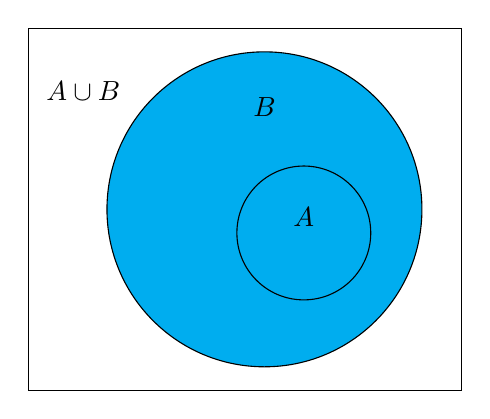
\begin{tikzpicture}
    \draw (-3,-2.3) rectangle (2.5,2.3);
    \draw[fill=cyan] (0,0) circle (2);
    \draw (0.5,-0.3) circle (0.85);
    \node at (0.5,-0.1) {$A$};
    \node at (0,1.3) {$B$};
    \node at (-2.3,1.5) {$A\cup{B}$};
\end{tikzpicture}
            \caption{Visual for Thm.~\ref{thm:Union_With_Subset}.}
            \label{fig:Venn_Diagram_Union_With_Subset}
        \end{figure}
        Set operations are very algebraic, and it is often
        useful to build up several small tools to eventually
        prove larger theorems in a simple way. We wish to
        show that union is commutative and associative, and
        that there is an \textit{identity}.
        \begin{ltheorem}{Commutative Law of Unions}{Commutative_Law_of_Unions}
            If $A$ and $B$ are sets, then $A\cup{B}=B\cup{A}$.
        \end{ltheorem}
        \begin{proof}
            For if $x\in{A}\cup{B}$, then either $x\in{A}$ or $x\in{B}$, or
            both (Def.~\ref{def:Union_of_Two}). But then either $x\in{B}$ or
            $x\in{A}$, or both, and therefore $x\in{B}\cup{A}$
            (Def.~\ref{def:Union_of_Two}). But then for all $x\in{A}\cup{B}$
            it is true that $x\in{B}\cup{A}$, and therefore
            $A\cup{B}\subseteq{B}\cup{A}$ (Def.~\ref{def:Subsets}). Similarly,
            $B\cup{A}\subseteq{A}\cup{B}$, and thus $A\cup{B}=B\cup{A}$
            (Def.~\ref{def:Equal_Sets}). Therefore, etc.
        \end{proof}
        When taking the union of two sets, we obtain a
        \textit{larger} set, in a sense. Again relying on
        the analogy of arithmetic, given two non-negative
        integers $a$ and $b$, it is true that $a\leq{a}+b$.
        Equality is obtained if and only if either $a$ or
        $b$ is equal to zero. As we will see, the empty set
        acts as the \textit{zero} of unions. Also, given
        three non-negative integers $a$, $b$, and $c$, if
        $b\leq{c}$, then $a+b\leq{a}+c$. A similar result
        will hold for sets and unions.
        \begin{theorem}
            \label{thm:Union_is_Bigger}%
            If $A$ and $B$ are sets, then
            $A\subseteq{A}\cup{B}$.
        \end{theorem}
        \begin{proof}
            For suppose not. Then there is an $x\in{A}$ such
            that $x\notin{A}\cup{B}$. But if $x\in{A}$, then
            $x\in{A}$ or $x\in{B}$ and thus $x\in{A}\cup{B}$
            (Def.~\ref{def:Union_of_Two}), a
            contradiction. Therefore, etc.
        \end{proof}
        \begin{theorem}
            \label{thm:Union_With_Lesser_Set}%
            If $A$, $B$, and $C$ are sets, and if
            $B\subseteq{C}$, then
            $A\cup{B}\subseteq{A}\cup{C}$.
        \end{theorem}
        \begin{proof}
            For if $x\in{A}\cup{B}$, then either $x\in{A}$,
            or $x\in{B}$, or both
            (Def.~\ref{def:Union_of_Two}). But $B$ is a
            subset of $C$, and therefore if $x\in{B}$, then
            $x\in{C}$ (Def.~\ref{def:Subsets}).
            Thus, if $x\in{A}$ or $x\in{B}$, then
            $x\in{A}$ or $x\in{C}$, and therefore
            $x\in{A}\cup{C}$ (Def.~\ref{def:Union_of_Two}).
            Thus, $A\cup{B}\subseteq{A}\cup{C}$
            (Def.~\ref{def:Subsets}). Therefore, etc.
        \end{proof}
        \begin{theorem}
            If $A$, $B$, $C$, and $D$ are sets, if
            $A\subseteq{C}$, and if $B\subseteq{D}$, then
            $A\cup{B}\subseteq{C}\cup{D}$.
        \end{theorem}
        \begin{proof}
            For if $B\subseteq{D}$, then
            $A\cup{B}\subseteq{A}\cup{D}$
            (Thm.~\ref{thm:Union_With_Lesser_Set}).
            But $A\cup{D}=D\cup{A}$
            (Thm.~\ref{thm:Commutative_Law_of_Unions}).
            But if $A\subseteq{C}$, then
            $D\cup{A}\subseteq{D}\cup{C}$
            (Thm.~\ref{thm:Union_With_Lesser_Set}). But
            $D\cup{C}=C\cup{D}$
            (Thm.~\ref{thm:Commutative_Law_of_Unions}).
            And if $A\cup{B}\subseteq{A}\cup{D}$ and
            $A\cup{D}\subseteq{C}\cup{D}$, then
            $A\cup{B}\subseteq{C}\cup{D}$
            (Thm.~\ref{thm:Subset_is_Transitive}).
            Therefore, etc.
        \end{proof}
        Taking the union of subsets is redundant, as we
        simply obtain the larger set. This starts to break
        down the analogy between sets and arithmetic, since
        there is only one \textit{zero}. That is, there is
        only one number $b$ such that $a+b=a$, and that is
        $b=0$. While any subset acts as a \textit{zero} of a
        given set, the empty set has the property that it
        acts as a zero for \textit{every} set. It is the only
        set with this property, and thus the analogy with
        arithmetic is restored.
        \begin{theorem}
            \label{thm:Union_With_Subset}%
            If $A$ and $B$ are sets, and if
            $A\subseteq{B}$, then $A\cup{B}=B$.
        \end{theorem}
        \begin{proof}
            For if $A$ and $B$ are sets, then
            $B\subseteq{A}\cup{B}$
            (Thm.~\ref{thm:Union_is_Bigger}).
            But if $A\subseteq{B}$, then for all $x\in{A}$,
            it is true that $x\in{B}$
            (Def.~\ref{def:Subsets}). Thus if $x\in{A}$ or if
            $x\in{B}$, then $x\in{B}$. But then, for all
            $x\in{A}\cup{B}$, it is true that $x\in{B}$, and
            therefore $A\cup{B}\subseteq{B}$
            (Def.~\ref{def:Subsets}). Thus,
            $A\cup{B}=B$ (Def.~\ref{def:Equal_Sets}).
            Therefore, etc.
        \end{proof}
        \begin{theorem}
            \label{thm:Union_with_Emptyset}%
            If $A$ is a set, then $A=\emptyset\cup{A}$.
        \end{theorem}
        \begin{proof}
            For $\emptyset\subseteq{A}$
            (Thm.~\ref{thm:Emptyset_Is_Subset}) and
            therefore $\emptyset\cup{A}=A$
            (Thm.~\ref{thm:Union_With_Subset}).
        \end{proof}
        \begin{theorem}
            \label{thm:Empty_Set_Is_Zero_for_Unions}%
            If $A$ is a set such that, for any set $B$, it is
            true that $A\cup{B}=B$, then $A$ is the
            empty set.
        \end{theorem}
        \begin{proof}
            For suppose not. If $A\ne\emptyset$, then there
            is an $x\in{A}$ (Def.~\ref{def:Empty_Set}).
            But then $B=\{A\}$ is a set
            (Def.~\ref{def:Sets}). But then $x\in{A}\cup{B}$
            (Def.~\ref{def:Union_of_Two}). But $x\notin{B}$,
            and thus $A\cup{B}\ne{B}$
            (Def.~\ref{def:Equal_Sets}), a contradiction
            since $A$ is such that for any set $B$, it is
            true that $A\cup{B}=B$. Therefore, etc.
        \end{proof}
        Thm.~\ref{thm:Empty_Set_Is_Zero_for_Unions} proves
        the assertion that the empty set is the zero of set
        union. The converse of
        Thm.~\ref{thm:Union_With_Subset} can be proved as
        well.
        \begin{theorem}
            \label{thm:Conv_Union_Is_Bigger}%
            If $A$ and $B$ are sets, and if
            $A\cup{B}\subseteq{A}$, then $A\cup{B}=A$.
        \end{theorem}
        \begin{proof}
            For $A\subseteq{A}\cup{B}$
            (Thm.~\ref{thm:Union_is_Bigger}). But by
            hypothesis, $A\cup{B}\subseteq{A}$. But then
            $A=A\cup{B}$ (Def.~\ref{def:Equal_Sets}).
            Therefore, etc.
        \end{proof}
        \begin{theorem}
            \label{thm:Union_is_Equal}%
            If $A$ and $B$ are sets, and if
            $A\cup{B}\subseteq{A}$, then $B\subseteq{A}$.
        \end{theorem}
        \begin{proof}
            For if $A\cup{B}\subseteq{A}$, then
            $A\cup{B}=A$
            (Thm.~\ref{thm:Conv_Union_Is_Bigger}). And also,
            $B\subseteq{A}\cup{B}$
            (Thm.~\ref{thm:Union_is_Bigger}). But if
            $A\cup{B}=A$ and $B\subseteq{A}\cup{B}$, then
            $B\subseteq{A}$
            (Thm.~\ref{thm:Subsets_of_Equal_Sets}).
            Therefore, etc.
        \end{proof}
        We'll wrap up unions by showing that the operation
        is associative. Once again relying on the analogy
        of arithmetic, given three real numbers $a$, $b$,
        and $c$, it is true that $a+(b+c)=(a+b)+c$. This
        is called the associative law of addition. Combining
        this law with the commutative law shows that the
        order in which three real numbers are added is
        irrelevant. Applying induction, we see that given
        any finite collection of real numbers, the order in
        which we add them is again irrelevant. The same holds
        true for the union of sets.
        \begin{theorem}
            \label{thm:First_Assoc_Law_Union}%
            If $A$, $B$, and $C$ are sets, then
            $A\cup(B\cup{C})\subseteq(A\cup{B})\cup{C}$.
        \end{theorem}
        \begin{proof}
            For $B\subseteq{A}\cup{B}$
            (Thm.~\ref{thm:Union_is_Bigger}), and thus
            $B\cup{C}\subseteq(A\cup{B})\cup{C}$
            (Thm.~\ref{thm:Union_With_Lesser_Set}). But then
            $A\cup(B\cup{C})\subseteq{A}%
             \cup((A\cup{B})\cup{C})$
            (Thm.~\ref{thm:Union_With_Lesser_Set}).
            But $A\subseteq{A}\cup{B}$ and
            $A\cup{B}\subseteq(A\cup{B})\cup{C}$
            (Thm.~\ref{thm:Union_is_Bigger}), and therefore
            $A\subseteq(A\cup{B})\cup{C}$
            (Thm.~\ref{thm:Subset_is_Transitive}). But then
            $(A\cup)B\cup{C}={A}\cup((A\cup{B})\cup{C})$
            (Thm.~\ref{thm:Union_With_Subset}). But it was
            proved that
            $A\cup(B\cup{C})\subseteq{A}%
             \cup((A\cup{B})\cup{C})$, and therefore
            $A\cup(B\cup{C})\subseteq(A\cup{B})\cup{C}$
            (Thm.~\ref{thm:Subsets_of_Equal_Sets}).
            Therefore, etc.
        \end{proof}
        \begin{ltheorem}{Associative Law of Unions}
              {Associative_Law_of_Unions}
            If $A$, $B$, and $C$ are sets, then
            $A\cup(B\cup{C})=(A\cup{B})\cup{C}$.
        \end{ltheorem}
        \begin{proof}
            For by the Commutative Law of Unions
            (Thm.~\ref{thm:Commutative_Law_of_Unions}),
            we have:
            \begin{equation}
                (A\cup{B})\cup{C}=C\cup(A\cup{B})
                                 =C\cup(B\cup{A})
            \end{equation}
            But $C\cup(B\cup{A})\subseteq(C\cup{B})\cup{A}$
            (Thm.~\ref{thm:First_Assoc_Law_Union}). Again by
            commutativity, we obtain:
            \begin{equation}
                (C\cup{B})\cup{A}=A\cup(C\cup{B})
                                 =A\cup(B\cup{C})
            \end{equation}
            Therefore,
            $(A\cup{B})\cup{C}\subseteq{A}\cup(B\cup{C})$.
            But $A\cup(B\cup{C})\subseteq(A\cup{B})\cup{C}$
            (Thm.~\ref{thm:First_Assoc_Law_Union}),
            and thus $A\cup(B\cup{C})=(A\cup{B})\cup{C}$
            (Def.~\ref{def:Equal_Sets}). Therefore, etc.
        \end{proof}
        \begin{theorem}
            \label{thm:Redundant_Union}%
            If $A$, $B$, and $C$ are sets and if
            $A\subseteq{B}$, then
            $A\cup(B\cup{C})=B\cup{C}$
        \end{theorem}
        \begin{proof}
            For $B\cup{C}\subseteq{A}\cup(B\cup{C})$
            (Thm.~\ref{thm:Union_is_Bigger}). But
            $A\cup(B\cup{C})=(A\cup{B})\cup{C}$
            (Thm.~\ref{thm:Associative_Law_of_Unions}).
            And since $A$ is a subset of $B$,
            $A\cup{B}=B$ (Thm.~\ref{thm:Union_With_Subset}),
            and thus $(A\cup{B})\cup{C}=B\cup{C}$. Thus,
            $B\cup{C}=A\cup(B\cup{C})$
            (Thm.~\ref{thm:Equality_Transitive}).
            Therefore, etc.
        \end{proof}
        \begin{ldefinition}{Intersection of Two Sets}
              {Intersection_of_Two}
            The intersection of two sets $A$ and $B$,
            denoted $A\cap{B}$, is the set:
            \begin{equation}
                A\cap{B}
                =\{\;x\,:\,x\in{A}\textrm{ and }x\in{B}\;\}
            \end{equation}
            That is, the set of elements $x$ that are in
            both $A$ and $B$.
        \end{ldefinition}
        Similar to set union, intersections can be visualized
        by Venn diagrams. See
        Fig.~\ref{fig:Union_Intersection_venn_diagram}.
        \begin{figure}[H]
            \centering
            \captionsetup{type=figure}
            %--------------------------------Dependencies----------------------------------%
%   tikz                                                                       %
%-------------------------------Main Document----------------------------------%
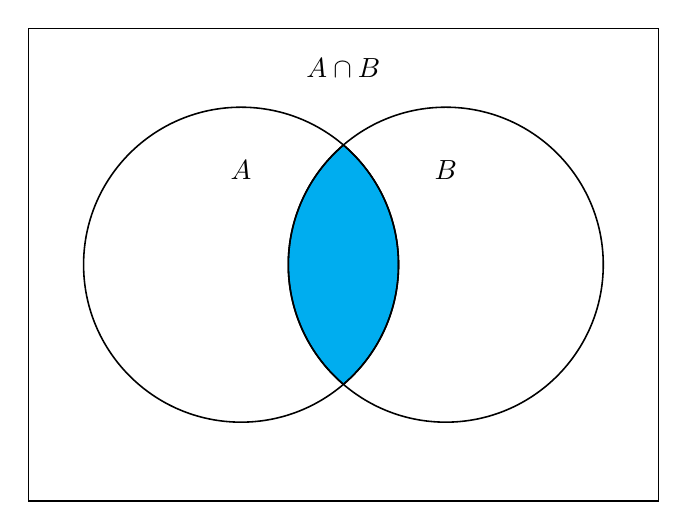
\begin{tikzpicture}[line width=0.2mm]
    % Coordinates for the centers of the circles.
    \coordinate (C1) at (-1.3, 0);
    \coordinate (C2) at ( 1.3, 0);

    % Coordinates for the labels.
    \coordinate (A) at (-1.3, 1.2);
    \coordinate (B) at ( 1.3, 1.2);
    \coordinate (I) at ( 0.0, 2.5);

    % Rectangle indicating the universe set.
    \draw (-4, -3) rectangle (4, 3);

    % Fill in the circle with cyan.
    \draw[fill=cyan] (0, -1.51987) arc(-49.46:49.46:2) arc(130.54:229.46:2);

    % Give outlines to the circles.
    \draw (C1) circle (2);
    \draw (C2) circle (2);

    % Labels.
    \node at (A) {$A$};
    \node at (B) {$B$};
    \node at (I) {$A\cap{B}$};
\end{tikzpicture}
            \caption{Venn Diagrams for Intersections}
            \label{fig:Union_Intersection_venn_diagram}
        \end{figure}
        \begin{ltheorem}{Commutative Law of Intersections}
                        {Commut_Law_Intersec}
            If $A$ and $B$ are sets, then $A\cap{B}=B\cap{A}$.
        \end{ltheorem}
        \begin{proof}
            For if $x\in{A}\cap{B}$, then $x\in{A}$ and
            $x\in{B}$. But then $x\in{B}$ and $x\in{A}$,
            and therefore $x\in{B}\cap{A}$
            (Def.~\ref{def:Intersection_of_Two}). But then
            for all $x\in{A}\cap{B}$ it is true that
            $x\in{B}\cap{A}$, and therefore
            $A\cup{B}\subseteq{B}\cup{A}$
            (Def.~\ref{def:Subsets}). Similarly,
            $B\cap{A}\subseteq{A}\cap{B}$, and thus
            $A\cap{B}=B\cap{A}$ (Def.~\ref{def:Equal_Sets}).
            Therefore, etc.
        \end{proof}
        \begin{theorem}
            \label{thm:Intersection_is_Smaller}%
            If $A$ snd $B$ are sets, then
            $A\cap{B}\subseteq{A}$.
        \end{theorem}
        \begin{proof}
            If $x\in{A}\cap{B}$, then $x\in{A}$ and
            $x\in{B}$, and thus $x\in{A}$. Therefore, etc.
        \end{proof}
        \begin{theorem}
            \label{thm:Intersection_with_Lesser_Set}%
            If $A$, $B$, and $C$ are sets, and if
            $B\subseteq{C}$, then
            $A\cap{B}\subseteq{A}\cap{C}$.
        \end{theorem}
        \begin{proof}
            For if $x\in{A}\cap{B}$, then $x\in{A}$ and
            $x\in{B}$ (Def.~\ref{def:Intersection_of_Two}).
            But $B$ is a subset of $C$, and thus if
            $x\in{B}$, then $x\in{C}$
            (Def.~\ref{def:Subsets}). But then $x\in{A}$ and
            $x\in{C}$, and therefore $x\in{A}\cap{C}$
            (Def.~\ref{def:Intersection_of_Two}). But
            then $A\cap{B}\subseteq{A}\cap{C}$
            (Def.~\ref{def:Subsets}). Therefore, etc.
        \end{proof}
        \begin{theorem}
            \label{thm:Intersection_is_Equal}%
            If $A$ and $B$ are sets, and if
            $A=A\cap{B}$, then $A\subseteq{B}$.
        \end{theorem}
        \begin{proof}
            For suppose not. Then there is an $x\in{A}$ such
            that $x\notin{B}$. But since $A=A\cap{B}$,
            if $x\in{A}$ then $x\in{A}\cap{B}$
            (Def.~\ref{def:Equal_Sets}). But if
            $x\in{A}\cap{B}$, then $x\in{B}$
            (Thm.~\ref{thm:Intersection_is_Smaller}),
            a contradiction. Therefore, etc.
        \end{proof}
        \begin{theorem}
            \label{thm:Intersection_of_Subset}%
            If $A$ and $B$ are sets, and if
            $A\subseteq{B}$, then $A\cap{B}=A$.
        \end{theorem}
        \begin{proof}
            For $A\cap{B}\subseteq{A}$
            (Thm.~\ref{thm:Intersection_is_Smaller}). But
            since $A$ is a subset of $B$, if $x\in{A}$, then
            $x\in{B}$ (Def.~\ref{def:Subsets}). But then
            $x\in{A}\cap{B}$
            (Def.~\ref{def:Intersection_of_Two}). Therefore,
            $A\subseteq{A}\cap{B}$ (Def~\ref{def:Subsets})
            and thus $A=A\cap{B}$ (Def~\ref{def:Equal_Sets}).
            Therefore, etc.
        \end{proof}
        \begin{theorem}
            \label{thm:Conv_Intersection_is_Smaller}%
            If $A$ and $B$ are sets, and if
            $A\subseteq{A}\cap{B}$, then $A=A\cap{B}$.
        \end{theorem}
        \begin{proof}
            For $A\cap{B}\subseteq{A}$
            (Thm.~\ref{thm:Intersection_is_Smaller}). But
            by hypothesis, $A\subseteq{A}\cap{B}$, and thus
            $A=A\cap{B}$ (Def.~\ref{def:Equal_Sets}).
            Therefore, etc.
        \end{proof}
        \begin{theorem}
            If $A$ is a set, then
            $\emptyset\cap{A}=\emptyset$.
        \end{theorem}
        \begin{proof}
            For $\emptyset\subseteq{A}$
            (Thm.~\ref{thm:Emptyset_Is_Subset}), and
            therefore $\emptyset\cap{A}=\emptyset$
            (Thm.~\ref{thm:Intersection_of_Subset}).
        \end{proof}
        \begin{theorem}
            \label{thm:First_Assoc_Law_Intersec}%
            If $A$, $B$, and $C$ are sets, then
            $A\cap(B\cap{C})\subseteq(A\cap{B})\cap{C}$.
        \end{theorem}
        \begin{proof}
            For if $x\in{A}\cap(B\cap{C})$, then $x\in{A}$
            and $x\in{B}\cap{C}$
            (Def.~\ref{def:Intersection_of_Two}). But if
            $x\in{B}\cap{C}$, then $x\in{B}$ and $x\in{C}$
            (Def.~\ref{def:Intersection_of_Two}). But then
            $x\in{A}$ and $x\in{B}$, and therefore
            $x\in{A}\cap{B}$
            (Def.~\ref{def:Intersection_of_Two}). But
            then $x\in{A}\cap{B}$ and $x\in{C}$, and
            therefore $x\in(A\cap{B})\cap{C}$
            (Def.~\ref{def:Intersection_of_Two}). Thus,
            $A\cap(B\cap{C})\subseteq(A\cap{B})\cap{C}$
            (Def.~\ref{def:Subsets}). Therefore, etc.
        \end{proof}
        \begin{ltheorem}{Associative Law of Intersections}
              {Assoc_Law_Intersec}
            If $A$, $B$, and $C$ are sets, then
            $A\cap(B\cap{C})=(A\cap{B})\cap{C}$.
        \end{ltheorem}
        \begin{proof}
            For by the Commutative Law of Intersections
            (Thm.~\ref{thm:Commut_Law_Intersec}),
            we have:
            \begin{equation}
                (A\cap{B})\cap{C}=C\cap(A\cap{B})
                                 =C\cap(B\cap{A})
            \end{equation}
            But $C\cap(B\cap{A})\subseteq(C\cap{B})\cap{A}$
            (Thm.~\ref{thm:First_Assoc_Law_Intersec}).
            Again by commutativity, we obtain:
            \begin{equation}
                (C\cap{B})\cap{A}=A\cap(C\cap{B})
                                 =A\cap(B\cap{C})
            \end{equation}
            Therefore,
            $(A\cap{B})\cap{C}\subseteq{A}\cap(B\cap{C})$.
            But $A\cap(B\cap{C})\subseteq(A\cap{B})\cap{C}$
            (Thm.~\ref{thm:First_Assoc_Law_Intersec}),
            and thus $A\cap(B\cap{C})=(A\cap{B})\cap{C}$
            (Def.~\ref{def:Equal_Sets}). Therefore, etc.
        \end{proof}
        \begin{theorem}
            \label{thm:Redundant_Intersection}%
            If $A$, $B$, and $C$ are sets and if
            $B\subseteq{A}$, then
            $A\cap(B\cap{C})=B\cap{C}$.
        \end{theorem}
        \begin{proof}
            For $A\cup(B\cup{C})\subseteq{B}\cup{C}$
            (Thm.~\ref{thm:Intersection_is_Smaller}). But
            $A\cap(B\cap{C})=(A\cap{B})\cap{C}$
            (Thm.~\ref{thm:Assoc_Law_Intersec}).
            And since $B$ is a subset of $A$,
            $A\cap{B}=A$
            (Thm.~\ref{thm:Intersection_of_Subset}),
            and thus $(A\cap{B})\cap{C}=B\cap{C}$. Thus,
            $B\cap{C}=A\cap(B\cap{C})$
            (Thm.~\ref{thm:Equality_Transitive}).
            Therefore, etc.
        \end{proof}
        \begin{theorem}
            \label{thm:First_Pseudo_Dist_Law_Union}%
            If $A$, $B$, and $C$ are sets, then
            $(B\cap{C})\subseteq(A\cup{B})\cap(A\cup{C})$.
        \end{theorem}
        \begin{proof}
            For $B\subseteq{A}\cup{B}$
            (Thm.~\ref{thm:Union_is_Bigger}). But then
            $B\cap{C}\subseteq(A\cup{B})\cap{C}$
            (Thm.~\ref{thm:Intersection_with_Lesser_Set}).
            But $C\subseteq{A}\cup{C}$
            (Thm.~\ref{thm:Union_is_Bigger}), and thus
            $(A\cup{B})\cap{C}%
             \subseteq(A\cup{B})\cap{A}\cup{C}$
            (Thm.~\ref{thm:Intersection_with_Lesser_Set}).
            But it was just proved that
            $B\cap{C}\subseteq(A\cup{B})\cap{C}$, and
            therefore by transivity,
            $(B\cap{C})\subseteq(A\cup{B})\cap(A\cup{C})$
            (Thm.~\ref{thm:Subset_is_Transitive}).
            Therefore, etc.
        \end{proof}
        \begin{ltheorem}{Distributive Law of Unions}
              {Distributive_Law_Union}
            If $A$, $B$, and $C$ are sets, then
            $A\cup(B\cap{C})=(A\cup{B})\cap(A\cup{C})$.
        \end{ltheorem}
        \begin{proof}
            For $(B\cap{C})\subseteq(A\cup{B})\cap(A\cup{C})$
            (Thm.~\ref{thm:First_Pseudo_Dist_Law_Union}).
            But then:
            \begin{equation}
                A\cup(B\cap{C})\subseteq
                A\cup\Big((A\cup{B})\cap(A\cup{C})\Big)
            \end{equation}
            But $A\cup((A\cup{B})\cap(A\cup{C}))%
                 =(A\cup{B})\cap(A\cup{C})$, and therefore:
            \begin{equation}
                A\cup(B\cap{C})\subseteq
                (A\cup{B})\cap(A\cup{C})
            \end{equation}
        \end{proof}
        \begin{ltheorem}{Distributive Law of Intersections}
              {Distributive_Law_Intersections}
            If $A$, $B$, and $C$ are sets, then
            $A\cap(B\cup{C})=(A\cap{B})\cup(A\cap{C})$.
        \end{ltheorem}
        \begin{proof}
            Hi
        \end{proof}
        If $A$ and $B$ are sets, and if
        $C\subseteq{A}\cup{B}$, then
        either $C\subseteq{A}$ or $C\subseteq{B}$, or both.
        It is possible that $C\subseteq{A}\cup{B}$ and yet
        $C$ and $B$ have no elements in common, as long
        as $C\subseteq{A}$. As an example,
        take $A$ and $B$ to be disjoint sets. Then
        $A\subseteq{A}\cup{B}$, yet $A$ and $B$ have no
        elements in common. If $C\subseteq{A}\cap{B}$, then
        it must be true that $C\subseteq{A}$ and
        $C\subseteq{B}$.
        Using arithmetic as an analogy, the empty set
        acts somewhat like a zero element. It is an identity
        element under set unions, and collapses everything
        down to zero under set intersections. Continuing
        with this analogy, we discuss set difference.
        \begin{ldefinition}{Set Difference}{Set_Difference}
            The set difference of a set $A$ with respect to
            a set $B$, denoted $B\setminus{A}$, is the set:
            \begin{equation}
                B\setminus{A}=\{x\in{B}:x\notin{A}\}
            \end{equation}
        \end{ldefinition}
        \begin{ldefinition}{Symmetric Difference}
              {Symmetric_Difference}
            The symmetric difference of $A$ and $B$, denoted
            $A\ominus{B}$, is the set:
            \begin{equation}
                A\ominus{B}
                =(A\cup{B})\setminus(A\cap{B})
            \end{equation}
        \end{ldefinition}
        While set difference appears similar to subtraction,
        the two have their differences. For any two real
        numbers $a$ and $b$, it is always true that
        $b=a-(a-b)$. For sets this is not true. For let $A$
        be the empty set, and let $B$ be non-empty.
        Then $A\setminus(A\setminus{B})=\emptyset$, which
        is not $B$. Set differences can not be easily
        simplified. The notion is not associative, nor is it
        commutative. If there is a larger \textit{universe}
        set, then set difference can be related to
        intersection.
        \begin{theorem}
            \label{thm:Set_Difference_As_Intersection}%
            If $A$, $B$, and $C$ are sets, and if
            $A\subseteq{C}$ and $B\subseteq{C}$, then:
            \begin{equation}
                B\setminus{A}=B\cap(C\setminus{A})
            \end{equation}
        \end{theorem}
        \begin{proof}
            For if $x\in{B}\setminus{A}$, then
            $x\in{B}$ and $x\notin{A}$. But
            $B\subseteq{C}$, and thus if $x\in{B}$, then
            $x\in{C}$. But if $x\notin{A}$, then
            $x\in{C}\setminus{A}$. Therefore
            $B\setminus{A}\subseteq{B}\cap(C\setminus{A})$.
            Similarly,
            $B\cap(C\setminus{A})\subseteq{B}\setminus{A}$,
            and therefore
            $B\setminus{A}={B}\cap(C\setminus{A})$.
        \end{proof}
        Similar to unions and intersections,
        set differences and symmetric differences can be
        visualized by Venn diagrams, as shown in
        Fig.~\ref{fig:Difference_Sym_Venn_Diagram}.
        \begin{figure}[H]
            \centering
            \caption{Caption}
            \label{fig:Difference_Sym_Venn_Diagram}
        \end{figure}
        The concept of set difference can then be used to
        define the concept of complement.
        \begin{ldefinition}{Complement}{Complement}
            The complement of a set $A$ with respect to a set
            $\Omega$, denoted $A^{C}$, is the set:
            \begin{equation}
                A^{C}=\Omega\setminus{A}
            \end{equation}
        \end{ldefinition}
        Thm.~\ref{thm:Set_Difference_As_Intersection}
        can then be translated into the notation of
        complements as follows:
        \begin{theorem}
            If $A$, $B$, and $\Omega$ are sets,
            $A,B\subseteq\Omega$, and if $A^{C}$ is the
            complement of $A$ with respect to $\Omega$, then:
            \begin{equation}
                B\setminus{A}=B\cap{A}^{C}
            \end{equation}
        \end{theorem}
        \begin{proof}
            By the definition of complement,
            $A^{C}=\Omega\setminus{A}$.
            As $A\subseteq\Omega$ and $B\subseteq\Omega$, by
            Thm.~\ref{thm:Set_Difference_As_Intersection},
            $B\setminus{A}=B\cap(\Omega\setminus{A})$,
            and therefore $B\setminus{A}=B\cap{A}^{C}$.
        \end{proof}
        The main result about complements are known as
        DeMorgan's Laws. The laws relate unions and
        intersections by means of complements. The general
        laws hold for arbitrary unions and arbitrary
        intersections, as will be shown later.
        \begin{ftheorem}{DeMorgan's Laws}{MEASURE_DEMORGAN}
            If $A$, $B$, and $\Omega$ are sets, if
            $A\subseteq\Omega$ and $B\subseteq\Omega$, then:
            \begin{subequations}
                \begin{align}
                    \big(A\cap{B}\big)^{C}
                        &=A^{C}\cup{B}^{C}\\
                    \big(A\cup{B}\big)^{C}
                        &=A^{C}\cap{B}^{C}
                \end{align}
            \end{subequations}
        \end{ftheorem}
        \begin{proof}
            It do.
        \end{proof}
        With this, we can prove some results about
        set differences.
        \begin{theorem}
            If $A$ and $B$ are sets, then:
            \begin{equation}
                A=\big(A\cap{B}\big)
                    \cup\big(A\setminus{B}\big)
            \end{equation}
        \end{theorem}
        \begin{proof}
            For let $\Omega=A\cup{B}$. Then
            $A\subseteq\Omega$ and $B\subseteq\Omega$,
            and thus:
            \begin{subequations}
                \begin{align}
                    \big(A\cap{B})\cup\big(A\setminus{B}\big)
                    &=\big(A\cap{B}\big)
                        \cup\big(A\cap{B}^{C}\big)\\
                    &=A\cap(B\cup{B}^{C})\\
                    &=A\cap\Omega
                \end{align}
            \end{subequations}
            But by Thm.~\ref{thm:Intersection_is_Smaller},
            $A\cap\Omega=A$. Therefore, etc.
        \end{proof}
        \begin{theorem}
            If $A$, $B$, and $C$ are sets, then:
            \begin{equation}
                A\cap\big(B\setminus{C}\big)
                =\big(A\cap{B}\big)\cap\big(A\setminus{C}\big)
            \end{equation}
        \end{theorem}
        \begin{proof}
            For:
            \begin{subequations}
                \begin{align}
                    A\cap\big(B\setminus{C}\big)
                    &=A\cap\big(B\cap{C}^{C}\big)\\
                    &=\big(A\cap{A}\big)
                        \cap\big(B\cap{C}^{C}\big)\\
                    &=\big(A\cap{B}\big)
                        \cap\big(A\cap{C}^{C}\big)\\
                    &=\big(A\cap{B}\big)
                        \cap\big(A\setminus{C}\big)
                \end{align}
            \end{subequations}
        \end{proof}
        Intersections do distribute over set differences.
        \begin{theorem}
            If $A$, $B$, and $C$ are sets, then:
            \begin{equation}
                A\cap(B\setminus{C})=
                (A\cap{B})\setminus(A\cap{C})
            \end{equation}
        \end{theorem}
        \begin{proof}
            For:
            \begin{subequations}
                \begin{align}
                    \big(A\cap{B}\big)\setminus
                        \big(A\cap{C}\big)
                    &=\big(A\cap{B}\big)
                        \cap\big(A\cap{C}\big)^{C}\\
                    &=\big(A\cap{B}\big)
                        \cap\big(A^{C}\cup{C}^{C}\big)\\
                    &=\big[\big(A\cap{B}\big)\cap{A}^{C}\big]
                        \cup\big[\big({A}\cap{B}\big)
                        \cap{C}^{C}\big]\\
                    &=\big[\big(A\cap{A}^{C}\big)\cap{B}\big]
                        \cup\big[\big(A\cap{B}\big)
                        \cap{C}^{C}\big]\\
                    &=\emptyset\cup\big[\big(A\cap{B}\big)
                        \cap{C}^{C}\big]\\
                    &=\big(A\cap{B}\big)\cap{C}^{C}\\
                    &=A\cap\big(B\cap{C}^{C}\big)\\
                    &=A\cap\big(B\setminus{C}\big)
                \end{align}
            \end{subequations}
            Therefore, etc.
        \end{proof}
        Unions do not, however. For let $A$ be non-empty
        and let $A=B=C$. Then $A\cup(B\setminus{C})=A$, but
        $(A\cup{B})\setminus(A\cup{C})=\emptyset$.
        DeMorgan's Laws hold for arbitrary collections
        of set. If $I$ is some indexing set:
        \begin{align}
            \Big(\bigcup_{\alpha\in{I}}A_{\alpha}\Big)^{C}
            &=\bigcap_{\alpha\in{I}}A_{\alpha}^{C}\\
            \Big(\bigcap_{\alpha\in{I}}A_{\alpha}\Big)^{C}
            &=\bigcup_{\alpha\in{I}}A_{\alpha}^{C}
        \end{align}
        The set operations thus define binary operations
        on the power set of a set $\Omega$. It's important
        to note the notation. An element of $\Omega$ may
        be anything, while an element of
        $\mathcal{P}(\Omega)$ is a subset of $\Omega$.
        That is, the \textit{points} of $\mathcal{P}(\Omega)$
        are themselves sets. Thus, union, intersection,
        etc., define binary operations on
        $\mathcal{P}(\Omega)$. Given two subsets of
        $\Omega$, $A$ and $B$, $A\cup{B}$ is another
        subset of $\Omega$, as is $A\cap{B}$, and so on.
        The complement can also be seen as a unary operator
        on $\mathcal{P}(\Omega)$.
        \section{Cardinality}
    As mentioned before, there is a way to discuss the size of sets in a manner
    that allows one to be precise when stating \textit{the set A is larger than}
    \textit{the set B}. If two sets are small enough, we can simply count out
    the number of elements contained in each and compare sets this way. For an
    infinite set it doesn't make sense to talk about the \textit{number} of
    elements, but we can still specify what it means two sets to have the same
    size. Sets $A$ and $B$ are equivalent if there exists a bijection
    $f:A\rightarrow{B}$. We then say that $A$ and $B$ have the same cardinality,
    and we denote this by $\textrm{Card}(A)=\textrm{Card}(B)$. A finite set is a
    set $A$ such that there is a bijection between $A$ and $\mathbb{Z}_{n}$, for
    some $n\in\mathbb{N}$. We can then view the elements of $A$ as
    $A=\{a_{1},\hdots,a_{n}\}$. A countable set is a set $A$ such that there is
    a bijection between $A$ and $\mathbb{N}$. These notions were first developed
    by Georg Cantor\index{Cantor, Georg}, and one natural question would be to
    ask if $\textrm{Card}(\mathbb{N})=\textrm{Card}(\mathbb{N})$? What about
    $\textrm{Card}(\mathbb{N})$ and $\textrm{Card}(\mathbb{R})$? This chapter
    aims to answer these questions, and develop the cardinal numbers along the
    way.
    \subsection{Equivalent Sets}
        \begin{fdefinition}{Equivalent Sets}{Equivalent_Sets}
            Equivalent sets are \glspl{set} $A$ and $B$ such that there exists a
            \gls{bijective function} $f:A\rightarrow{B}$.
        \end{fdefinition}
        The notion of equivalent sets defines an equivalence relation on sets.
        That is, the notion is reflexive, symmetric, and transitive.
        \begin{theorem}
            If $A$ is a set, then $A$ is equivalent to $A$.
        \end{theorem}
        \begin{proof}
            For the identity mapping $\textrm{id}_{A}:A\rightarrow{A}$ is a
            bijective function.
        \end{proof}
        \begin{theorem}
            If $A$ and $B$ are sets and if $A$ is equivalent to $B$, then $B$ is
            equivalent to $A$.
        \end{theorem}
        \begin{proof}
            For if $A$ is equivalent to $B$, then there is a bijection
            $f:A\rightarrow{B}$. But if $f$ is a bijection, then the inverse
            function $f^{-1}:B\rightarrow{A}$ is well-defined and is a
            bijection. Thus $B$ is equivalent to $A$.
        \end{proof}
        \begin{theorem}
            If $A$, $B$, and $C$ are sets, if $A$ is equivalent to $B$, and if
            $B$ is equivalent to $C$, then $A$ is equivalent to $C$.
        \end{theorem}
        \begin{proof}
            For if $A$ is equivalent to $B$, then there is a bijection
            $f:A\rightarrow{B}$. But if $B$ is equivalent ot $C$, then there is a
            bijection $g:B\rightarrow{C}$. But then $g\circ{f}:A\rightarrow{C}$ is a
            bijection, and thus $A$ and $C$ are equivalent.
        \end{proof}
        A bijection is a function that is both injective and surjective. Thus, two
        equivalent sets can be put into a one-to-one correspondence and can be said
        to have the same size. We then say that $A$ and $B$ have the same
        cardinality. The notation is written as $|A|=|B|$ or $\Card(A)=\Card(B)$.
        Cardinality splits sets into one of three categories.
        \begin{ldefinition}{Finite Sets}{Finite_Sets}
            A finite set is a set $A$ such that there exists
            an $n\in\mathbb{N}$ such that there is a
            bijection $f:\mathbb{Z}_{n}\rightarrow{A}$, or
            such that $A=\emptyset$.
        \end{ldefinition}
        Sets that are not finite are called infinite. There
        are two types of infinite sets. Let $\mathbb{N}$
        denote the set of positive integers, or
        \textit{natural} numbers.
        \begin{ldefinition}{Countably Infinite Sets}
              {Countably_Infinite}
            A countably infinite set is a set $A$ such that
            is a bijection $f:\mathbb{N}\rightarrow{A}$.
        \end{ldefinition}
        Combining the notions of finite sets and countably
        infinite sets, we get the notion of
        \textit{countable} sets.
        \begin{ldefinition}{Countable Sets}
              {Countable_Sets}
            A countable set is a set $A$ such that $A$ is
            either finite or countably infinite.
        \end{ldefinition}
        Countable sets are also called \textit{listable}.
        This is because if $A$ is a countably infinite set,
        and if $a:\mathbb{N}\rightarrow{A}$ is a bijection,
        we can write $A$ as:
        \begin{equation}
            A=\{\;a_{n}\,:\,n\in\mathbb{N}\;\}
            =\{\,a_{1},\,a_{2},\,\dots,\,a_{k},\,\dots\,\}
        \end{equation}
        If $A$ is finite, and if
        $a:\mathbb{Z}_{n}\rightarrow{A}$ is a
        bijection, then we can write:
        \begin{equation}
            A=\{\;a_{n}\,:\,n\in\mathbb{Z}_{n}\;\}
             =\{\,a_{1},\,\dots,\,a_{n}\,\}
        \end{equation}
        Recall that functions $a:\mathbb{N}\rightarrow{A}$
        are called \textit{sequences}, and the image of
        $n\in\mathbb{N}$ is written $a_{n}$, rather than
        $a(n)$.
        \begin{example}
            The set of all positive even integers is
            countable. For let $\mathbb{N}_{e}$ be the
            set of all even integers and define
            $f:\mathbb{N}\rightarrow\mathbb{N}_{e}$ be
            $f(n)=2n$ for all $n\in\mathbb{N}$. This is
            a bijection, and thus $\mathbb{N}_{e}$ is
            countable. The set of all odd positive integers
            is countable, as shown by letting
            $f(n)=2n-1$. Even though the set of even
            integers may seem ``smaller,'' than the set of
            all integers, they are equivalent. The set of
            all integers $\mathbb{Z}$ is also countable.
            For let $f:\mathbb{N}\rightarrow\mathbb{Z}$
            be defined as:
            \begin{equation}
                f(n)=
                \begin{cases}
                    \frac{1}{2}(n-1),&n\textrm{ odd}\\
                    -\frac{n}{2},&n\textrm{ even}
                \end{cases}
            \end{equation}
        \end{example}
        Any set that is infinite (Not finite) contains a
        countable subset. Thus, $\mathbb{N}$ can be
        considered as the \textit{smallest} infinite set.
        \begin{theorem}
            If $A$ is an infinite set, then there exists
            $S\subseteq{A}$ such that $S$ is countable.
        \end{theorem}
        \begin{proof}
            For as $A$ is infinite, for all $n\in\mathbb{N}$
            there exists a set $B\subseteq{A}$ such that
            $|B|=n$. For all $n\in\mathbb{N}$,
            define the following:
            \begin{equation}
                \mathcal{S}_{n}=\{B\subseteq{A}:|B|=n\}
            \end{equation}
            Let $\mathcal{S}$ be defined as:
            \begin{equation}
                \mathcal{S}=\{\mathcal{S}_{n}:n\in\mathbb{N}\}
            \end{equation}
            Then $\mathcal{S}$ is countable, for
            $a:\mathbb{N}\rightarrow\mathcal{S}$ defined
            by $a_{n}=\mathcal{S}_{n}$ is a bijection.
            By the axiom of choice, there is a function:
            \begin{equation}
                \alpha:\mathcal{S}\rightarrow
                \bigcup_{n=1}^{\infty}\mathcal{S}_{n}
            \end{equation}
            Such that, for all $x\in\mathcal{S}$,
            $\alpha(x)\in{x}$. But then, for all
            $x\in\mathcal{S}$, $\alpha(x)$ is a subset
            of $A$. But for all $x\in\mathcal{S}$, there
            is an $n\in\mathbb{N}$ such that
            $a_{n}=x$. Thus, let $S$ be the following:
            \begin{equation}
                S=\bigcup_{n=1}^{\infty}\alpha(a_{n})
            \end{equation}
        \end{proof}
        In the absence of the requirement that $a\cap{b}=\emptyset$ for all
        pairs in $\mathcal{U}$, we still have that the union is, at most,
        countable. The mapping we found would be a \textit{surjection}, rather
        than a bijection. The union is then either finite or countable. The
        Cantor-Schr\"{o}der-Bernstein Theorem can often be used to help identify
        the size of a set. This says that if $A$ and $B$ are sets such that
        there exists a surjective function $f:A\rightarrow{B}$ and a surjective
        function $g:B\rightarrow{A}$, then there is a bijective function
        $h:A\rightarrow{B}$. The requirement that $f$ and $g$ both be surjective
        can be replaced with the requirement that they both be injective. This
        is similar to saying that if $\Card(A)\leq\Card(B)$ and
        $\Card(B)\leq\Card(A)$, then $\Card(A)=\Card(B)$. Here, $\Card(A)$
        denotes the \textit{cardinality} of the set $A$.
        \begin{lexample}{Countable Sets}{Countable_Sets}
            There are many commonly discussed sets that are
            countably infinite. $\mathbb{N}$ is a trivial
            such example, but also $\mathbb{N}_{e}$ and
            $\mathbb{N}_{o}$, the sets of even and odd
            positive integers, respectively. For consider as
            bijections the following functions:
            \par
            \begin{subequations}
                \begin{minipage}[b]{0.49\textwidth}
                    \centering
                    \begin{equation}
                        f_{e}(n)=2n
                    \end{equation}
                \end{minipage}
                \hfill
                \begin{minipage}[b]{0.49\textwidth}
                    \centering
                    \begin{equation}
                        f_{0}(n)=2n-1
                    \end{equation}
                \end{minipage}
                \par\vspace{2.5ex}
                The set of all integers, $\mathbb{Z}$ is also
                countable, as shown in
                Fig.~\ref{fig:Bijection_N_and_Z}.
                One bijection is:
                \begin{equation}
                    f(n)=
                    \begin{cases}
                        \frac{n}{2},&n\mod{2}=0\\
                        \frac{1-n}{2},&n\mod{2}=1
                    \end{cases}
                \end{equation}
            \end{subequations}
            Any subset of $\mathbb{Z}$ is countable,
            and this is true of any countable set.
        \end{lexample}
        \begin{figure}[H]
            \centering
            \captionsetup{type=figure}
            \documentclass[crop,class=article]{standalone}
%----------------------------Preamble-------------------------------%
\usepackage{tikz}
\usepackage{amssymb}
\usetikzlibrary{arrows.meta}
%--------------------------Main Document----------------------------%
\begin{document}
    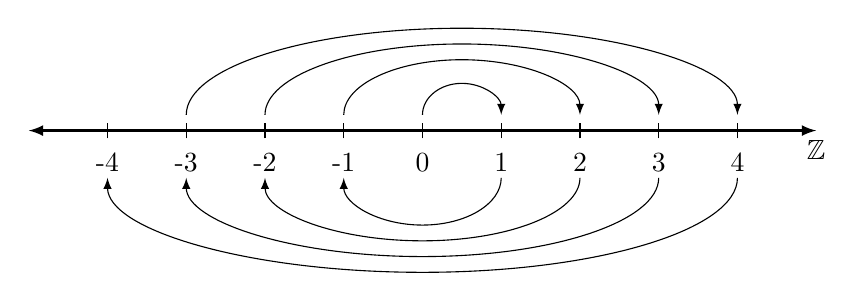
\begin{tikzpicture}[%
        >=latex
    ]
        \draw[<->, thick] (-5, 0) to (5, 0) node[below] {$\mathbb{Z}$};
        \foreach\x in {-4, -3, -2, -1, 0, 1, 2, 3, 4}{%
            \draw (\x, -0.1) to (\x, 0.1);
            \node at (\x, -0.4) {\x};
        }
        \draw[->] (0, 0.2) arc(180:0:0.5 and 0.4);
        \draw[->] (1, -0.6) arc(0:-180:1 and 0.6);
        \draw[->] (-1, 0.2) arc(180:0:1.5 and 0.7);
        \draw[->] (2, -0.6) arc(0:-180:2 and 0.8);
        \draw[->] (-2, 0.2) arc(180:0:2.5 and 0.9);
        \draw[->] (3, -0.6) arc(0:-180:3 and 1);
        \draw[->] (-3, 0.2) arc(180:0:3.5 and 1.1);
        \draw[->] (4, -0.6) arc(0:-180:4 and 1.2);
    \end{tikzpicture}
\end{document}
            \caption{Diagram of a Bijection Between
                     $\mathbb{N}$ and $\mathbb{Z}$.}
            \label{fig:Bijection_N_and_Z}
        \end{figure}
        One of the standard results about countable sets is
        that their subsets are also countable. This theorem
        relies, in a very subtle way, the use of the axiom
        of choice. There are a few stepping stones to get
        there. We will accept the various
        Cantor-Schr\"{o}eder-Bernstein theorems, which say
        the following:
        \begin{ltheorem}
              {First Cantor-Schr\"{o}eder-Bernstein Theorem}
              {First_Cantor_Schroeder_Bernstein}
            If $A$ and $B$ are sets such that there is an injective
            function $f:A\rightarrow{B}$ and an injective function
            $g:B\rightarrow{A}$, then there is a bijective function
            $h:A\rightarrow{B}$.
        \end{ltheorem}
        \begin{ltheorem}
              {Second Cantor-Schr\"{o}eder-Bernstein Theorem}
              {Second_Cantor_Schroeder_Bernstein}
            If $A$ and $B$ are sets such that there is a surjective
            function $f:A\rightarrow{B}$ and a surjective function
            $g:B\rightarrow{A}$, then there is a bijective function
            $h:A\rightarrow{B}$.
        \end{ltheorem}
        \par\hfill\par
        Using cardinalities, this says that if
        $\Card(A)\leq\Card(B)$ and $\Card(B)\leq\Card(A)$, then
        $\Card(A)=\Card(B)$. With this notation it becomes more
        intuitive. We will use this to prove that various sets are
        countable. Many sets that appear to be larger than $\mathbb{N}$
        can shown to to be the same size as $\mathbb{N}$ by finding
        a simple injective function, without finding an explicit
        bijection.
        \begin{ltheorem}
              {Third Cantor-Schr\"{o}eder-Bernstein Theorem}
              {Third_Cantor_Schroeder_Bernstein}
            If $A$, $B$, and $C$ are sets such that
            $A\subseteq{B}\subseteq{C}$, and if $A$ and $C$ are equivalent
            sets, then $B$ and $C$ are equivalent sets.
        \end{ltheorem}
        \par\hfill\par
        This says that if $\Card(A)\leq\Card(B)\leq\Card(C)$,
        and if $\Card(A)=\Card(C)$, then $\Card(B)=\Card(C)$.
        \begin{theorem}
            \label{thm:Measure_Theory_NxN_Is_Countable}
            $\mathbb{N}\times\mathbb{N}$ is countably infinite.
        \end{theorem}
        \begin{proof}
            There is a trivial injection
            $f:\mathbb{N}\rightarrow\mathbb{N}\times\mathbb{N}$
            defined by:
            \begin{equation}
                f(n)=(n,0)
            \end{equation}
            There is also an injection
            $g:\mathbb{N}\times\mathbb{N}\rightarrow\mathbb{N}$
            defined by:
            \begin{equation}
                g(n.m)=2^{n}3^{m}
            \end{equation}
            Since 2 and 3 are co-prime, if
            $g(n_{1},m_{1})=g(n_{2},m_{2})$, then
            $(n_{1},m_{1})=(n_{2},m_{2})$. Thus, $g$ is an injection.
            By the Cantor-Schr\"{o}eder-Bernstein Theorem, there is a
            bijection $h:\mathbb{N}\rightarrow\mathbb{N}\times\mathbb{N}$.
        \end{proof}
        One can intuitively see that the set of all positive
        rational numbers $\mathbb{Q}^{+}$ is countable by examining
        the zig-zag pattern shown in
        Fig.~\ref{fig:Bijection_N_and_Q_Plus}.
        Thm.~\ref{thm:Measure_Theory_NxN_Is_Countable} also
        shows this in a more rigorous way that. We can create
        a one-to-one correspondence with
        $\mathbb{N}\times\mathbb{N}$ by mapping
        $pq^{\minus{1}}\mapsto(p,q)$. Thus $\mathbb{Q}^{+}$
        and $\mathbb{N}\times\mathbb{N}$ are equivalent sets.
        But $\mathbb{N}\times\mathbb{N}$ and $\mathbb{N}$
        are equivalent sets, and therefore $\mathbb{Q}^{+}$
        is countable.
        Thm.~\ref{thm:Measure_Theory_NxN_Is_Countable} can also be used
        to show that the countable union of countable sets is also
        countable.
        \begin{ltheorem}{Equivalence of Countable Sets}
              {Countable_iff_exists_inj_to_N}
            A set $A$ is countable if and only if there is an injective
            function $f:A\rightarrow\mathbb{N}$.
        \end{ltheorem}
        Thm.~\ref{thm:Countable_iff_exists_inj_to_N} seems
        intuitively obvious, the injective function is
        simply the listing function. For a finite set, this
        is precisely how one constructs such an injection.
        For an infinite set $A$, this is equivalent to
        showing that any infinite subset of $\mathbb{N}$ is
        equivalent to $\mathbb{N}$. The standard proof
        using \textit{induction}, but actually has the axiom
        of choice underlying it.
        \begin{theorem}
            If $\mathcal{A}$ is a countably infinite set
            such that, for all $A\in\mathcal{A}$, $A$ is
            a non-empty countable set, then the set:
            \begin{equation}
                S=\bigcup_{A\in\mathcal{A}}A
            \end{equation}
            Is a countable set.
        \end{theorem}
        \begin{proof}
            If $\mathcal{F}$ is finite, then we are done. Suppose not.
            Let $A:\mathbb{N}\rightarrow\mathcal{A}$ be a bijection,
            and define:
            \begin{equation}
                S=\bigcup_{n\in\mathbb{N}}A_{n}
            \end{equation}
            Also, let:
            \begin{equation}
                \mathcal{F}_{n}
                =\{f:A_{n}\rightarrow\mathbb{N}:
                    f\textrm{ is injective}\}
            \end{equation}
            Since, for all $n\in\mathbb{N}$, $A_{n}$ is
            non-empty and countable, $\mathcal{F}_{n}$
            is non-empty. Let:
            \begin{equation}
                \mathcal{F}
                =\bigcup_{n\in\mathbb{N}}\mathcal{F}_{n}
            \end{equation}
            Thus, by the axiom of choice, there is a function
            $F:\mathbb{N}\rightarrow\mathcal{F}$ such that, for all
            $n\in\mathbb{N}$, $F_{n}\in\mathcal{F}_{n}$. For
            $x\in{S}$, let:
            \begin{equation}
                \varphi_{x}
                =\inf\{n\in\mathbb{N}:x\in{A}_{n}\}
            \end{equation}
            By the well-ordering of $\mathbb{N}$, for all
            $x\in{S}$, $\varphi_{x}$ is well defined. Let
            $\phi:S\rightarrow\mathbb{N}\times\mathbb{N}$
            be defined by:
            \begin{equation}
                \phi(x)
                =\big(\varphi_{x},F_{\varphi_{x}}(x)\big)
            \end{equation}
            Then $\phi$ is an injection. For if
            $\big(\varphi_{x},F_{\varphi_{x}}(x)\big)=%
             \big(\varphi_{y},F_{\varphi_{x}}(y)\big)$, then
            $\varphi_{x}=\varphi_{y}$, and thus
            $F_{\varphi(x)}(x)=F_{\varphi(x)}(y)$. But
            $F_{\varphi_{x}}$ is an injection, and
            thus $x=y$. Therefore $\phi$ is an injection.
            But $\mathbb{N}\times\mathbb{N}$ and $\mathbb{N}$
            are equivalent sets, and thus there's an
            injection $f:\mathbb{N}\times\mathbb{N}$. And
            the composition of injective functions is again
            injective, and thus
            $\phi\circ{f}:S\rightarrow\mathbb{N}$ is an
            injective function. But by
            Thm.~\ref{thm:Countable_iff_exists_inj_to_N},
            if there is an injective function
            $f:S\rightarrow\mathbb{N}$, then $S$ is
            countable. Therefore, etc.
        \end{proof}
        \begin{theorem}
            If $X$ is infinite, then there exists a
            countably infinite set $A\subseteq{X}$.
        \end{theorem}
        \begin{proof}
            If $A$ is finite, then we are done. Suppose not.
            For $n\in\mathbb{N}$, let:
            \begin{equation}
                A_{n}
                =\{g:\mathbb{Z}_{n}\rightarrow{A}:f\textrm{ is inective}\}
            \end{equation}
            Also, define:
            \begin{equation}
                \mathcal{F}=\bigcup_{n\in\mathbb{N}}A_{n}
            \end{equation}
            But by the axiom of choice, there is a function
            $f:\mathbb{N}\rightarrow\mathcal{F}$ such that
            $f_{n}\in{A}_{n}$. But then, for all
            $n\in\mathbb{N}$, the range of $f_{n}$ is finite.
            \begin{equation}
                A=\bigcup_{n\in\mathbb{N}}f_{n}
                    \Big(\mathbb{Z}_{n}\Big)
            \end{equation}
            Then $A\subseteq{X}$ is countably infinite.
        \end{proof}
        The set of rational numbers, $\mathbb{Q}$, is also
        countable. We may intuitively think of $\mathbb{N}$
        as being smaller than $\mathbb{Q}$, since there are
        simple \textit{surjections} that can be constructed
        from $\mathbb{Q}$ to $\mathbb{N}$. There is also a
        surjection from $\mathbb{N}$ onto $\mathbb{Q}^{+}$,
        as is shown in Fig.~\ref{fig:Bijection_N_and_Q_Plus}.
        To construct such a surjection, write out all of the
        positive rational numbers in a grid so that $a_{nm}$
        is the number $n/m$. Then zig-zag along the diagonals
        to construct the function. Thus there is a surjection
        $f:\mathbb{Q}^{+}\rightarrow\mathbb{N}$ and a surjection
        $g:\mathbb{N}\rightarrow\mathbb{Q}^{+}$. The
        Cantor-Schr\"{o}eder-Bernstein theorem says that if there is
        surjection from $A$ to $B$ and a surjection from $B$ to $A$, then
        there is a bijection between $A$ and $B$. Therefore there is a
        bijection between $\mathbb{N}$ and $\mathbb{Q}^{+}$, and
        $\mathbb{Q}^{+}$ is countable.
        \begin{figure}[H]
            \centering
            \captionsetup{type=figure}
            \resizebox{0.7\textwidth}{!}{%
                \documentclass[crop,class=article]{standalone}
%----------------------------Preamble-------------------------------%
\usepackage{tikz}
\usetikzlibrary{arrows.meta}
%--------------------------Main Document----------------------------%
\begin{document}
    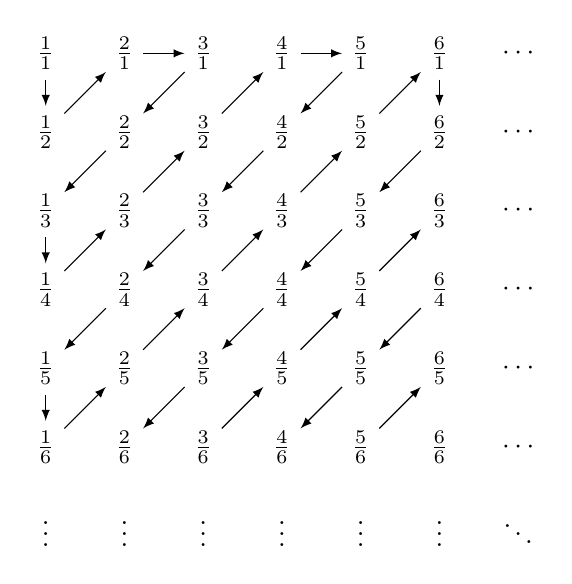
\begin{tikzpicture}[%
        >=latex
    ]
        \foreach\y in {1, 2, 3, 4, 5, 6}{%
            \foreach\x in {1, 2, 3, 4, 5, 6}{%
                \node (\x\y) at (\x, 7-\y) {$\frac{\x}{\y}$};
            }
        }
        \foreach\x in {1, 2, 3, 4, 5, 6}{%
            \node at (7, \x) {$\cdots$};
            \node at (\x, 0) {$\vdots$};
        }
        \node at (7, 0) {$\ddots$};
        \draw[->] (11) to (12);
        \draw[->] (12) to (21);
        \draw[->] (21) to (31);
        \draw[->] (31) to (22);
        \draw[->] (22) to (13);
        \draw[->] (13) to (14);
        \draw[->] (14) to (23);
        \draw[->] (23) to (32);
        \draw[->] (32) to (41);
        \draw[->] (41) to (51);
        \draw[->] (51) to (42);
        \draw[->] (42) to (33);
        \draw[->] (33) to (24);
        \draw[->] (24) to (15);
        \draw[->] (15) to (16);
        \draw[->] (16) to (25);
        \draw[->] (25) to (34);
        \draw[->] (34) to (43);
        \draw[->] (43) to (52);
        \draw[->] (52) to (61);
        \draw[->] (61) to (62);
        \draw[->] (62) to (53);
        \draw[->] (53) to (44);
        \draw[->] (44) to (35);
        \draw[->] (35) to (26);
        \draw[->] (36) to (45);
        \draw[->] (45) to (54);
        \draw[->] (54) to (63);
        \draw[->] (64) to (55);
        \draw[->] (55) to (46);
        \draw[->] (56) to (65);
    \end{tikzpicture}
\end{document}
            }
            \caption{Diagram of a Surjection from
                     $\mathbb{N}$ onto $\mathbb{Q}^{+}$.}
            \label{fig:Bijection_N_and_Q_Plus}
        \end{figure}
        We can modify Fig.~\ref{fig:Bijection_N_and_Q_Plus}
        slightly to create a surjection between $\mathbb{N}$
        and $\mathbb{Q}$, see
        Fig.~\ref{fig:Bijection_N_and_Q}.
        It is important to note that this bijection will not
        preserve the order of the rational numbers. The
        bijection will have to jump around back and forth.
        Any such bijection will be forced to do this, as the
        rationals are everywhere dense on $\mathbb{R}$. Any
        monotonic sequence of $\mathbb{Q}$ cannot possibly
        be a bijection.
        \begin{theorem}
            If $A$ is a countably infinite set and
            $B\subseteq{A}$, then $B$ is countable.
        \end{theorem}
        \begin{proof}
            As $A$ is countably infinite, there is a bijection
            $a:\mathbb{N}\rightarrow{A}$. Define:
            \begin{equation}
                K=\{n\in\mathbb{N}:a_{n}\in{B}\}
            \end{equation}
            As $B\subseteq{A}$,
            this set contains a subsequence of points in
            $\mathbb{N}$ that get mapped into $B$. If $K$ is finite,
            then $B$ is finite, and if not then $K$ is countably
            infinite, and thus $B$ is countably infinite.
        \end{proof}
        \begin{figure}[H]
            \centering
            \captionsetup{type=figure}
            \resizebox{\textwidth}{!}{%
                \documentclass[crop,class=article]{standalone}
%----------------------------Preamble-------------------------------%
\usepackage{tikz}
\usepackage{amsmath}
\usetikzlibrary{arrows.meta}
%--------------------------Main Document----------------------------%
\begin{document}
    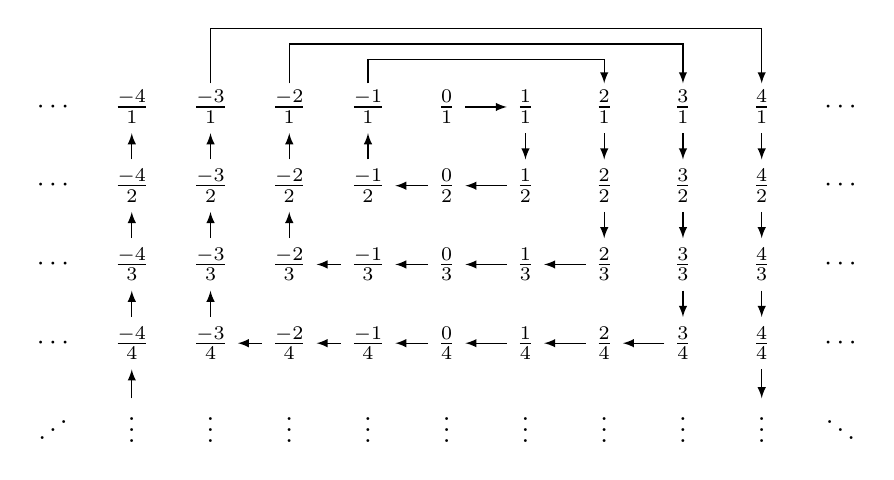
\begin{tikzpicture}[%
        >=latex
    ]
        \foreach\y in {1, 2, 3, 4}{%
            \foreach\x in {-4, -3, -2, -1, 0, 1, 2, 3, 4}{%
                \node (\x\y) at (\x, 7-\y) {$\frac{\x}{\y}$};
            }
        }
        \foreach\x in {-4, -3, -2, -1, 0, 1, 2, 3, 4}{%
            \node at (\x, 2) {$\vdots$};
        }
        \foreach\y in {3, 4, 5, 6}{%
            \node at (5, \y) {$\cdots$};
            \node at (-5, \y) {$\cdots$};
        }
        \node at (5, 2) {$\ddots$};
        \node at (-5, 2) {$\reflectbox{\ensuremath{\ddots}}$};
        \draw[->] (01) to (11);
        \draw[->] (11) to (12);
        \draw[->] (12) to (02);
        \draw[->] (02) to (-12);
        \draw[->] (-12) to (-11);
        \draw[->] (-1, 6.3) to (-1, 6.6)
                            to (2, 6.6)
                            to (2, 6.3);
        \draw[->] (21) to (22);
        \draw[->] (22) to (23);
        \draw[->] (23) to (13);
        \draw[->] (13) to (03);
        \draw[->] (03) to (-13);
        \draw[->] (-13) to (-23);
        \draw[->] (-23) to (-22);
        \draw[->] (-22) to (-21);
        \draw[->] (-2, 6.3) to (-2, 6.8)
                            to (3, 6.8)
                            to (3, 6.3);
        \draw[->] (31) to (32);
        \draw[->] (32) to (33);
        \draw[->] (33) to (34);
        \draw[->] (34) to (24);
        \draw[->] (24) to (14);
        \draw[->] (14) to (04);
        \draw[->] (04) to (-14);
        \draw[->] (-14) to (-24);
        \draw[->] (-24) to (-34);
        \draw[->] (-34) to (-33);
        \draw[->] (-33) to (-32);
        \draw[->] (-32) to (-31);
        \draw[->] (-3, 6.3) to (-3, 7)
                            to (4, 7)
                            to (4, 6.3);
        \draw[->] (41) to (42);
        \draw[->] (42) to (43);
        \draw[->] (43) to (44);
        \draw[->] (44) to (4, 2.3);
        \draw[->] (-4, 2.3) to (-44);
        \draw[->] (-44) to (-43);
        \draw[->] (-43) to (-42);
        \draw[->] (-42) to (-41);
    \end{tikzpicture}
\end{document}
            }
            \caption{Diagram of a Surjection from
                     $\mathbb{N}$ onto $\mathbb{Q}$.}
            \label{fig:Bijection_N_and_Q}
        \end{figure}
        \begin{theorem}
            If $A$ is an infinite set, then there exists a
            countable subset $B\subseteq{A}$.
        \end{theorem}
        \begin{proof}
            If $A$ is infinite then there is an
            $a_{1}\in{A}$. But, as $A$ is infinite,
            $A\setminus\{a_{1}\}$ is infinite, and there
            is an $a_{2}\in{A}\setminus\{a_{1}\}$. Continuing
            we obtain a sequence of distinct elements in $A$.
            Let $B=\{a_{n}:n\in\mathbb{N}\}$. Then
            $B\subseteq{A}$, and $B$ is countable.
        \end{proof}
        \begin{lexample}
            Suppose we have a collection of disjoint intervals
            of $\mathbb{R}$. This collection is either finite
            or countable. For in every interval, choose a
            rational number $q_{n}$. Let
            $A=\{q_{1},q_{2},\hdots\}$. Then
            $A\subseteq\mathbb{Q}$, and thus $A$ is either
            finite or countable. But this is also an enumeration
            of the intervals in the collection, and thus the
            collection is either finite or countable.
        \end{lexample}
        Given a countable collection of sets
        $A=\{\mathcal{A}_{1},\mathcal{A}_{2},\hdots\}$ such
        that, for all $n\in\mathbb{N}$, $\mathcal{A}_{n}$ is
        also a countable set, then the union is countable. That is:
        \begin{equation}
            B=\bigcup_{n=1}^{\infty}\mathcal{A}_{n}
        \end{equation}
        is a countable set. The proof of this is a mimicry of
        the proof of the countability of $\mathbb{Q}$. Not
        every set is either finite or countable. The real numbers,
        $\mathbb{R}$, is an example of an \textit{uncountable}
        set. First, some notes on the power set of a set.
        This is a bijection between the open unit interval $(0,1)$ and
        the closed unit interval $[0,1]$.
        \begin{equation}
            f(x)=
            \begin{cases}
                \frac{1}{2},&x=0\\
                \frac{1}{2^{n+2}},&x=\frac{1}{2^{n}}\\
                x,&\textrm{Otherwise}
            \end{cases}
        \end{equation}
        A graph of this is shown in
        Fig.~\ref{fig:Measure_Theory_Bijection_Closed_I_to_Open}.
        \begin{figure}[H]
            \centering
            \captionsetup{type=figure}
            \documentclass[crop,class=article]{standalone}
%----------------------------Preamble-------------------------------%
\usepackage{tikz}                       % Drawing/graphing tools.
\usetikzlibrary{arrows.meta}            % Latex and Stealth arrows.
%--------------------------Main Document----------------------------%
\begin{document}
    \begin{tikzpicture}[>=Latex, scale=2]
        \draw[->] (-0.15in, 0) to (1.1in, 0) node[above] {$x$};
        \draw[->] (0, -0.15in) to (0, 1.1in) node[right] {$y$};
        \draw (0, 0) to (1in, 1in);
        \draw[fill=black, draw=black] (0, 0.5in) circle (0.3mm);
        \foreach\x in{1in, 0.5in, 0.25in, 0.125in, 0.0625in, 0.03125in}{
            \draw[fill=white, draw=black] (\x, \x) circle (0.3mm);
            \draw[fill=black, draw=black] (\x, 0.25*\x) circle (0.3mm);
        }
    \end{tikzpicture}
\end{document}
            \caption{Bijection from $[0,1]$ to $(0,1)$.}
            \label{fig:Measure_Theory_Bijection_Closed_I_to_Open}
        \end{figure}
        The power set of any set is strictly larger than the
        original set. If $\Omega$ is finite with $n$ elements, it
        can be shown that $\mathcal{P}(\Omega)$ has $2^{n}$
        eleents. For infinite sets, there is a trivial surjection
        from $\mathcal{P}(\Omega)$ onto $\Omega$: for any element
        $x$, let $f(\{x\})=x$. This shows that
        $\Card(\Omega)\leq\Card(\mathcal{P}(\Omega))$. We now show
        that the inequality is strict.
        \begin{theorem}
            If $\Omega$ is a set, then there is no bijection
            $f:\Omega\rightarrow\mathcal{P}(\Omega)$
        \end{theorem}
        \begin{proof}
            For suppose not, and let
            $f:\Omega\rightarrow\mathcal{P}(\Omega)$ be such a
            bijection. Define:
            \begin{equation}
                A=\{x\in\Omega:x\in{f}(x)\}
            \end{equation}
            Then $A\subseteq\Omega$, and thus
            $A\in\mathcal{P}(\Omega)$. But then the complement of
            $A$ is also an element of $\mathcal{P}(\Omega)$. But
            $f$ is a bijection and thus there is an $x\in\Omega$
            such that $f(x)=A^{C}$. If $x\in{f}(x)$, then
            $x\in{A}$, a contradiction as $f(x)=A^{C}$, and thus
            $x\in{A}^{C}$ as well. Therefore $x\notin{f}(x)$. But
            then $x\in{A}^{C}$. But, from the definition of $A$,
            since $x\in{A}^{C}$ and $f(x)=A^{C}$, $x\in{f}(x)$
            and thus $x\in{A}$, a contradiction. Thus there is no
            $x$ such that $f(x)=A^{C}$. Therefore, $f$ is not a
            bijection.
        \end{proof}
        From this we conclude that $\mathcal{P}(\mathbb{N})$
        is an uncountable infinite set. But since $\mathbb{R}$
        and $\mathcal{P}(\mathbb{N})$ have the same cardinality,
        $\mathbb{R}$ is also uncountable.
        If a set $A$ has the same cardinality as $\mathbb{R}$,
        we say that $A$ has the cardinality of the continuum.
        \begin{lexample}
            There is a bijection between the open unit
            square $(0,1)\times(0,1)$ and the open unit interval
            $(0,1)$. For an element $(x,y)\in(0,1)\times(0,1)$,
            let $z\in(0,1)$ be defined as
            $z=0.x_{1}y_{1}x_{2}y_{2}x_{3}y_{3}\dots$ This is
            a bijection, for all $(x,y)$ in the square there is
            a corresponding $z\in(0,1)$, and for all
            $z\in(0,1)$ there is a corresponding element of
            $(0,1)\times(0,1)$. We can say that $(x,y)$ can
            be coded into $z$, and $z$ can be decoded into
            $(x,y)$. Hence, $(0,1)\times(0,1)$ has the cardinality
            of the continuum. By stereographic projection and induction
            we obtain:
            \par\hfill\par
            \begin{subequations}
                \begin{minipage}[b]{0.49\textwidth}
                    \begin{equation}
                        \Card(\mathbb{R}^{2})=\Card(\mathbb{R})
                    \end{equation}
                \end{minipage}
                \hfill
                \begin{minipage}[b]{0.49\textwidth}
                    \begin{equation}
                        \Card(\mathbb{R}^{n})=\Card(\mathbb{R})
                    \end{equation}
                \end{minipage}
                \par
            \end{subequations}
        \end{lexample}
        \begin{lexample}
            Consider the set of all real-valued sequences. We've seen
            that any real number can be represented as a function
            $f:\mathbb{N}\rightarrow\{0,1\}$. A real-valued sequence
            is a function $a:\mathbb{N}\rightarrow\mathbb{R}$, and
            thus the set of real-valued sequences can be seen as the
            set of functions whose domain is $\mathbb{N}$ and whose
            range is the set of all functions
            $f:\mathbb{N}\rightarrow\{0,1\}$. So given a sequence
            $a$, the image of $a_{n}$, for $n\in\mathbb{N}$, is a
            function $f_{n}:\mathbb{N}\rightarrow\{0,1\}$. Therefore
            the set of all real-valued sequences can be represented
            as the set of all functions
            $g:\mathbb{N}\times\mathbb{N}\rightarrow\{0,1\}$, where
            $g(n,m)=f_{n}(m)$. But $\mathbb{N}\times\mathbb{N}$ is
            countable, and thus the set of all functions of the form
            $g:\mathbb{N}\times\mathbb{N}\rightarrow\{0,1\}$ has the
            same cardinality as the set of all functions of the form
            $f:\mathbb{N}\rightarrow\{0,1\}$. But this has the
            cardinality of the continuum. Therefore, the set of all
            real-valued sequences has the cardinality of the continuum.
        \end{lexample}
        \begin{theorem}
            If $A$ is an infinite set, then there exists $S\subseteq{A}$ such that
            $S$ is countable.
        \end{theorem}
        \begin{proof}
            For as $A$ is infinite, for all $n\in\mathbb{N}$
            there exists a set $B\subseteq{A}$ such that
            $|B|=n$. For all $n\in\mathbb{N}$,
            define the following:
            \begin{equation}
                \mathcal{S}_{n}=\{B\subseteq{A}:|B|=n\}
            \end{equation}
            Let $\mathcal{S}$ be defined as:
            \begin{equation}
                \mathcal{S}=\{\mathcal{S}_{n}:n\in\mathbb{N}\}
            \end{equation}
            Then $\mathcal{S}$ is countable, for
            $a:\mathbb{N}\rightarrow\mathcal{S}$ defined
            by $a_{n}=\mathcal{S}_{n}$ is a bijection.
            By the axiom of choice, there is a function:
            \begin{equation}
                \alpha:\mathcal{S}\rightarrow
                \bigcup_{n=1}^{\infty}\mathcal{S}_{n}
            \end{equation}
            Such that, for all $x\in\mathcal{S}$,
            $\alpha(x)\in{x}$. But then, for all
            $x\in\mathcal{S}$, $\alpha(x)$ is a subset
            of $A$. But for all $x\in\mathcal{S}$, there
            is an $n\in\mathbb{N}$ such that
            $a_{n}=x$. Thus, let $S$ be the following:
            \begin{equation}
                S=\bigcup_{n=1}^{\infty}\alpha(a_{n})
            \end{equation}
        \end{proof}
        \begin{table}[H]
            \captionsetup{type=table}
            \centering
            \begin{tabular}{ccccc}
                $u_{11}$&$u_{12}$&$u_{13}$
                &$u_{14}$&$\hdots$\\
                $u_{21}$&$u_{22}$&$u_{23}$
                &$u_{24}$&$\hdots$\\
                $u_{31}$&$u_{32}$&$u_{33}$
                &$u_{34}$&$\hdots$\\
                $u_{41}$&$u_{42}$&$u_{43}$
                &$u_{44}$&$\hdots$\\
                $\vdots$&$\vdots$&$\vdots$
                &$\vdots$&$\ddots$
            \end{tabular}
            \caption{Construction of a Bijection on the
                     Countable Union of Countably Infinite
                     Sets.}
            \label{table:Countable_Union_of_Countable}
        \end{table}
        Where $u_{nm}$ is the $m^{th}$ element of
        $\mathcal{U}_{n}$.
        Using the \textit{diagonal argument},
        we obtain:
        In the absence of the requirement that
        $a\cap{b}=\emptyset$ for all pairs in $\mathcal{U}$,
        we still have that the union is, at most, countable.
        The mapping we found would be a
        \textit{surjection}, rather than a bijection.
        The union is then either finite or countable. The
        Cantor-Schr\"{o}der-Bernstein Theorem can often be
        used to help identify the size of a set. This says
        that if $A$ and $B$ are sets such that there exists
        a surjective function $f:A\rightarrow{B}$ and a
        surjective function $g:B\rightarrow{A}$, then there
        is a bijective function $h:A\rightarrow{B}$. The
        requirement that $f$ and $g$ both be surjective
        can be replaced with the requirement that they both
        be injective. This is similar to saying that if
        $\Card(A)\leq\Card(B)$ and $\Card(B)\leq\Card(A)$,
        then $\Card(A)=\Card(B)$. Here, $\Card(A)$ denotes
        the \textit{cardinality} of the set $A$.
        \begin{theorem}
            Equivalence has the following properties:
            \begin{enumerate}
                \item   $A\sim A$ for any set $A$.
                \item   If $A\sim B$, then $B\sim A$.
                \item   If $A\sim B$ and $B\sim C$, then $A\sim C$.
            \end{enumerate}
        \end{theorem}
        \begin{proof}
        In order,
        \begin{enumerate}
        \item   For let $f$ be the identity mapping. That is, for all
                $x\in A$, $f(x)=x$. This is bijective and thus $A\sim A$.
        \item   If $A\sim B$, there is a bijective function $f:A\rightarrow B$.
                Then $f^{-1}:B\rightarrow A$ is bijective, and $B\sim A$.
        \item   Let $f:A\rightarrow B$ and $g:B\rightarrow C$ be bijections.
                Then $g\circ f:A\rightarrow C$ is a bijection,
                and thus $A\sim C$.
        \end{enumerate}
        \end{proof}
        \begin{theorem}
            If $A\sim{C}$ and $B\sim{D}$, where $A,B$ and $C,D$ are disjoint,
            then $A\cup{B}\sim{C}\cup{D}$.
        \end{theorem}
        \begin{proof}
            Let $f:A\rightarrow C$ and $g:B\rightarrow D$ be isomorphisms.
            Let $h:A\cup{B}\rightarrow{C}\cup{D}$ be defined by:
            \begin{equation}
                h(x)=
                \begin{cases}
                    f(x),&x\in{A}\\
                    g(x),&x\in{B}
                \end{cases}
            \end{equation}
            As $A$ and $B$ are disjoint, this is indeed a function and it is
            bijective as $C$ and $D$ are disjoint. Therefore, etc.
        \end{proof}
        \begin{definition}
        A set $A$ is a said to be finite if and only if there is some $n\in \mathbb{N}$ such
        that there is a bijection $f:\mathbb{Z}_n \rightarrow A$.
        \end{definition}
        \begin{definition}
        If $A$ is a set that is equivalent to $\mathbb{Z}_n$ for some $n\in \mathbb{N}$,
        then the cardinality of $A$, denoted $|A|$, is $n$.
        \end{definition}
        \begin{theorem}
        For two finite sets $A$ and $B$, $A\sim B$ if and only if $|A|=|B|$.
        \end{theorem}
        \begin{proof}
        $[|A|=|B|=n]\Rightarrow[A\sim \mathbb{Z}_n]\land[B\sim \mathbb{Z}_n]\Rightarrow [A\sim B]$.
        $[A\sim B]\Rightarrow [\exists \underset{Bijective}{f:A\rightarrow B}]\Rightarrow [f(A) = B]\Rightarrow [|A|=|B|]$.
        \end{proof}
        \begin{definition}
        A set $A$ is said to be infinite if and only if there is a proper subset $B\underset{Proper}\subset A$ such that $B\sim A$.
        \end{definition}
        \begin{theorem}
        Infinite sets are not finite.
        \end{theorem}
        \begin{proof}
        Suppose not. Let $A$ be an infinite set and suppose there is an $n\in \mathbb{N}$ such
        that $A\sim \mathbb{Z}_n$. But as $A$ is an infinite set, there is a proper subset $B$
        such that $B\sim A$. But then $B\sim \mathbb{Z}_n$. But as $B$ is a proper subset,
        there is at least one point in $A$ not contained in $B$. But then $|B|<n$, a contradiction. Thus $A$ is not finite.
        \end{proof}
        \begin{theorem}
            If $A$ is an infinite set, then for every $n\in \mathbb{N}$
            there is a subset $B\subset A$ such that $B\sim \mathbb{Z}_n$.
        \end{theorem}
        \begin{proof}
        Suppose not. Then there is a least $n\in \mathbb{N}:B\subset A\Rightarrow |B|<n$.
        But then $A$ has at most $n$ elements, a contradiction.
        \end{proof}
        \begin{definition}
            A set $A$ is called countable if and only if $A\sim \mathbb{N}$.
        \end{definition}
        \begin{theorem}
        A set $A$ is infinite if and only if it contains a proper subset $B$ such that $B\sim \mathbb{N}$.
        \end{theorem}
        \begin{proof}
        If $A$ has a proper subset $B$ such that $B\sim \mathbb{N}$, then $A$ is not finite and is thus infinite.
        If $A$ is infinite, then for all $n\in \mathbb{N}$ there is a set $A_n\subset A$ such that
        $A_n \sim \mathbb{Z}_n$. Let $B = \{a_n: a_n \in A_n, a_n \notin A_{n-1}\}$.
        Note that $a_{n} = a_{m}$ if and only if $m= n$. Let $f:\mathbb{N} \rightarrow B$
        be defined by $n\mapsto a_n$. This is bijective, and thus $B\sim \mathbb{N}$.
        \end{proof}
        This shows that $\mathbb{N}$ is, in a sense, the "Smallest,"
        infinite set. $|\mathbb{N}|$ is denoted $\aleph_0$.
        \begin{definition}
        A set is called uncountable if and only if it is infinite and not countable.
        \end{definition}
        \begin{theorem}
            If $B\subset A$, $f:A\rightarrow B$ is injective, then there
            is a bijection $g:A\rightarrow B$
        \end{theorem}
        \begin{proof}
            Let $Y = A\setminus B$, and inductively define
            $f^{k+1}(Y)=f(f^{k}(Y))$. Let
            $X=Y\cup(\cup_{k=0}^{\infty}f^{k}(Y))$. As  $Y\cap{B}=\emptyset$,
            then $f(Y)\cap Y= \emptyset$. As $f$ is an injection,
            $f(f(Y))\cap f(Y)=\emptyset$,
            and similarly $f(f(Y))\cap Y = \emptyset$. Inductively,
            $f^{n}(Y)\cap f^{m}(Y)=\emptyset$,
        for $n\ne m$. It then also follows that $f(X) = \cup_{k=1}^{\infty} f^{k}(Y)$.
        Thus $A\setminus X = [B\cup Y]\setminus [Y\cup f(X)] = B\setminus f(X)$.
        Let $g(x) = \begin{cases} f(x), & x\in X \\ x, & x \in B\setminus f(X)\end{cases}$.
        This is a bijections from $A$ to $B$.
        \end{proof}
        \begin{theorem}[Cantor-Schr\"{o}der-Bernstein Theorem]
        If $A_1 \subset A$, $B_1 \subset B$, and $A\sim B_1$, $B \sim A_1$, then $A\sim B$.
        \end{theorem}
        \begin{proof}
        Let $f:A\rightarrow B_1$ and $g:B\rightarrow A_1$ be bijections.
        Then $(g\circ f):A\rightarrow A_1$ is an injection from $A$ into $A_1$.
        Thus, there is a bijection $h:A\rightarrow A_1$. Thus, $A\sim A_1 \sim B\Rightarrow A\sim B$.
        \end{proof}
        \begin{theorem}
            $\mathbb{N}\times \mathbb{N}$ is countable.
        \end{theorem}
        \begin{proof}
        For $f:\mathbb{N} \rightarrow \mathbb{N}\times \mathbb{N}$ defined by $f(n) = (0,n)$
        shows there is a subset $N_1$ of $\mathbb{N} \times \mathbb{N}$ such that
        $\mathbb{N}\sim N_1$. And $g:\mathbb{N}\times \mathbb{N} \rightarrow \mathbb{N}$
        defined by $g(n,m) =n+2^{n+m}$ shows that there is a subset $M_1 \subset \mathbb{N}$
        such that $\mathbb{N} \times \mathbb{N} \sim M_1$. By the Cantor-Schr\"{o}der-Bernstein Theorem,
        $\mathbb{N} \sim \mathbb{N}\times \mathbb{N}$.
        \end{proof}
        \begin{theorem}
            If $A$ is infinite and $f:A\rightarrow\mathbb{N}$ is injective,
            then $A$ is countable.
        \end{theorem}
        \begin{proof}
        As $A$ is infinite and $A\sim f(A)$, $f(A)$ is infinite.
        But as $f(A)\subset \mathbb{N}$ and $f(A)$ is infinite,
        $f(A)\sim \mathbb{N}$. Thus, $A\sim \mathbb{N}$.
        \end{proof}
        \begin{definition}
            If $A$ and $B$ are sets, we say that $|A|<|B|$ if there is an
            injective function $f:A\rightarrow B$, yet no bijection.
        \end{definition}
        \begin{theorem}[Cantor's Theorem]
            For a set $M$, $|M|<|\mathcal{P}(M)|$.
        \end{theorem}
        \begin{proof}
        For let $M$ be a set with cardinality $|M|$. Let $U_m \subset M$ such that $U_m \sim M$.
        Such a set exists, for example, the singletons of $\mathcal{P}(M)$. Thus, $M$ is split into
        two distinct sets $Class\ I=\{x\in M: \textrm{There is a subset } X\subset U_m\textrm{ such that }x\in X\}$,
        and $Class\ II=M-Class\ I$. Let $L = Class\ II$. $L\subset M$, and thus $L\in \mathcal{P}(M)$. However,
        $L \notin U_m$ for if it were, then the element $m_1$ paired with it in $M$ is of Class II
        (For it cannot be of Class I as $m_1$ would not appear in $L$). If $m_1$ were in Class II,
        then by definition $m_1 \notin L$. But as $m_1 \in L$, we see that $L\notin U_m$. Thus,
        $|U_m| <|\mathcal{P}(M)|$, and therefore $|M|<|\mathcal{P}(M)|$.
        \end{proof}
        \begin{theorem}
            The set $R=\{x\in \mathbb{R}:0<x<1\}$ is equivalent to
            $\mathcal{P}(\mathbb{N})$.
        \end{theorem}
        \begin{proof}
            For every real number has a binary representation (Proof of this
            is omitted). That is, for every real number $r$, there is a sequence
            $a:\mathbb{N}\rightarrow\{0,\,1\}$ such that:
            \begin{equation}
                r=\sum_{n=0}^{\infty}\frac{a_{n}}{2^{n}}
            \end{equation}
        As $0<x<1$, this sum is just $\sum_{n=1}^{\infty} \frac{a_n}{2^n}$.
        Let $f:\mathcal{P}(\mathbb{N})\rightarrow R$ be defined by the
        following: If $N\subset \mathcal{P}(\mathbb{N})$ and $n\in N$, then
        $a_{n}=1$, other wise $n=0$. Then every real number is matched to a
        subset of $\mathcal{P}(\mathbb{N})$, moreover this is done bijectively.
        Thus, $\mathcal{P}(\mathbb{N})\sim R$.
        \end{proof}
        \begin{theorem}
            $\mathbb{R}\sim\mathcal{P}(\mathbb{N})$.
        \end{theorem}
        \begin{proof}
            It suffices to show that $(0,1)\sim\mathbb{R}$.
            Let $f:(0,1)\rightarrow\mathbb{R}$ be defined by:
            \begin{equation}
                f(x)=
                \begin{cases}
                    \frac{x(1-x)}{2x-1},&x\ne\frac{1}{2}\\
                    0,&x=\frac{1}{2}
                \end{cases}
            \end{equation}
        \end{proof}
        \begin{theorem}
            The following are true:
            \begin{enumerate}
                \item $\Card(A)=0$ if and only if $A=\emptyset$.
                \item If ${A}\sim{\mathbb{Z}_{n}}$, then $\Card(A)=n$.
            \end{enumerate}
        \end{theorem}
        \begin{definition}
            A finite cardinal number is a cardinal
            number of a finite set.
        \end{definition}
        \begin{definition}
            The standard ordering on the finite cardinal
            number is $0<1<\hdots<n<n+1<\hdots$
        \end{definition}
        Thus, if $A$ and $B$ are finite sets, then we write $\Card(A)<\Card(B)$ if
        $A$ is equivalent to a subset of $B$ but not equivalent to $B$. We take this
        notion and generalize to all sets. For $A$ and $B$, we write
        $\Card(A)<\Card(B)$ if $A$ is equivalent to a subset of $B$ but is not
        equivalent to $B$. This is the same as saying $A$ is equivalent to a subset
        of $B$, but $B$ is not equivalent to a subset of $A$. We write that
        $\Card(A)\leq\Card(B)$ is $A$ is equivalent to a subset of $B$.
        \begin{theorem}
            The following are true:
            \begin{enumerate}
                \item If $\Card(A)\leq\Card(B)$ and
                      $\Card(B)\leq\Card(A)$, then
                      $\Card(A)\leq\Card(C)$.
                \item If $\Card(A)\leq\Card(B)$, then
                      $\Card(A)+\Card(C)\leq\Card(B)+\Card(C)$
            \end{enumerate}
        \end{theorem}
        \begin{theorem}
            If ${A}\subset{B}\subset{C}$, and
            $\Card(A)=\Card(C)$, then $\Card(B)=\Card(C)$.
        \end{theorem}
        \begin{theorem}
            If $f:{X}\rightarrow{Y}$ is a function,
            then $\Card(f(X))\leq\Card(X)$.
        \end{theorem}
        \begin{proof}
            Note that $f^{-1}(\{y\})$ creates a set of mutually disjoint
            subsets of $X$. By the axiom of choice there is a function
            $F:{f(X)}\rightarrow{X}$ such that for all ${y}\in{f(X)}$,
            ${F(y)}\in{f^{-1}(\{y\})}$. But since these sets are disjoint,
            $F$ is injective. Thus, $f(X)$ is equivalent to a subset of $X$.
            Therefore, $\Card(f(X))\leq\Card(X)$.
        \end{proof}
        The Schr\"{o}der-Bernstein theorem can be restated equivalently as
        ``If $A$ is equivalent to a subset of $B$ and $B$ is equivalent to a
        subset of $A$, then $A$ is equivalent to $B$.'' Addition and
        multiplication of finite cardinals follows directly from the standard
        arithmetic for the natural numbers. For cardinals of infinite sets,
        the arithmetic becomes a little more complicated.
        \begin{definition}
            The sum of two cardinal numbers is the cardinality of the union of two
            disjoint sets $A$ and $B$. That is, if ${A}\cap{B}=\emptyset$, then
            $\Card(A)+\Card(B)=\Card({A}\cup{B})$.
        \end{definition}
        \begin{theorem}
            If $a$ and $b$ are distinct cardinal numbers, then there exists sets $A$
            and $B$ such that ${A}\cap{B}=\emptyset$, $\textrm{Card}(A)=a$, and
            $\textrm{Card}(B)=b$.
        \end{theorem}
        \begin{theorem}
            If $A,B,C,$ and $D$ are sets such that $\Card(A)=\Card(C)$,
            $\Card(B)=\Card(D)$, and if ${A}\cap{B}=\emptyset$ and
            ${C}\cap{D}=\emptyset$, then
            $\Card({A}\cup{B})=\Card({C}\cup{D})$.
        \end{theorem}
        \begin{theorem}
            If $x,y,$ and $z$ are cardinal numbers, then
            $x+y=y+x$ and $x+(y+z)=(x+y)+z$.
        \end{theorem}
        The carinality of the set of natural numbers is denoted $\aleph_{0}$.
        That is, $\Card(\mathbb{N})=\aleph_{0}$
        \begin{example}
            Find the cardinal sum of $2$ and $5$. Let $N_{2}=\{1,2\}$ and
            $N_{5}=\{3,4,5,6,7\}$. Then $N_{2}$ and $N_{5}$ are disjoint,
            $\Card(N_{2})=2$ and $\Card(N_{5})=5$. Therefore
            $2+5=\Card(N_{2}\cup{N_{5}})$. But ${N_{2}}\cup{N_{5}}$ is just
            $\mathbb{Z}_{7}$, and $\Card(\mathbb{Z}_{7})=7$. Thus, $2+5=7$.
        \end{example}
        \begin{theorem}
            If $n$ and $m$ are finite cardinalities, then the cardinal sum of $n$
            and $m$ is the integer $n+m$, where $+$ is the usual arithmetic
            addition.
        \end{theorem}
        \begin{example}
            Compute the cardinal sum $\aleph_{0}+\aleph_{0}$. Let $\mathbb{N}_{e}$
            be the set of even natural numbers, and let $\mathbb{N}_{o}$ be the set
            of odd natural numbers. Then $\Card(\mathbb{N}_{e})=\aleph_{0}$,
            $\Card(\mathbb{N}_{o})=\aleph_{0}$, and
            ${\mathbb{N}_{o}}\cap{\mathbb{N}_{e}}=\emptyset$. Thus:
            \begin{equation}
                \aleph_{0}+\aleph_{0}=\Card({\mathbb{N}_{o}}\cup{\mathbb{N}_{e}})
            \end{equation}
            But ${\mathbb{N}_{o}}\cup{\mathbb{N}_{e}}=\mathbb{N}$ and
            $\Card(\mathbb{N})=\aleph_{0}$. Therefore,
            $\aleph_{0}+\aleph_{0}=\aleph_{0}$.
        \end{example}
        \begin{example}
            Find $n+\aleph_{0}$, where $n\in\mathbb{N}$. We have that
            $\Card(\mathbb{Z}_{n}z)=n$ and
            $\Card(\mathbb{N}\setminus\mathbb{Z}_{n})=\aleph_{0}$
            But then
            $n+\aleph_{0}=\Card(\mathbb{Z}_{n}\cup%
             \mathbb{N}\setminus\mathbb{Z}_{n})=\Card(\mathbb{N})=\aleph_{0}$.
            Therefore, $n+\aleph_{0}=\aleph_{0}$.
        \end{example}
        \begin{definition}
            The cardinality of the continuum, denoted $\mathfrak{c}$, is the
            cardinality of the set of real numbers. That is,
            $\mathfrak{c}=\Card(\mathbb{R})$.
        \end{definition}
        \begin{theorem}
            $\mathfrak{c}+\aleph_{0}=\mathfrak{c}$.
        \end{theorem}
        \begin{proof}
            We have $\Card((0,1))=\mathfrak{c}$ and $\Card(\mathbb{N})=\aleph_{0}$.
            But $(0,1)\cap\mathbb{N}=\emptyset$, and thus
            $\aleph_{0}+\mathfrak{c}=\Card((0,1)\cup\mathbb{N})$.
            But $\mathbb{R}\sim(0,1)$ and $\mathbb{N}\cup(0,1)\subset\mathbb{R}$. By
            the Schr\"{o}der-Bernstein theorem, $\mathbb{N}\cup(0,1)\sim\mathbb{R}$.
            Therefore, etc.
        \end{proof}
        \begin{definition}
            The product of two cardinal numbers $a$ and $b$ is the cardinality of
            the cartesian product of two set $A$ and $B$ such that $\Card(A)=a$ and
            $\Card(B)=b$. That is, ${a}\times{b}=\Card({A}\times{B})$.
        \end{definition}
        \begin{theorem}
            The following are true of cardinal numbers:
            \begin{enumerate}
                \item $xy=yx$
                \item $x(yz)=(xy)z$
                \item $x(y+z)=xy+xz$
            \end{enumerate}
        \end{theorem}
        \begin{proof}[Proof of Part 3]
            Let $A,B,$ and $C$ be disjoint.
            Then
            ${A}\times{({B}\cup{C})}%
             =({A}\times{B})\cup({A}\times{C})$, and thus
            $\Card({A}\times{({B}\cup{C})})%
             =\Card(({A}\times{B})\cup({A}\times{C}))$.
            But ${A}\times{B}$ and ${A}\times{C}$ are disjoint.
            Thus we have
            $\Card(({A}\times{B})\cup({A}\times{C}))%
             =\Card({A}\times{B})+\Card({A}\times{C})$.
            Therefore, etc.
        \end{proof}
        \begin{theorem}
            If $\Card(T)=x$ and $F:{T}\rightarrow{\mathcal{P}(T)}$ is a
            set-valued mapping such that for all ${t}\in{T}$ we have that
            $\Card(F(t))=y$ and for all ${t}\ne{t}$,
            ${F(t)}\cap{F(t')}=\emptyset$, then $\Card(\cup_{t=1}^{N}F(t))=xy$
        \end{theorem}
        \begin{example}
            Let $f:{\mathbb{N}^{2}}\rightarrow{\mathbb{N}}$
            be defined by $f(n,m)=2^{n}3^{m}$.
            Then $f$ is injective, since $2$ and $3$
            are coprime. Therefore,
            $\aleph_{0}\times\aleph_{0}=\aleph_{0}$.
        \end{example}
        \begin{example}
            Show that $\mathbb{R}^{2}\sim\mathbb{R}$.
            Let $f:\mathbb{R}^{2}\rightarrow\mathbb{R}$
            be the rather bizarre function defined by the image
            $f(x_{0}.x_{1}x_{2}\hdots,y_{0}.y_{1}y_{2}\hdots)%
             =x_{0}y_{0}.x_{0}y_{0}x_{1}y_{1}\hdots$ Then
            $f$ is inective. But the mapping
            $g:\mathbb{R}\rightarrow\mathbb{R}^{2}$
            defined by $g(x)=(x,0)$ is also injective.
            By Schr\"{o}der-Bernstein,
            $\mathbb{R}^{2}\sim\mathbb{R}$.
        \end{example}
        \begin{definition}
           Order isomorphic set are two sets $A$ and $B$
           with well orders $<_{A}$ and $<_{B}$ such that
           there exists a bijection $f:{B}A\rightarrow{B}$
           such that for all $a_{1},a_{2}\in{A}$ such that
           $a_{1}<_{A}a_{2}$, $f(a_{1})<_{B}f(a_{2})$.
        \end{definition}
        \begin{theorem}
           Order-Isomorphism is an equivalence relation.
        \end{theorem}
        To every well ordered set, an ordinal number is
        assigned, denoted $\Ord(A,<_{A})$. Conversely,
        for every ordinal number there is a set with a
        well order corresponding to it. Two ordinal numbers
        are equal if and only if the well-ordered sets
        corresponding to them are order isomorphic.
        That is,
        $\Ord(A,<_{A})=\Ord(B,<_{B})$ if and only if
        $(A,<_{A})$ and $(B,<_{B})$ are order isomorphic.
        \begin{theorem}
           If $(A,<_{A})$ and $(B,<_{B})$ are well ordered
           sets, and if $\Card(A)=\Card(B)$, then
           $(A,<_{A})$ and $(B,<_{B})$ are order
           isomorphic.
        \end{theorem}
        The ordinal number of the empty set is $0$. The
        ordinal number of a finite set of $n$ elements with
        a well ordering is denoted $n\in\mathbb{N}$.
        The ordinal for the natural numbers $\mathbb{N}$
        with their usual well-ordering is denoted $\omega$.
        A given well-ordered set has only one cardinal number,
        but it is possible for it to have two ordinal numbers.
        \begin{definition}
            An ordinal number $\alpha$ is less than or equal to an ordinal
            number $\beta$ if there are well-ordered sets $(A,<_{A})$ and
            $(B,<_{B})$ such that $\alpha=\Ord((A,<_{A}))$ and
            $\beta=\Ord(B,<_{B})$, and $(A,<_{B})$ is order isomorphic to
            subset of $(B,<_{B})$.
        \end{definition}
        \begin{theorem}
            The only order isomorphism from a well ordered set $(A,<_{A})$ to
            itself is the identity isomorphism.
        \end{theorem}
        \begin{theorem}
            If $\alpha$ and $\beta$ are ordinal numbers and
            ${\alpha}\leq{\beta}$ and ${\beta}\leq{\alpha}$,
            then $\alpha=\beta$.
        \end{theorem}
        \begin{theorem}
            If $\alpha$ and $\beta$ are ordinal numbers, either
            ${\alpha}\leq{\beta}$, or ${\beta}\leq{\alpha}$.
        \end{theorem}
        \begin{theorem}
            If $\alpha$ and $\beta$ are ordinal numbers, either
            $\alpha<\beta$, $\beta<\alpha$, or $\alpha=\beta$.
        \end{theorem}
        \begin{definition}
            The total ordering relation of a well-ordered set $(A,<_{A})$
            with respect
           to a well-ordered set $(B,<_{B})$ is the ordering
           on the set ${A}\cup{B}$ defined as: For all
           $a_{1},a_{2}\in{A}$ such that $a_{1}<_{A}a_{2}$,
           $a_{1}<_{*}a_{2}$, for all $b_{1},b_{2}\in{B}$
           such that $b_{1}<_{B}b_{2}$, $b_{1}<_{*}b_{2}$,
           and for all ${a}\in{A}$ and ${b}\in{B}$,
           ${a}<_{*}{b}$.
        \end{definition}
        \begin{theorem}
           The total ordering relation $<_{*}$ on the set
           ${A}\cup{B}$ is a well-ordering.
        \end{theorem}
        \begin{definition}
            The ordinal sum of two ordinal numbers $\Ord((A,<_{A}))$ and
            $\Ord((B,<_{B}))$, where $A$ and $B$ are disjoint, is the ordinal
            number $\Ord(({A}\cup{B},<_{*}))$.
        \end{definition}
        \begin{theorem}
           The following are true of ordinal numbers:
           \begin{enumerate}
                \item $\alpha<\beta\Rightarrow\alpha+\gamma<\beta+\gamma$
                \item $(\alpha+\beta)+\gamma=\alpha+(\beta+\gamma)$
                \item $\alpha+\beta=\alpha+\gamma\Rightarrow\beta=\gamma$
           \end{enumerate}
        \end{theorem}
        \begin{definition}
            The lexicographic ordering on the cartesianproduct of well
            ordered set $(A,<_{A})$ and $(B,<_{B})$ is the ordering on
            ${A}\times{B}$ defined by: If ${a}<_{A}{x}$, then
            $(a,b)<_{*}(x,y)$ for all $b,y\in{B}$, and if $a=x$ and
            $b<_{B}y$, then $(a,b)<_{*}(x,y)$.
        \end{definition}
        \begin{theorem}
            If $(A,<_{A})$ and $(B,<_{B})$ are well ordered sets, then the
            lexicographic ordering on ${A}\times{B}$ is a well ordering.
        \end{theorem}
        \begin{definition}
            The ordinal product of two ordinal numbers
            $\Ord((A,<_{A}))$ and $\Ord((B,<_{B}))$,
            is $\Ord(({A}\times{B},<_{*}))$
        \end{definition}
        \begin{theorem}
            The following are true of ordinal numbers:
            \begin{enumerate}
                \item $\alpha(\beta\gamma)=(\alpha\beta)\gamma$
                \item $\alpha(\beta+\gamma)=\alpha\beta+\alpha\gamma$
            \end{enumerate}
        \end{theorem}
        \begin{definition}
           Relatively prime integers are integers
           $a,b\in\mathbb{N}$ such that $\gcd(a,b)=1$.
        \end{definition}
        \begin{theorem}
           If $p$ is prime and $a\in\mathbb{N}$ is
           such that $p$ does not divide $a$, then $a$ and $p$
           are relatively prime.
        \end{theorem}
        \begin{theorem}
           There are infinitely many prime numbers.
        \end{theorem}
        \begin{theorem}
           If $a\in\mathbb{N}$, $a>1$, then either
           $a$ is a prime number, or $a$ is the product
           of finitely many primes.
        \end{theorem}
        \begin{theorem}
           If $a\in\mathbb{N}$, $a>1$, and if $a$ is not
           prime, then the prime expansion of $a$ is
           unique.
        \end{theorem}
        \begin{definition}
           A diophantine equation is an equation whose
           solutions are required to be integers.
        \end{definition}
        \begin{definition}
           A linear diophantine equation in two variables
           $x$ and $y$ is an equation
           $ax+by=c$, where $a,b,c\in\mathbb{Z}$.
        \end{definition}
        \begin{theorem}
           If $a,b,c\in\mathbb{Z}$ $d=\gcd(a,b)$, and if $d$ does not
           divide $c$, then $ax+by=c$ has no integral solutions.
        \end{theorem}
        \begin{theorem}
           If $a,b,c\in\mathbb{Z}$ $d=\gcd(a,b)$, and if $d$ divides $c$,
           then $ax+by=c$ has infinitely many solutions.
        \end{theorem}
    \chapter{Order Theory}
        \section{Relations of Order}
    \begin{definition}
        Given a set $A$, a total order on $A$ is a relation $\leq$ with the
        following properties: For all $a,b,c\in A$,
        \begin{enumerate}
            \item   $a\leq b$ and $b\leq a$ if and only if $a=b$.
                    \hfill[Antisymmetry]
            \item   If $a\leq{b}$ and $b\leq c$, then $a\leq{c}$.
                    \hfill[Transitivity]
            \item Either $a\leq b$, or $b\leq a$, or both.\hfill[Totality]
        \end{enumerate}
    \end{definition}
    If $a\leq b$, we may also write $b\geq a$.
    \begin{definition}
        Given a set $A$, a strict relation of order is a relation $<$ with the
        following properties: For all $a,b,c\in A$,
        \begin{enumerate}
            \item   Precisely one of the following is true: $a<b$, $b<a$, $a=b$.
                    \hfill [Trichotomy]
            \item   If $a<b$ and $b<c$, then $a<c$.
                    \hfill[Transitivity]
        \end{enumerate}
    \end{definition}
    \begin{definition}
        An ordered field is a field $\langle F,+,\cdot \rangle$ with a total
        order $\leq$ with the following properties: For all $a,b,c\in F$,
        \begin{enumerate}
            \item   If $a\leq b$, then $a+c\leq b+c$
            \item   If $0 \leq a$ and $0\leq b$, then $0\leq a\cdot b$
            \item   $0\leq 1$
        \end{enumerate}
    \end{definition}
    If $a\leq b$ and $a\ne b$, we write $a<b$.
    \begin{theorem}
        In a field, $(ab)^{2}=a^{2}b^{2}$.
    \end{theorem}
    \begin{proof}
        For $(ab)^{2}=(ab)(ab)=(a)(b)(a)(b)=(a)(a)(b)(b)=a^{2}b^{2}$.
    \end{proof}
    \begin{theorem}
        In an ordered field, if $0\leq a$ and $0\leq b$, then $0\leq a+b$.
    \end{theorem}
    \begin{proof}
        For as $0\leq a$, $0+b\leq a+b$. But $0+b = b$ and $0\leq b$. From
        transitivity, $0\leq a+b$.
    \end{proof}
    \begin{theorem}
        In an ordered field, if $0\leq x$, then $-x\leq 0$.
    \end{theorem}
    \begin{proof}
        For $0\leq x$, and thus $(-x)=0+(-x)\leq x+(-x)=0$. From transitivity,
        $(-x)\leq 0$.
    \end{proof}
    \begin{theorem}
        In a field, $(-1)^2 = 1$.
    \end{theorem}
    \begin{proof}
        For $(-1)^2 +(-1) = (-1)(-1+1) = (-1)\cdot 0 = 0$. As additive inverses
        are unique, $(-1)^2 = 1$.
    \end{proof}
    \begin{theorem}
        In an ordered field, $0\leq x^2$.
    \end{theorem}
    \begin{proof}
        If $0 \leq x$, we are done. Suppose $x\leq 0$. Then
        $0\leq(-x)=(-1)x$, and thus $0\leq (-1)^2 x^2=x^2$.
    \end{proof}
    \begin{theorem}
        In an ordered field, $a\leq b$ if and only if $0 \leq b-a$
    \end{theorem}
    \begin{proof}
        For suppose $a\leq b$. Then $0=a+(-a)\leq b-a\Rightarrow 0 \leq b-a$.
        If $0\leq b-a$, then $a=0+a \leq (b-a)+a = b\Rightarrow a\leq b$.
    \end{proof}
    \begin{theorem}
        If $a\leq b$, then $-b\leq -a$.
    \end{theorem}
    \begin{proof}
        For then $0 \leq b-a$, and thus $-(b-a)=a-b\leq 0$, and therefore
        $-b\leq-a$.
    \end{proof}
    \begin{theorem}
        In an ordered field, if $a\leq b$ and $c\leq d$, then $a+c \leq b+d$.
    \end{theorem}
    \begin{proof}
        For $0\leq b-a$ and $0\leq d-c$. Thus,
        $0\leq(b-a)+(d-c)=(b+d)-(a+c)$, and therefore $a+c \leq b+d$.
    \end{proof}
    \begin{theorem}
        In an ordered field, if $0\leq a$ and $b\leq 0$, then $ab\leq 0$.
    \end{theorem}
    \begin{proof}
        For as $b\leq 0$, $0\leq -b$, and thus $0\leq -ba$, and therefore
        $-(-ba) = ba \leq 0$.
    \end{proof}
    \begin{theorem}
        If $0< a$, then $0<\frac{1}{a}$.
    \end{theorem}
    \begin{proof}
        For $\frac{1}{a}\ne 0$ as it is invertible, and $0$ is not. But
        $0\leq1=a\cdot \frac{1}{a}$ and $0<a$ and thus $\frac{1}{a} \not <0$.
        Therefore $0<\frac{1}{a}$.
    \end{proof}
    \begin{theorem}
        In an ordered field, if $0<a\leq b$, then
        $0<\frac{1}{b}\leq\frac{1}{a}$.
    \end{theorem}
    \begin{proof}
        As $a\leq b$:
        \begin{equation}
            \frac{1}{b}
            =a\cdot\frac{1}{ba}\leq{b}\cdot\frac{1}{ba}
            =\frac{1}{a}
        \end{equation}
        Thus, $0< \frac{1}{b}\leq \frac{1}{a}$.
    \end{proof}
    \begin{theorem}
        In an ordered field, if $0 \leq a \leq b$, then $a^2 \leq b^2$.
    \end{theorem}
    \begin{proof}
        For as $0\leq{a}\leq{b}$, $a\cdot{a}\leq{b}\cdot{a}$. Thus,
        $a^{2}\leq{b}\cdot{a}$. But also $a\cdot{b}\leq{b}\cdot{b}$. Thus,
        $a\cdot{b}\leq{b}^{2}$. By transitivity, $a^{2}\leq{b}^{2}$.
    \end{proof}
    \begin{theorem}
        If $1\leq a$, then $a \leq a^2$. If $0\leq a \leq 1$, then
        $a^2 \leq a$.
    \end{theorem}
    \begin{proof}
        For as $1\leq a$, $a=1\cdot a \leq a^2$. If $0\leq a \leq 1$, then
        $a^2 \leq 1\cdot a = a$.
    \end{proof}
    \chapter{Algebra}
        \documentclass[crop=false,class=book,oneside]{standalone}
%----------------------------Preamble-------------------------------%
%---------------------------Packages----------------------------%
\usepackage{geometry}
\geometry{b5paper, margin=1.0in}
\usepackage[T1]{fontenc}
\usepackage{graphicx, float}            % Graphics/Images.
\usepackage{natbib}                     % For bibliographies.
\bibliographystyle{agsm}                % Bibliography style.
\usepackage[french, english]{babel}     % Language typesetting.
\usepackage[dvipsnames]{xcolor}         % Color names.
\usepackage{listings}                   % Verbatim-Like Tools.
\usepackage{mathtools, esint, mathrsfs} % amsmath and integrals.
\usepackage{amsthm, amsfonts, amssymb}  % Fonts and theorems.
\usepackage{tcolorbox}                  % Frames around theorems.
\usepackage{upgreek}                    % Non-Italic Greek.
\usepackage{fmtcount, etoolbox}         % For the \book{} command.
\usepackage[newparttoc]{titlesec}       % Formatting chapter, etc.
\usepackage{titletoc}                   % Allows \book in toc.
\usepackage[nottoc]{tocbibind}          % Bibliography in toc.
\usepackage[titles]{tocloft}            % ToC formatting.
\usepackage{pgfplots, tikz}             % Drawing/graphing tools.
\usepackage{imakeidx}                   % Used for index.
\usetikzlibrary{
    calc,                   % Calculating right angles and more.
    angles,                 % Drawing angles within triangles.
    arrows.meta,            % Latex and Stealth arrows.
    quotes,                 % Adding labels to angles.
    positioning,            % Relative positioning of nodes.
    decorations.markings,   % Adding arrows in the middle of a line.
    patterns,
    arrows
}                                       % Libraries for tikz.
\pgfplotsset{compat=1.9}                % Version of pgfplots.
\usepackage[font=scriptsize,
            labelformat=simple,
            labelsep=colon]{subcaption} % Subfigure captions.
\usepackage[font={scriptsize},
            hypcap=true,
            labelsep=colon]{caption}    % Figure captions.
\usepackage[pdftex,
            pdfauthor={Ryan Maguire},
            pdftitle={Mathematics and Physics},
            pdfsubject={Mathematics, Physics, Science},
            pdfkeywords={Mathematics, Physics, Computer Science, Biology},
            pdfproducer={LaTeX},
            pdfcreator={pdflatex}]{hyperref}
\hypersetup{
    colorlinks=true,
    linkcolor=blue,
    filecolor=magenta,
    urlcolor=Cerulean,
    citecolor=SkyBlue
}                           % Colors for hyperref.
\usepackage[toc,acronym,nogroupskip,nopostdot]{glossaries}
\usepackage{glossary-mcols}
%------------------------Theorem Styles-------------------------%
\theoremstyle{plain}
\newtheorem{theorem}{Theorem}[section]

% Define theorem style for default spacing and normal font.
\newtheoremstyle{normal}
    {\topsep}               % Amount of space above the theorem.
    {\topsep}               % Amount of space below the theorem.
    {}                      % Font used for body of theorem.
    {}                      % Measure of space to indent.
    {\bfseries}             % Font of the header of the theorem.
    {}                      % Punctuation between head and body.
    {.5em}                  % Space after theorem head.
    {}

% Italic header environment.
\newtheoremstyle{thmit}{\topsep}{\topsep}{}{}{\itshape}{}{0.5em}{}

% Define environments with italic headers.
\theoremstyle{thmit}
\newtheorem*{solution}{Solution}

% Define default environments.
\theoremstyle{normal}
\newtheorem{example}{Example}[section]
\newtheorem{definition}{Definition}[section]
\newtheorem{problem}{Problem}[section]

% Define framed environment.
\tcbuselibrary{most}
\newtcbtheorem[use counter*=theorem]{ftheorem}{Theorem}{%
    before=\par\vspace{2ex},
    boxsep=0.5\topsep,
    after=\par\vspace{2ex},
    colback=green!5,
    colframe=green!35!black,
    fonttitle=\bfseries\upshape%
}{thm}

\newtcbtheorem[auto counter, number within=section]{faxiom}{Axiom}{%
    before=\par\vspace{2ex},
    boxsep=0.5\topsep,
    after=\par\vspace{2ex},
    colback=Apricot!5,
    colframe=Apricot!35!black,
    fonttitle=\bfseries\upshape%
}{ax}

\newtcbtheorem[use counter*=definition]{fdefinition}{Definition}{%
    before=\par\vspace{2ex},
    boxsep=0.5\topsep,
    after=\par\vspace{2ex},
    colback=blue!5!white,
    colframe=blue!75!black,
    fonttitle=\bfseries\upshape%
}{def}

\newtcbtheorem[use counter*=example]{fexample}{Example}{%
    before=\par\vspace{2ex},
    boxsep=0.5\topsep,
    after=\par\vspace{2ex},
    colback=red!5!white,
    colframe=red!75!black,
    fonttitle=\bfseries\upshape%
}{ex}

\newtcbtheorem[auto counter, number within=section]{fnotation}{Notation}{%
    before=\par\vspace{2ex},
    boxsep=0.5\topsep,
    after=\par\vspace{2ex},
    colback=SeaGreen!5!white,
    colframe=SeaGreen!75!black,
    fonttitle=\bfseries\upshape%
}{not}

\newtcbtheorem[use counter*=remark]{fremark}{Remark}{%
    fonttitle=\bfseries\upshape,
    colback=Goldenrod!5!white,
    colframe=Goldenrod!75!black}{ex}

\newenvironment{bproof}{\textit{Proof.}}{\hfill$\square$}
\tcolorboxenvironment{bproof}{%
    blanker,
    breakable,
    left=3mm,
    before skip=5pt,
    after skip=10pt,
    borderline west={0.6mm}{0pt}{green!80!black}
}

\AtEndEnvironment{lexample}{$\hfill\textcolor{red}{\blacksquare}$}
\newtcbtheorem[use counter*=example]{lexample}{Example}{%
    empty,
    title={Example~\theexample},
    boxed title style={%
        empty,
        size=minimal,
        toprule=2pt,
        top=0.5\topsep,
    },
    coltitle=red,
    fonttitle=\bfseries,
    parbox=false,
    boxsep=0pt,
    before=\par\vspace{2ex},
    left=0pt,
    right=0pt,
    top=3ex,
    bottom=1ex,
    before=\par\vspace{2ex},
    after=\par\vspace{2ex},
    breakable,
    pad at break*=0mm,
    vfill before first,
    overlay unbroken={%
        \draw[red, line width=2pt]
            ([yshift=-1.2ex]title.south-|frame.west) to
            ([yshift=-1.2ex]title.south-|frame.east);
        },
    overlay first={%
        \draw[red, line width=2pt]
            ([yshift=-1.2ex]title.south-|frame.west) to
            ([yshift=-1.2ex]title.south-|frame.east);
    },
}{ex}

\AtEndEnvironment{ldefinition}{$\hfill\textcolor{Blue}{\blacksquare}$}
\newtcbtheorem[use counter*=definition]{ldefinition}{Definition}{%
    empty,
    title={Definition~\thedefinition:~{#1}},
    boxed title style={%
        empty,
        size=minimal,
        toprule=2pt,
        top=0.5\topsep,
    },
    coltitle=Blue,
    fonttitle=\bfseries,
    parbox=false,
    boxsep=0pt,
    before=\par\vspace{2ex},
    left=0pt,
    right=0pt,
    top=3ex,
    bottom=0pt,
    before=\par\vspace{2ex},
    after=\par\vspace{1ex},
    breakable,
    pad at break*=0mm,
    vfill before first,
    overlay unbroken={%
        \draw[Blue, line width=2pt]
            ([yshift=-1.2ex]title.south-|frame.west) to
            ([yshift=-1.2ex]title.south-|frame.east);
        },
    overlay first={%
        \draw[Blue, line width=2pt]
            ([yshift=-1.2ex]title.south-|frame.west) to
            ([yshift=-1.2ex]title.south-|frame.east);
    },
}{def}

\AtEndEnvironment{ltheorem}{$\hfill\textcolor{Green}{\blacksquare}$}
\newtcbtheorem[use counter*=theorem]{ltheorem}{Theorem}{%
    empty,
    title={Theorem~\thetheorem:~{#1}},
    boxed title style={%
        empty,
        size=minimal,
        toprule=2pt,
        top=0.5\topsep,
    },
    coltitle=Green,
    fonttitle=\bfseries,
    parbox=false,
    boxsep=0pt,
    before=\par\vspace{2ex},
    left=0pt,
    right=0pt,
    top=3ex,
    bottom=-1.5ex,
    breakable,
    pad at break*=0mm,
    vfill before first,
    overlay unbroken={%
        \draw[Green, line width=2pt]
            ([yshift=-1.2ex]title.south-|frame.west) to
            ([yshift=-1.2ex]title.south-|frame.east);},
    overlay first={%
        \draw[Green, line width=2pt]
            ([yshift=-1.2ex]title.south-|frame.west) to
            ([yshift=-1.2ex]title.south-|frame.east);
    }
}{thm}

%--------------------Declared Math Operators--------------------%
\DeclareMathOperator{\adjoint}{adj}         % Adjoint.
\DeclareMathOperator{\Card}{Card}           % Cardinality.
\DeclareMathOperator{\curl}{curl}           % Curl.
\DeclareMathOperator{\diam}{diam}           % Diameter.
\DeclareMathOperator{\dist}{dist}           % Distance.
\DeclareMathOperator{\Div}{div}             % Divergence.
\DeclareMathOperator{\Erf}{Erf}             % Error Function.
\DeclareMathOperator{\Erfc}{Erfc}           % Complementary Error Function.
\DeclareMathOperator{\Ext}{Ext}             % Exterior.
\DeclareMathOperator{\GCD}{GCD}             % Greatest common denominator.
\DeclareMathOperator{\grad}{grad}           % Gradient
\DeclareMathOperator{\Ima}{Im}              % Image.
\DeclareMathOperator{\Int}{Int}             % Interior.
\DeclareMathOperator{\LC}{LC}               % Leading coefficient.
\DeclareMathOperator{\LCM}{LCM}             % Least common multiple.
\DeclareMathOperator{\LM}{LM}               % Leading monomial.
\DeclareMathOperator{\LT}{LT}               % Leading term.
\DeclareMathOperator{\Mod}{mod}             % Modulus.
\DeclareMathOperator{\Mon}{Mon}             % Monomial.
\DeclareMathOperator{\multideg}{mutlideg}   % Multi-Degree (Graphs).
\DeclareMathOperator{\nul}{nul}             % Null space of operator.
\DeclareMathOperator{\Ord}{Ord}             % Ordinal of ordered set.
\DeclareMathOperator{\Prin}{Prin}           % Principal value.
\DeclareMathOperator{\proj}{proj}           % Projection.
\DeclareMathOperator{\Refl}{Refl}           % Reflection operator.
\DeclareMathOperator{\rk}{rk}               % Rank of operator.
\DeclareMathOperator{\sgn}{sgn}             % Sign of a number.
\DeclareMathOperator{\sinc}{sinc}           % Sinc function.
\DeclareMathOperator{\Span}{Span}           % Span of a set.
\DeclareMathOperator{\Spec}{Spec}           % Spectrum.
\DeclareMathOperator{\supp}{supp}           % Support
\DeclareMathOperator{\Tr}{Tr}               % Trace of matrix.
%--------------------Declared Math Symbols--------------------%
\DeclareMathSymbol{\minus}{\mathbin}{AMSa}{"39} % Unary minus sign.
%------------------------New Commands---------------------------%
\DeclarePairedDelimiter\norm{\lVert}{\rVert}
\DeclarePairedDelimiter\ceil{\lceil}{\rceil}
\DeclarePairedDelimiter\floor{\lfloor}{\rfloor}
\newcommand*\diff{\mathop{}\!\mathrm{d}}
\newcommand*\Diff[1]{\mathop{}\!\mathrm{d^#1}}
\renewcommand*{\glstextformat}[1]{\textcolor{RoyalBlue}{#1}}
\renewcommand{\glsnamefont}[1]{\textbf{#1}}
\renewcommand\labelitemii{$\circ$}
\renewcommand\thesubfigure{%
    \arabic{chapter}.\arabic{figure}.\arabic{subfigure}}
\addto\captionsenglish{\renewcommand{\figurename}{Fig.}}
\numberwithin{equation}{section}

\renewcommand{\vector}[1]{\boldsymbol{\mathrm{#1}}}

\newcommand{\uvector}[1]{\boldsymbol{\hat{\mathrm{#1}}}}
\newcommand{\topspace}[2][]{(#2,\tau_{#1})}
\newcommand{\measurespace}[2][]{(#2,\varSigma_{#1},\mu_{#1})}
\newcommand{\measurablespace}[2][]{(#2,\varSigma_{#1})}
\newcommand{\manifold}[2][]{(#2,\tau_{#1},\mathcal{A}_{#1})}
\newcommand{\tanspace}[2]{T_{#1}{#2}}
\newcommand{\cotanspace}[2]{T_{#1}^{*}{#2}}
\newcommand{\Ckspace}[3][\mathbb{R}]{C^{#2}(#3,#1)}
\newcommand{\funcspace}[2][\mathbb{R}]{\mathcal{F}(#2,#1)}
\newcommand{\smoothvecf}[1]{\mathfrak{X}(#1)}
\newcommand{\smoothonef}[1]{\mathfrak{X}^{*}(#1)}
\newcommand{\bracket}[2]{[#1,#2]}

%------------------------Book Command---------------------------%
\makeatletter
\renewcommand\@pnumwidth{1cm}
\newcounter{book}
\renewcommand\thebook{\@Roman\c@book}
\newcommand\book{%
    \if@openright
        \cleardoublepage
    \else
        \clearpage
    \fi
    \thispagestyle{plain}%
    \if@twocolumn
        \onecolumn
        \@tempswatrue
    \else
        \@tempswafalse
    \fi
    \null\vfil
    \secdef\@book\@sbook
}
\def\@book[#1]#2{%
    \refstepcounter{book}
    \addcontentsline{toc}{book}{\bookname\ \thebook:\hspace{1em}#1}
    \markboth{}{}
    {\centering
     \interlinepenalty\@M
     \normalfont
     \huge\bfseries\bookname\nobreakspace\thebook
     \par
     \vskip 20\p@
     \Huge\bfseries#2\par}%
    \@endbook}
\def\@sbook#1{%
    {\centering
     \interlinepenalty \@M
     \normalfont
     \Huge\bfseries#1\par}%
    \@endbook}
\def\@endbook{
    \vfil\newpage
        \if@twoside
            \if@openright
                \null
                \thispagestyle{empty}%
                \newpage
            \fi
        \fi
        \if@tempswa
            \twocolumn
        \fi
}
\newcommand*\l@book[2]{%
    \ifnum\c@tocdepth >-3\relax
        \addpenalty{-\@highpenalty}%
        \addvspace{2.25em\@plus\p@}%
        \setlength\@tempdima{3em}%
        \begingroup
            \parindent\z@\rightskip\@pnumwidth
            \parfillskip -\@pnumwidth
            {
                \leavevmode
                \Large\bfseries#1\hfill\hb@xt@\@pnumwidth{\hss#2}
            }
            \par
            \nobreak
            \global\@nobreaktrue
            \everypar{\global\@nobreakfalse\everypar{}}%
        \endgroup
    \fi}
\newcommand\bookname{Book}
\renewcommand{\thebook}{\texorpdfstring{\Numberstring{book}}{book}}
\providecommand*{\toclevel@book}{-2}
\makeatother
\titleformat{\part}[display]
    {\Large\bfseries}
    {\partname\nobreakspace\thepart}
    {0mm}
    {\Huge\bfseries}
\titlecontents{part}[0pt]
    {\large\bfseries}
    {\partname\ \thecontentslabel: \quad}
    {}
    {\hfill\contentspage}
\titlecontents{chapter}[0pt]
    {\bfseries}
    {\chaptername\ \thecontentslabel:\quad}
    {}
    {\hfill\contentspage}
\newglossarystyle{longpara}{%
    \setglossarystyle{long}%
    \renewenvironment{theglossary}{%
        \begin{longtable}[l]{{p{0.25\hsize}p{0.65\hsize}}}
    }{\end{longtable}}%
    \renewcommand{\glossentry}[2]{%
        \glstarget{##1}{\glossentryname{##1}}%
        &\glossentrydesc{##1}{~##2.}
        \tabularnewline%
        \tabularnewline
    }%
}
\newglossary[not-glg]{notation}{not-gls}{not-glo}{Notation}
\newcommand*{\newnotation}[4][]{%
    \newglossaryentry{#2}{type=notation, name={\textbf{#3}, },
                          text={#4}, description={#4},#1}%
}
%--------------------------LENGTHS------------------------------%
% Spacings for the Table of Contents.
\addtolength{\cftsecnumwidth}{1ex}
\addtolength{\cftsubsecindent}{1ex}
\addtolength{\cftsubsecnumwidth}{1ex}
\addtolength{\cftfignumwidth}{1ex}
\addtolength{\cfttabnumwidth}{1ex}

% Indent and paragraph spacing.
\setlength{\parindent}{0em}
\setlength{\parskip}{0em}
\graphicspath{{../../../images/}}   % Path to Image Folder.
%--------------------------Main Document----------------------------%
\begin{document}
    \ifx\ifmathcourses\undefined
        \pagenumbering{roman}
        \title{Algebra}
        \author{Ryan Maguire}
        \date{\vspace{-5ex}}
        \maketitle
        \tableofcontents
        \chapter*{Algebra}
        \addcontentsline{toc}{chapter}{Algebra}
        \markboth{}{ALGEBRA}
        \setcounter{chapter}{1}
        \pagenumbering{arabic}
    \else
        \chapter{Algebra}
    \fi
\end{document}
